%!TEX TS-program = xelatex
% =====================================================================
%  Master's Thesis - LexSlot
%  "Continual Learning for Document Understanding: Diagnosis-Guided
%   Latent Replay"  (title reverted 2026-10-22: routing retired, Amendment 10)
%  Author: Thanh Hoang - Hanoi University of Science and Technology (HUST)
%
%  Built on the official HUST thesis class `hust-thesis` (Ngoc Bui, CC BY 4.0).
%  COMPILER: XeLaTeX (the class uses fontspec/mathspec + bundled OTF fonts).
%  On Overleaf set the compiler to XeLaTeX. Bibliography: BibTeX (refs.bib).
% =====================================================================
\documentclass[en]{hust-thesis}   % use [vi] for a Vietnamese build

% ---- Extra packages not already provided by the class ----
% (the class already loads graphicx, amsmath, amssymb, booktabs, hyperref,
%  natbib, caption, glossaries - do NOT reload those.)
\usepackage{algorithm}
\usepackage{algpseudocode}
\usepackage{multirow}
\usepackage{array}
\usepackage{tabularx}   % width-constrained tables that wrap long cells to \textwidth
\usepackage{tikz}       % LexSlot schematics + the method-selection decision tree
\usetikzlibrary{arrows.meta, positioning, fit, backgrounds, calc, patterns}
\usepackage{pdflscape} % landscape page for the six-stream comparison table
\usepackage{colortbl}  % shaded rows of the generated tables
\definecolor{ourteal}{HTML}{0D5C63}
\definecolor{memgreen}{HTML}{2F8F83}
\definecolor{lexorange}{HTML}{C4841D}
% Schematics drawn for the paper (10pt body, \scriptsize labels): keep their font sizes so the
% labels fit their boxes, then scale the picture to a fraction of the text width.
\newcommand{\papertikz}[2]{\begingroup
  \renewcommand{\scriptsize}{\fontsize{7}{8}\selectfont}\renewcommand{\tiny}{\fontsize{5}{6}\selectfont}%
  \renewcommand{\footnotesize}{\fontsize{8}{9.5}\selectfont}%
  \resizebox{#1\textwidth}{!}{\input{#2}}\endgroup}
% Left-aligned (ragged) flexible column for text-heavy table cells.
\newcolumntype{L}{>{\raggedright\arraybackslash}X}

% ---- Float placement tuning (keep tables/figures near their reference) ----
% Relax LaTeX's restrictive defaults so floats are placed at the top/bottom of
% the page that mentions them instead of drifting to later float-only pages.
\setcounter{topnumber}{3}
\setcounter{bottomnumber}{2}
\setcounter{totalnumber}{5}
\renewcommand{\topfraction}{0.9}
\renewcommand{\bottomfraction}{0.9}
\renewcommand{\textfraction}{0.08}
\renewcommand{\floatpagefraction}{0.7}

% ---- Line-breaking robustness (absorb long \texttt paths / arrow chains in prose) ----
\usepackage{microtype}          % character protrusion (XeLaTeX-safe); tidies right margin
\emergencystretch=4em           % last-resort stretch so prose lines never overrun the margin

\graphicspath{{figures/}}

% =====================================================================
%  Document metadata (hust-thesis macros)
% =====================================================================
\title{Continual Learning for Document Understanding: Separating Representation
Drift from the Background-Label Conflict}
\author{Hoang Duc Thanh}
\authoremail{hoangducthanh283@gmail.com}        % TODO: confirm @sis.hust.edu.vn address
\major{Computer Science}                         % TODO: confirm exact major name
\field{Artificial Intelligence}
\advisor{Advisor Name}                     % TODO: fill advisor
\department{Department of Computer Science}
\institute{School of Information and Communication Technology}
\degree{Master Thesis}
\university{Hanoi University of Science and Technology}
\universitycity{Hanoi}
\universitystate{Vietnam}
\degreemonth{June}
\degreeyear{2026}

% ---- Glossaries / acronyms (must be set up in the preamble) ----
% Result macros: generated by scripts/rca/*.py for the paper, copied by scripts/ingest_to_thesis.py.
% No result number is typed in the chapters.
\IfFileExists{generated/paper/vals.tex}{% AUTO-GENERATED by scripts/rca/make_clean_tables.py -- do not edit.
\newcommand{\vNaive}{18.3{\pm}0.5}\newcommand{\nNaive}{18.3}
\newcommand{\vNoBank}{21.6{\pm}2.2}\newcommand{\nNoBank}{21.6}
\newcommand{\vColar}{33.5{\pm}1.0}\newcommand{\nColar}{33.5}
\newcommand{\vSbr}{88.4{\pm}2.6}\newcommand{\nSbr}{88.4}
\newcommand{\vClLora}{18.4{\pm}0.6}\newcommand{\nClLora}{18.4}
\newcommand{\vRecall}{91.9{\pm}0.6}\newcommand{\nRecall}{91.9}
\newcommand{\vJoint}{92.6{\pm}0.9}\newcommand{\nJoint}{92.6}
\newcommand{\vEr}{24.0{\pm}3.4}\newcommand{\nEr}{24.0}
\newcommand{\vSlot}{89.7{\pm}0.5}\newcommand{\nSlot}{89.7}
\newcommand{\vSbrBros}{87.5{\pm}1.0}\newcommand{\nSbrBros}{87.5}
\newcommand{\vSbrGate}{88.0{\pm}2.0}\newcommand{\nSbrGate}{88.0}
\newcommand{\vSlotGate}{89.7{\pm}0.5}\newcommand{\nSlotGate}{89.7}
\newcommand{\vSbrGateMix}{89.7}\newcommand{\nSbrGateMix}{89.7}
\newcommand{\vSlotGateMix}{89.6{\pm}1.0}\newcommand{\nSlotGateMix}{89.6}
\newcommand{\vSbrGateDil}{86.2{\pm}1.3}\newcommand{\nSbrGateDil}{86.2}
\newcommand{\vSlotGateDil}{87.0{\pm}0.4}\newcommand{\nSlotGateDil}{87.0}
\newcommand{\vSbrMix}{89.1{\pm}0.6}\newcommand{\nSbrMix}{89.1}
\newcommand{\vJointMix}{87.6{\pm}0.7}\newcommand{\nJointMix}{87.6}
\newcommand{\vColarMix}{74.7{\pm}6.8}\newcommand{\nColarMix}{74.7}
\newcommand{\vErMix}{76.4{\pm}3.3}\newcommand{\nErMix}{76.4}
\newcommand{\vNaiveMix}{42.1{\pm}0.7}\newcommand{\nNaiveMix}{42.1}
\newcommand{\vSbrDil}{85.4{\pm}0.4}\newcommand{\nSbrDil}{85.4}
\newcommand{\vJointDil}{86.7{\pm}0.2}\newcommand{\nJointDil}{86.7}
\newcommand{\vColarDil}{86.5{\pm}0.7}\newcommand{\nColarDil}{86.5}
\newcommand{\vErDil}{87.0{\pm}0.2}\newcommand{\nErDil}{87.0}
\newcommand{\vNaiveDil}{39.2{\pm}0.3}\newcommand{\nNaiveDil}{39.2}
\newcommand{\vRecallDil}{31.8{\pm}1.7}\newcommand{\nRecallDil}{31.8}
\newcommand{\vSbrFull}{89.1{\pm}2.0}\newcommand{\nSbrFull}{89.1}
\newcommand{\vRecallFull}{92.6{\pm}1.0}\newcommand{\nRecallFull}{92.6}
\newcommand{\vJointFull}{93.1{\pm}1.0}\newcommand{\nJointFull}{93.1}
\newcommand{\vNoBankFull}{11.4{\pm}2.3}\newcommand{\nNoBankFull}{11.4}
\newcommand{\vNaiveFull}{13.0{\pm}0.2}\newcommand{\nNaiveFull}{13.0}
\newcommand{\vColarFull}{30.7{\pm}1.5}\newcommand{\nColarFull}{30.7}
\newcommand{\vErFull}{21.2{\pm}7.3}\newcommand{\nErFull}{21.2}
\newcommand{\nErCilBuf}{250}
\newcommand{\nRecallJointGap}{1.8}
\newcommand{\nRecallMaxLoss}{0.6}
\newcommand{\nRecallMaxGain}{2.1}
\newcommand{\nOracleScope}{three seeds}
\newcommand{\nOracle}{63.6}
\newcommand{\nOracleFull}{76.5}
\newcommand{\nColarSeed}{33.5}
\newcommand{\nColarSeedFull}{30.7}
\newcommand{\nJointSeed}{92.6}
\newcommand{\nJointSeedFull}{93.1}
\newcommand{\nSbrSeed}{88.4}
\newcommand{\nSbrSeedFull}{89.1}
\newcommand{\nOracleShare}{47 to 55}
\newcommand{\nOracleShareFull}{71 to 77}
\newcommand{\nOracleN}{three seeds}
\newcommand{\nOracleLateMin}{2}
\newcommand{\nOracleLateMax}{37}
\newcommand{\nOracleNextMin}{74}
\newcommand{\nOracleNextMax}{88}
\newcommand{\nOracleLast}{3.9 to 14.7}
\newcommand{\nOracleLastShare}{8}
\newcommand{\nOracleRelabel}{105/1019/1394/1239}
\newcommand{\nOracleRelabelTrain}{105/1019/1394}
\newcommand{\nOracleRelabelAfter}{1239}
\newcommand{\nOracleGate}{61.2}
\newcommand{\nSlicedReplay}{42.0}
\newcommand{\nSlicedReplayGate}{39.4}
\newcommand{\nSlicedBoth}{60.5}
\newcommand{\nSlicedBothGate}{62.9}
\newcommand{\nLabelRepairMax}{69.3}
\newcommand{\nPseudoBoth}{44.1}
\newcommand{\nAgreeLowMin}{4.8}
\newcommand{\nAgreeLowMax}{12.3}
\newcommand{\nAgreeColarMin}{1.2}
\newcommand{\nAgreeColarMax}{5.2}
\newcommand{\nAgreeHighMax}{1.1}
\newcommand{\nCpfdLateMax}{92.5}
\newcommand{\nBaseWorstLateMax}{35.9}
\newcommand{\nNaiveDiagMin}{78.6}
\newcommand{\nSbrGapAaMin}{0.7}
\newcommand{\nSbrGapAaMax}{7.5}
\newcommand{\nSbrGapFullMin}{0.9}
\newcommand{\nSbrGapFullMax}{7.1}
\newcommand{\nRecallMixNoMem}{33.8}
\newcommand{\nRecallMixMem}{84.8}
\newcommand{\nSbrFrozen}{14.8}
\newcommand{\nColarDilGapMax}{1.2}
\newcommand{\nErDilGapMax}{0.6}
\newcommand{\nSbrDiagMin}{81.1}
\newcommand{\mNaiveRMin}{0.0}
\newcommand{\mNaiveRMax}{0.0}
\newcommand{\mNaivePMin}{--}
\newcommand{\mNaivePMax}{--}
\newcommand{\mNaiveOwnerMin}{--}
\newcommand{\mNaiveOwnerMax}{--}
\newcommand{\mNaiveToOMin}{--}
\newcommand{\mNaiveToOMax}{--}
\newcommand{\mNaiveSameMin}{--}
\newcommand{\mNaiveSameMax}{--}
\newcommand{\mNaiveOtherMin}{--}
\newcommand{\mNaiveOtherMax}{--}
\newcommand{\mNaiveFalseMin}{--}
\newcommand{\mNaiveFalseMax}{--}
\newcommand{\mNaiveIndMin}{98}
\newcommand{\mNaiveIndMax}{100}
\newcommand{\mColarRMin}{18.7}
\newcommand{\mColarRMax}{22.6}
\newcommand{\mColarPMin}{72.8}
\newcommand{\mColarPMax}{80.8}
\newcommand{\mColarOwnerMin}{--}
\newcommand{\mColarOwnerMax}{--}
\newcommand{\mColarToOMin}{--}
\newcommand{\mColarToOMax}{--}
\newcommand{\mColarSameMin}{--}
\newcommand{\mColarSameMax}{--}
\newcommand{\mColarOtherMin}{--}
\newcommand{\mColarOtherMax}{--}
\newcommand{\mColarFalseMin}{--}
\newcommand{\mColarFalseMax}{--}
\newcommand{\mColarIndMin}{89}
\newcommand{\mColarIndMax}{95}
\newcommand{\mNoBankRMin}{0.4}
\newcommand{\mNoBankRMax}{13.2}
\newcommand{\mNoBankPMin}{3.4}
\newcommand{\mNoBankPMax}{10.7}
\newcommand{\mNoBankOwnerMin}{10.6}
\newcommand{\mNoBankOwnerMax}{17.6}
\newcommand{\mNoBankToOMin}{0.0}
\newcommand{\mNoBankToOMax}{0.0}
\newcommand{\mNoBankSameMin}{6.5}
\newcommand{\mNoBankSameMax}{16.2}
\newcommand{\mNoBankOtherMin}{83.8}
\newcommand{\mNoBankOtherMax}{93.5}
\newcommand{\mNoBankFalseMin}{17.0}
\newcommand{\mNoBankFalseMax}{24.3}
\newcommand{\mNoBankIndMin}{0}
\newcommand{\mNoBankIndMax}{82}
\newcommand{\mSbrRMin}{88.4}
\newcommand{\mSbrRMax}{92.6}
\newcommand{\mSbrPMin}{84.8}
\newcommand{\mSbrPMax}{90.4}
\newcommand{\mSbrOwnerMin}{95.4}
\newcommand{\mSbrOwnerMax}{98.3}
\newcommand{\mSbrToOMin}{4.9}
\newcommand{\mSbrToOMax}{6.2}
\newcommand{\mSbrSameMin}{56.6}
\newcommand{\mSbrSameMax}{71.6}
\newcommand{\mSbrOtherMin}{22.3}
\newcommand{\mSbrOtherMax}{38.4}
\newcommand{\mSbrFalseMin}{0.6}
\newcommand{\mSbrFalseMax}{1.7}
\newcommand{\mSbrIndMin}{0}
\newcommand{\mSbrIndMax}{0}
\newcommand{\mRecallRMin}{92.7}
\newcommand{\mRecallRMax}{94.0}
\newcommand{\mRecallPMin}{90.4}
\newcommand{\mRecallPMax}{93.2}
\newcommand{\mRecallOwnerMin}{97.0}
\newcommand{\mRecallOwnerMax}{98.3}
\newcommand{\mRecallToOMin}{4.4}
\newcommand{\mRecallToOMax}{28.4}
\newcommand{\mRecallSameMin}{51.1}
\newcommand{\mRecallSameMax}{65.2}
\newcommand{\mRecallOtherMin}{20.0}
\newcommand{\mRecallOtherMax}{30.4}
\newcommand{\mRecallFalseMin}{0.4}
\newcommand{\mRecallFalseMax}{0.8}
\newcommand{\mRecallIndMin}{0}
\newcommand{\mRecallIndMax}{0}
\newcommand{\mOracleRMin}{71.5}
\newcommand{\mOracleRMax}{77.3}
\newcommand{\mOraclePMin}{86.3}
\newcommand{\mOraclePMax}{88.2}
\newcommand{\mOracleOwnerMin}{--}
\newcommand{\mOracleOwnerMax}{--}
\newcommand{\mOracleToOMin}{--}
\newcommand{\mOracleToOMax}{--}
\newcommand{\mOracleSameMin}{--}
\newcommand{\mOracleSameMax}{--}
\newcommand{\mOracleOtherMin}{--}
\newcommand{\mOracleOtherMax}{--}
\newcommand{\mOracleFalseMin}{--}
\newcommand{\mOracleFalseMax}{--}
\newcommand{\mOracleIndMin}{64}
\newcommand{\mOracleIndMax}{69}
\newcommand{\mSessOneShare}{57}
\newcommand{\mTestSpans}{1{,}306}
\newcommand{\nCordTestDocs}{100}
\newcommand{\mPoolGapMax}{1.2}
\newcommand{\mPoolGapNoBankMax}{3.8}
\newcommand{\mColarMissedOMin}{89}
\newcommand{\mColarLastMin}{2.0}
\newcommand{\mColarLastMax}{16.0}
\newcommand{\mNoBankBoundMax}{81}
\newcommand{\mColarImpPMin}{71.8}
\newcommand{\mColarImpPMax}{79.2}
\newcommand{\mColarOldPLb}{71.6}
\newcommand{\nSamErGapMax}{2.8}
\newcommand{\nAblMemMin}{16.3}
\newcommand{\nAblMemMax}{19.2}
\newcommand{\nAblReadMin}{$-$4.3}
\newcommand{\nAblReadMax}{+0.7}
\newcommand{\nAblBothMin}{74.1}
\newcommand{\nAblBothMax}{78.4}
\newcommand{\nAblRecallMB}{56.6}
\newcommand{\nAblSbrMB}{100.7}
\newcommand{\vOraclePre}{91.3{\pm}1.3}\newcommand{\nOraclePre}{91.3}
\newcommand{\vOraclePreFull}{92.1{\pm}1.3}\newcommand{\nOraclePreFull}{92.1}
\newcommand{\vMib}{72.1{\pm}1.9}\newcommand{\nMib}{72.1}
\newcommand{\vMibFull}{60.0{\pm}1.2}\newcommand{\nMibFull}{60.0}
\newcommand{\vIceO}{35.2{\pm}0.7}\newcommand{\nIceO}{35.2}
\newcommand{\vIceOFull}{57.0{\pm}0.7}\newcommand{\nIceOFull}{57.0}
\newcommand{\nOraclePreJointGap}{3.9}
\newcommand{\nMibShare}{62 to 69}
\newcommand{\nMibShareFull}{46 to 48}
\newcommand{\nMibDiagMin}{90.1}
\newcommand{\nMibFirstMax}{35.5}
\newcommand{\nIceODevMax}{0.3}
\newcommand{\nIceOThirdMax}{0.0}
\newcommand{\vSliced}{48.8{\pm}8.2}\newcommand{\nSliced}{48.8}
\newcommand{\vSlicedFull}{45.9{\pm}1.6}\newcommand{\nSlicedFull}{45.9}
\newcommand{\nSlicedSeeds}{58.0/42.3/46.2}
\newcommand{\nSlicedFullSeeds}{44.1/46.3/47.2}
\newcommand{\nSlicedShare}{16 to 42}
\newcommand{\nSlicedShareFull}{19 to 28}
\newcommand{\nSlicedPreGapMin}{33.8}
\newcommand{\vOracleMask}{88.5{\pm}1.5}\newcommand{\nOracleMask}{88.5}
\newcommand{\vOracleMaskFull}{89.7{\pm}1.2}\newcommand{\nOracleMaskFull}{89.7}
\newcommand{\nOracleMaskSeeds}{90.2/87.5/87.8}
\newcommand{\nOracleMaskFullSeeds}{91.0/88.6/89.5}
\newcommand{\nOracleMaskShare}{90 to 98}
\newcommand{\nOracleMaskShareFull}{92 to 97}
\newcommand{\nOracleMaskJointGap}{5.9}
\newcommand{\nOracleMaskPreDiffMin}{$-$4.8}
\newcommand{\nOracleMaskPreDiffMax}{$-$1.2}
\newcommand{\nOracleMaskMinusColarFullMin}{+58.0}
\newcommand{\nOracleMaskMinusColarFullMax}{+60.2}
\newcommand{\nOraclePreMinusMaskFullMin}{+1.2}
\newcommand{\nOraclePreMinusMaskFullMax}{+4.6}
\newcommand{\vErSbr}{88.4{\pm}1.1}\newcommand{\nErSbr}{88.4}
\newcommand{\vErSbrFull}{88.4{\pm}1.0}\newcommand{\nErSbrFull}{88.4}
\newcommand{\vSbrRankThirtyTwo}{33.1{\pm}2.5}\newcommand{\nSbrRankThirtyTwo}{33.1}
\newcommand{\vSbrRankThirtyTwoFull}{27.4{\pm}2.5}\newcommand{\nSbrRankThirtyTwoFull}{27.4}
\newcommand{\vSbrRankSixtyFour}{81.4{\pm}12.9}\newcommand{\nSbrRankSixtyFour}{81.4}
\newcommand{\vSbrRankSixtyFourFull}{79.4{\pm}16.5}\newcommand{\nSbrRankSixtyFourFull}{79.4}
\newcommand{\nMemLatentKB}{1113.6}
\newcommand{\nMemLatentMB}{278.4}
\newcommand{\nMemRawKB}{630.8}
\newcommand{\nMemRawMB}{157.7}
\newcommand{\nMemRawEightKB}{179.2}
\newcommand{\nMemRawEightMB}{44.8}
\newcommand{\nMemColarKB}{402.7}
\newcommand{\nMemColarMB}{100.7}
\newcommand{\nMemColarThirtyTwoKB}{119.1}
\newcommand{\nMemColarThirtyTwoMB}{29.8}
\newcommand{\nMemColarSixtyFourKB}{213.6}
\newcommand{\nMemColarSixtyFourMB}{53.4}
\newcommand{\nMemLatentOverColar}{2.8}
\newcommand{\nMemRawOverColar}{1.6}
\newcommand{\nMemColarOverRawEight}{2.2}
\newcommand{\nMemRecallMB}{56.6}
\newcommand{\nMemRecallSessMB}{14.2}
\newcommand{\nMemRecallFpMB}{113.2}
\newcommand{\nMemRecallFpSessMB}{28.3}
\newcommand{\nMemTrainSbrPct}{45}
\newcommand{\nMemTrainFewerPct}{55}
\newcommand{\nMemTrainRecallPct}{5.7}
\newcommand{\nMemHoursSbr}{--}
\newcommand{\nMemHoursSbrN}{0}
\newcommand{\nMemHoursErSbr}{--}
\newcommand{\nMemHoursErSbrN}{0}
\newcommand{\nMemHoursRecall}{--}
\newcommand{\nMemHoursRecallN}{0}
\newcommand{\nErSbrDiffAaMin}{$-$1.9}
\newcommand{\nErSbrDiffAaMax}{+2.2}
\newcommand{\nErSbrAbsAaMax}{2.2}
\newcommand{\nErSbrDiffFullMin}{$-$1.7}
\newcommand{\nErSbrDiffFullMax}{+0.9}
\newcommand{\nErSbrAbsFullMax}{1.7}
\newcommand{\nSbrRankThirtyTwoDropMin}{60.5}
\newcommand{\nSbrRankThirtyTwoDropMax}{62.6}
\newcommand{\nSbrRankSixtyFourDropMin}{$-$4.0}
\newcommand{\nSbrRankSixtyFourDropMax}{30.6}
\newcommand{\vFunsdNaive}{43.9{\pm}0.5}\newcommand{\nFunsdNaive}{43.9}
\newcommand{\vFunsdNaiveFull}{50.8{\pm}0.2}\newcommand{\nFunsdNaiveFull}{50.8}
\newcommand{\vFunsdColar}{45.0{\pm}0.2}\newcommand{\nFunsdColar}{45.0}
\newcommand{\vFunsdColarFull}{52.2{\pm}0.6}\newcommand{\nFunsdColarFull}{52.2}
\newcommand{\vFunsdOracle}{44.5{\pm}0.2}\newcommand{\nFunsdOracle}{44.5}
\newcommand{\vFunsdOracleFull}{52.2{\pm}0.2}\newcommand{\nFunsdOracleFull}{52.2}
\newcommand{\vFunsdSbr}{87.4{\pm}0.6}\newcommand{\nFunsdSbr}{87.4}
\newcommand{\vFunsdSbrFull}{87.2{\pm}0.6}\newcommand{\nFunsdSbrFull}{87.2}
\newcommand{\vFunsdConstO}{87.7{\pm}0.3}\newcommand{\nFunsdConstO}{87.7}
\newcommand{\vFunsdConstOFull}{87.2{\pm}0.3}\newcommand{\nFunsdConstOFull}{87.2}
\newcommand{\vFunsdJoint}{87.9{\pm}0.7}\newcommand{\nFunsdJoint}{87.9}
\newcommand{\vFunsdJointFull}{87.5{\pm}0.8}\newcommand{\nFunsdJointFull}{87.5}
\newcommand{\vFunsdOracleFifty}{49.8{\pm}10.1}\newcommand{\nFunsdOracleFifty}{49.8}
\newcommand{\vFunsdOracleFiftyFull}{54.8{\pm}6.4}\newcommand{\nFunsdOracleFiftyFull}{54.8}
\newcommand{\vFunsdMib}{87.7{\pm}0.0}\newcommand{\nFunsdMib}{87.7}
\newcommand{\vFunsdMibFull}{87.3{\pm}0.4}\newcommand{\nFunsdMibFull}{87.3}
\newcommand{\vFunsdSlicedTwo}{84.4{\pm}2.8}\newcommand{\nFunsdSlicedTwo}{84.4}
\newcommand{\vFunsdSlicedTwoFull}{83.7{\pm}3.0}\newcommand{\nFunsdSlicedTwoFull}{83.7}
\newcommand{\vFunsdNoBank}{79.7{\pm}3.4}\newcommand{\nFunsdNoBank}{79.7}
\newcommand{\vFunsdNoBankFull}{77.6{\pm}3.8}\newcommand{\nFunsdNoBankFull}{77.6}
\newcommand{\vFunsdCurSliced}{79.1{\pm}5.5}\newcommand{\nFunsdCurSliced}{79.1}
\newcommand{\vFunsdCurSlicedFull}{78.0{\pm}6.1}\newcommand{\nFunsdCurSlicedFull}{78.0}
\newcommand{\nFunsdNaiveMin}{43.3}
\newcommand{\nFunsdNaiveMax}{44.4}
\newcommand{\nFunsdNaiveFullMin}{50.7}
\newcommand{\nFunsdNaiveFullMax}{51.1}
\newcommand{\nFunsdColarMin}{44.8}
\newcommand{\nFunsdColarMax}{45.4}
\newcommand{\nFunsdColarFullMin}{51.8}
\newcommand{\nFunsdColarFullMax}{53.0}
\newcommand{\nFunsdOracleMin}{44.2}
\newcommand{\nFunsdOracleMax}{44.8}
\newcommand{\nFunsdOracleFullMin}{52.0}
\newcommand{\nFunsdOracleFullMax}{52.6}
\newcommand{\nFunsdSbrMin}{86.7}
\newcommand{\nFunsdSbrMax}{87.8}
\newcommand{\nFunsdSbrFullMin}{86.4}
\newcommand{\nFunsdSbrFullMax}{87.6}
\newcommand{\nFunsdConstOMin}{87.3}
\newcommand{\nFunsdConstOMax}{88.0}
\newcommand{\nFunsdConstOFullMin}{86.9}
\newcommand{\nFunsdConstOFullMax}{87.6}
\newcommand{\nFunsdJointMin}{87.3}
\newcommand{\nFunsdJointMax}{88.7}
\newcommand{\nFunsdJointFullMin}{86.8}
\newcommand{\nFunsdJointFullMax}{88.4}
\newcommand{\nFunsdOracleFiftyMin}{43.1}
\newcommand{\nFunsdOracleFiftyMax}{61.4}
\newcommand{\nFunsdOracleFiftyFullMin}{49.9}
\newcommand{\nFunsdOracleFiftyFullMax}{62.1}
\newcommand{\nFunsdMibMin}{87.6}
\newcommand{\nFunsdMibMax}{87.8}
\newcommand{\nFunsdMibFullMin}{86.8}
\newcommand{\nFunsdMibFullMax}{87.6}
\newcommand{\nFunsdSlicedTwoMin}{81.4}
\newcommand{\nFunsdSlicedTwoMax}{87.1}
\newcommand{\nFunsdSlicedTwoFullMin}{80.5}
\newcommand{\nFunsdSlicedTwoFullMax}{86.6}
\newcommand{\nFunsdNoBankMin}{76.0}
\newcommand{\nFunsdNoBankMax}{82.7}
\newcommand{\nFunsdNoBankFullMin}{73.4}
\newcommand{\nFunsdNoBankFullMax}{80.8}
\newcommand{\nFunsdCurSlicedMin}{73.5}
\newcommand{\nFunsdCurSlicedMax}{84.7}
\newcommand{\nFunsdCurSlicedFullMin}{71.7}
\newcommand{\nFunsdCurSlicedFullMax}{84.0}
\newcommand{\nFunsdOracleMinusColarFullMin}{$-$0.5}
\newcommand{\nFunsdOracleMinusColarFullMax}{+0.3}
\newcommand{\nFunsdOracleMinusColarMin}{$-$0.7}
\newcommand{\nFunsdOracleMinusColarMax}{$-$0.3}
\newcommand{\nFunsdOracleSessOneMax}{0.0}
\newcommand{\nFunsdSbrSessOneMin}{85.0}
\newcommand{\nFunsdConstOSessOneMin}{85.5}
\newcommand{\nFunsdConstOSbrGapFullMax}{0.8}
\newcommand{\nFunsdSbrMinusJointFullSeeds}{$-$0.8/$-$1.0/+0.6}
\newcommand{\nFunsdConstOSbrGapMax}{1.0}
\newcommand{\nFunsdSbrMinusJointSeeds}{$-$0.9/$-$0.9/+0.4}
\newcommand{\nFunsdCurSlicedMinusColarFullMin}{+19.9}
\newcommand{\nFunsdCurSlicedMinusColarFullMax}{+31.0}
\newcommand{\nFunsdSbrMinusCurSlicedFullMin}{+2.5}
\newcommand{\nFunsdSbrMinusCurSlicedFullMax}{+15.9}
\newcommand{\nFunsdJointEarlySeeds}{none}
\newcommand{\nFunsdJointEarlyN}{0}
\newcommand{\vWildSbr}{79.4{\pm}0.3}\newcommand{\nWildSbr}{79.4}
\newcommand{\vWildSbrFull}{79.5{\pm}0.3}\newcommand{\nWildSbrFull}{79.5}
\newcommand{\vWildColar}{22.8{\pm}4.8}\newcommand{\nWildColar}{22.8}
\newcommand{\vWildColarFull}{32.5{\pm}1.8}\newcommand{\nWildColarFull}{32.5}
\newcommand{\vWildRecall}{81.1{\pm}0.4}\newcommand{\nWildRecall}{81.1}
\newcommand{\vWildRecallFull}{81.0{\pm}0.5}\newcommand{\nWildRecallFull}{81.0}
\newcommand{\vWildEr}{20.3{\pm}0.4}\newcommand{\nWildEr}{20.3}
\newcommand{\vWildErFull}{30.8{\pm}0.5}\newcommand{\nWildErFull}{30.8}
\newcommand{\vWildDerPp}{19.7{\pm}0.7}\newcommand{\nWildDerPp}{19.7}
\newcommand{\vWildDerPpFull}{30.3{\pm}1.9}\newcommand{\nWildDerPpFull}{30.3}
\newcommand{\vWildLwf}{19.8{\pm}0.3}\newcommand{\nWildLwf}{19.8}
\newcommand{\vWildLwfFull}{31.1{\pm}0.4}\newcommand{\nWildLwfFull}{31.1}
\newcommand{\vWildClLora}{18.2{\pm}0.4}\newcommand{\nWildClLora}{18.2}
\newcommand{\vWildClLoraFull}{29.8{\pm}0.5}\newcommand{\nWildClLoraFull}{29.8}
\newcommand{\vWildNaive}{19.6{\pm}0.1}\newcommand{\nWildNaive}{19.6}
\newcommand{\vWildNaiveFull}{30.8{\pm}0.7}\newcommand{\nWildNaiveFull}{30.8}
\newcommand{\vWildJoint}{83.5{\pm}0.8}\newcommand{\nWildJoint}{83.5}
\newcommand{\vWildJointFull}{83.7{\pm}1.0}\newcommand{\nWildJointFull}{83.7}
\newcommand{\vXfundSbr}{76.4{\pm}0.5}\newcommand{\nXfundSbr}{76.4}
\newcommand{\vXfundColar}{76.9{\pm}1.6}\newcommand{\nXfundColar}{76.9}
\newcommand{\vXfundEr}{79.3{\pm}1.0}\newcommand{\nXfundEr}{79.3}
\newcommand{\vXfundDerPp}{80.2{\pm}0.3}\newcommand{\nXfundDerPp}{80.2}
\newcommand{\vXfundLwf}{72.0{\pm}0.2}\newcommand{\nXfundLwf}{72.0}
\newcommand{\vXfundClLora}{53.6{\pm}5.2}\newcommand{\nXfundClLora}{53.6}
\newcommand{\vXfundNaive}{71.2{\pm}0.7}\newcommand{\nXfundNaive}{71.2}
\newcommand{\vXfundJoint}{79.5{\pm}0.4}\newcommand{\nXfundJoint}{79.5}
\newcommand{\nWildSbrMinusColarMin}{+51.0}
\newcommand{\nWildSbrMinusColarMax}{+60.3}
\newcommand{\nWildSbrMinusColarFullMin}{+44.8}
\newcommand{\nWildSbrMinusColarFullMax}{+49.0}
\newcommand{\nWildSbrMinusNaiveMin}{+59.5}
\newcommand{\nWildSbrMinusNaiveMax}{+60.1}
\newcommand{\nWildSbrMinusNaiveFullMin}{+48.0}
\newcommand{\nWildSbrMinusNaiveFullMax}{+49.3}
\newcommand{\nWildJointMinusSbrMin}{+3.2}
\newcommand{\nWildJointMinusSbrMax}{+4.6}
\newcommand{\nWildJointMinusSbrFullMin}{+3.3}
\newcommand{\nWildJointMinusSbrFullMax}{+4.8}
\newcommand{\nWildErMinusSbrMin}{$-$59.9}
\newcommand{\nWildErMinusSbrMax}{$-$58.6}
\newcommand{\nWildErMinusSbrFullMin}{$-$49.1}
\newcommand{\nWildErMinusSbrFullMax}{$-$48.0}
\newcommand{\nXfundSbrMinusColarMin}{$-$1.7}
\newcommand{\nXfundSbrMinusColarMax}{+1.2}
\newcommand{\nXfundSbrMinusNaiveMin}{+4.9}
\newcommand{\nXfundSbrMinusNaiveMax}{+5.5}
\newcommand{\nXfundJointMinusSbrMin}{+2.7}
\newcommand{\nXfundJointMinusSbrMax}{+3.6}
\newcommand{\nXfundErMinusSbrMin}{+1.2}
\newcommand{\nXfundErMinusSbrMax}{+3.9}
\newcommand{\vBrosSbr}{87.5{\pm}1.0}\newcommand{\nBrosSbr}{87.5}
\newcommand{\vBrosSbrFull}{88.8{\pm}0.6}\newcommand{\nBrosSbrFull}{88.8}
\newcommand{\vBrosOracle}{76.1{\pm}13.7}\newcommand{\nBrosOracle}{76.1}
\newcommand{\vBrosOracleFull}{75.4{\pm}14.6}\newcommand{\nBrosOracleFull}{75.4}
\newcommand{\vBrosConstO}{79.8{\pm}5.1}\newcommand{\nBrosConstO}{79.8}
\newcommand{\vBrosConstOFull}{78.9{\pm}8.8}\newcommand{\nBrosConstOFull}{78.9}
\newcommand{\vBrosColar}{34.8{\pm}3.9}\newcommand{\nBrosColar}{34.8}
\newcommand{\vBrosColarFull}{26.7{\pm}0.7}\newcommand{\nBrosColarFull}{26.7}
\newcommand{\nBrosSbrMinusColarMin}{+49.1}
\newcommand{\nBrosSbrMinusColarMax}{+54.6}
\newcommand{\nBrosSbrMinusColarFullMin}{+61.4}
\newcommand{\nBrosSbrMinusColarFullMax}{+63.5}
\newcommand{\nBrosSbrMinusConstOMin}{+3.5}
\newcommand{\nBrosSbrMinusConstOMax}{+11.8}
\newcommand{\nBrosSbrMinusConstOFullMin}{+1.2}
\newcommand{\nBrosSbrMinusConstOFullMax}{+18.2}
\newcommand{\nBrosOracleMinusSbrMin}{$-$25.9}
\newcommand{\nBrosOracleMinusSbrMax}{+0.9}
\newcommand{\nBrosOracleMinusSbrFullMin}{$-$29.3}
\newcommand{\nBrosOracleMinusSbrFullMax}{+0.5}
\newcommand{\nBrosRecipe}{batch size 1, replay batch 2}
\newcommand{\nSbrRankThirtyTwoFullSeeds}{28.3/29.4/24.6}
\newcommand{\nSbrRankThirtyTwoSeeds}{33.9/35.2/30.3}
\newcommand{\nSbrRankThirtyTwoDropSeeds}{60.5/61.8/62.5}
\newcommand{\nSbrRankSixtyFourFullSeeds}{86.6/60.6/91.1}
\newcommand{\nSbrRankSixtyFourSeeds}{86.8/66.7/90.8}
\newcommand{\nSbrRankSixtyFourDropSeeds}{2.2/30.6/$-$4.0}
\newcommand{\vFunsdBaseLwf}{44.0{\pm}0.3}\newcommand{\nFunsdBaseLwf}{44.0}
\newcommand{\vFunsdBaseEr}{47.4{\pm}3.9}\newcommand{\nFunsdBaseEr}{47.4}
\newcommand{\vFunsdBaseDerPp}{46.6{\pm}6.2}\newcommand{\nFunsdBaseDerPp}{46.6}
\newcommand{\vFunsdBaseClLora}{41.2{\pm}1.2}\newcommand{\nFunsdBaseClLora}{41.2}
\newcommand{\vFunsdBaseCoda}{10.0{\pm}6.5}\newcommand{\nFunsdBaseCoda}{10.0}
\newcommand{\vFunsdBaseCpfd}{23.3{\pm}21.1}\newcommand{\nFunsdBaseCpfd}{23.3}
\newcommand{\vFunsdBaseIs}{27.0{\pm}0.2}\newcommand{\nFunsdBaseIs}{27.0}
\newcommand{\vFunsdBaseLca}{56.6{\pm}4.3}\newcommand{\nFunsdBaseLca}{56.6}
\newcommand{\vFunsdRecall}{87.6{\pm}1.7}\newcommand{\nFunsdRecall}{87.6}
\newcommand{\vFunsdRecallFull}{87.2{\pm}1.9}\newcommand{\nFunsdRecallFull}{87.2}
\newcommand{\nFunsdSbrMinusBestBaseMin}{26.2}
\newcommand{\nFunsdBaseAllBelowSbr}{true}
\newcommand{\nFirstNaive}{0.0}
\newcommand{\nFirstEr}{14.5}
\newcommand{\nFirstColar}{20.9}
\newcommand{\nFirstSbr}{90.8}
\newcommand{\nFirstRecall}{94.1}
\newcommand{\nMemErMB}{157.7}
\newcommand{\nMemErEightMB}{44.8}
\newcommand{\nMemModelMB}{501.5}
\newcommand{\nMemLcaMB}{3009}
}{}
\IfFileExists{generated/paper/supp_vals.tex}{% AUTO-GENERATED by scripts/rca/make_clean_tables.py -- do not edit.
\newcommand{\colarDropOne}{22}
\newcommand{\colarDropTwo}{-3}
\newcommand{\colarLateDiagMin}{8}
\newcommand{\colarLateDiagMax}{26}
\newcommand{\colarMaxRise}{31}
\newcommand{\sbrLossMin}{1.5}
\newcommand{\sbrLossMax}{9.0}
\newcommand{\sbrLossMaxSession}{2}
\newcommand{\recallDevMax}{1.4}
\newcommand{\nobankOldMax}{15}
\newcommand{\nProbeDeltaMin}{$-$6.1}
\newcommand{\nProbeDeltaMax}{+13.9}
\newcommand{\nProbeBestGapSbr}{39.0}
\newcommand{\vSlicedBothFull}{46.7{\pm}11.4}
\newcommand{\nSlicedBothBelowSbrMin}{28.0}
\newcommand{\vSlicedCurFull}{30.6{\pm}5.3}
\newcommand{\nSlicedAnyBelowSbrMin}{28.0}
\newcommand{\nOrderRevColar}{21.3}
\newcommand{\nOrderRevSbr}{89.8}
\newcommand{\nOrderRevRecall}{88.6}
\newcommand{\nOrderShufColar}{40.7}
\newcommand{\nOrderShufSbr}{91.6}
\newcommand{\nOrderShufRecall}{92.4}
}{}
\IfFileExists{generated/paper/supp_perclass_vals.tex}{% AUTO-GENERATED by scripts/rca/make_paper_figs.py -- do not edit.
\newcommand{\pcFoundColar}{15}
\newcommand{\pcFoundSbr}{20}
\newcommand{\pcFoundJoint}{21}
\newcommand{\pcFoundNaive}{1}
\newcommand{\pcPresent}{23}
\newcommand{\pcBothMissed}{2}
\newcommand{\pcRunsColar}{3}
\newcommand{\pcFoundColarMin}{13}
\newcommand{\pcFoundColarMax}{15}
\newcommand{\pcRunsSbr}{3}
\newcommand{\pcFoundSbrMin}{20}
\newcommand{\pcFoundSbrMax}{21}
\newcommand{\pcRunsJoint}{1}
\newcommand{\pcFoundJointMin}{21}
\newcommand{\pcFoundJointMax}{21}
\newcommand{\pcRunsNaive}{1}
\newcommand{\pcFoundNaiveMin}{1}
\newcommand{\pcFoundNaiveMax}{1}
\newcommand{\pcColarLastMax}{7.6}
}{}
\IfFileExists{generated/paper/budget_vals.tex}{% AUTO-GENERATED by scripts/rca/make_clean_tables.py -- do not edit.
\newcommand{\nBudSbrFive}{50.6}
\newcommand{\nBudSbrFiveLo}{42.3}
\newcommand{\nBudSbrFiveHi}{58.0}
\newcommand{\nBudSbrTen}{68.1}
\newcommand{\nBudSbrTenLo}{56.9}
\newcommand{\nBudSbrTenHi}{77.5}
\newcommand{\nBudSbrTwenty}{81.9}
\newcommand{\nBudSbrTwentyLo}{76.1}
\newcommand{\nBudSbrTwentyHi}{85.1}
\newcommand{\nBudSbrThirty}{88.0}
\newcommand{\nBudSbrThirtyLo}{86.3}
\newcommand{\nBudSbrThirtyHi}{90.3}
\newcommand{\nBudSbrForty}{88.9}
\newcommand{\nBudSbrFortyLo}{88.0}
\newcommand{\nBudSbrFortyHi}{90.1}
\newcommand{\nBudSbrFifty}{89.1}
\newcommand{\nBudSbrFiftyLo}{87.1}
\newcommand{\nBudSbrFiftyHi}{91.2}
\newcommand{\nBudSbrHundred}{91.1}
\newcommand{\nBudSbrHundredLo}{90.0}
\newcommand{\nBudSbrHundredHi}{91.9}
\newcommand{\nBudSbrTwoHundred}{92.8}
\newcommand{\nBudSbrTwoHundredLo}{91.4}
\newcommand{\nBudSbrTwoHundredHi}{93.9}
\newcommand{\nBudColarFifty}{30.7}
\newcommand{\nBudColarFiftyLo}{29.3}
\newcommand{\nBudColarFiftyHi}{32.4}
\newcommand{\nBudColarHundred}{32.1}
\newcommand{\nBudColarHundredLo}{25.6}
\newcommand{\nBudColarHundredHi}{37.3}
\newcommand{\nBudColarTwoHundred}{32.2}
\newcommand{\nBudColarTwoHundredLo}{22.8}
\newcommand{\nBudColarTwoHundredHi}{46.6}
}{}
\IfFileExists{generated/paper/components_vals.tex}{% AUTO-GENERATED by scripts/rca/make_clean_tables.py -- do not edit.
\newcommand{\nAblMemGain}{+17.7}
\newcommand{\nAblReadAlone}{-1.6}
\newcommand{\nAblReadoutGain}{+51.7}
\newcommand{\nAblBgGain}{+6.7}
\newcommand{\nAblFullGain}{+76.1}
}{}
\IfFileExists{generated/paper/analysis_vals.tex}{% AUTO-GENERATED by scripts/rca/make_clean_tables.py -- do not edit.
\newcommand{\nAnaRankLo}{27.4}\newcommand{\nAnaRankHi}{89.1}
\newcommand{\nAnaLayerLo}{88.1}\newcommand{\nAnaLayerHi}{90.6}
\newcommand{\nAnaReplayLo}{89.1}\newcommand{\nAnaReplayHi}{90.2}
}{}
\IfFileExists{generated/paper/image_vals.tex}{% Auto-generated by scripts/rca/make_image_table.py (do not edit by hand).
\newcommand{\imgNaiveCifar}{11.7}
\newcommand{\imgErTwoHCifar}{42.3}
\newcommand{\imgErTwoKCifar}{76.2}
\newcommand{\imgDerTwoHCifar}{43.6}
\newcommand{\imgDerTwoKCifar}{76.5}
\newcommand{\imgBankCifar}{80.0}
\newcommand{\imgColarCifar}{79.5}
\newcommand{\imgSlcaCifar}{87.5}
\newcommand{\imgSlcaNocaCifar}{38.0}
\newcommand{\imgRanpacCifar}{85.3}
\newcommand{\imgLcaCifar}{77.2}
\newcommand{\imgJointCifar}{89.5}
\newcommand{\imgSbrCifar}{80.8}
\newcommand{\imgSbrXCifar}{86.1}
\newcommand{\imgNaiveImnr}{9.3}
\newcommand{\imgErTwoHImnr}{21.6}
\newcommand{\imgErTwoKImnr}{54.8}
\newcommand{\imgDerTwoHImnr}{20.2}
\newcommand{\imgDerTwoKImnr}{52.8}
\newcommand{\imgBankImnr}{55.1}
\newcommand{\imgColarImnr}{55.3}
\newcommand{\imgSlcaImnr}{65.0}
\newcommand{\imgSlcaNocaImnr}{25.8}
\newcommand{\imgRanpacImnr}{58.5}
\newcommand{\imgLcaImnr}{54.7}
\newcommand{\imgJointImnr}{77.6}
\newcommand{\imgSbrImnr}{63.3}
\newcommand{\imgSbrXImnr}{66.8}
\newcommand{\imgBankErGapImnr}{2.7}
\newcommand{\imgColarErGapImnr}{1.6}
\newcommand{\imgSbrMinusColarCifarMin}{+0.0}
\newcommand{\imgSbrMinusColarCifarMax}{+2.9}
\newcommand{\imgSbrMinusColarImnrMin}{+6.8}
\newcommand{\imgSbrMinusColarImnrMax}{+9.8}
\newcommand{\imgSbrXMinusSbrCifarMin}{+4.5}
\newcommand{\imgSbrXMinusSbrCifarMax}{+6.5}
\newcommand{\imgSbrXMinusSlcaCifar}{-1.4}
\newcommand{\imgSbrXMinusSlcaCifarRunMin}{-1.8}
\newcommand{\imgSbrXMinusSlcaCifarRunMax}{-1.1}
\newcommand{\imgJointMinusSbrXCifar}{3.4}
\newcommand{\imgSlcaMinusSbrXCifar}{1.4}
\newcommand{\imgSbrXAfCifar}{12.4}
\newcommand{\imgSbrAfCifar}{14.7}
\newcommand{\imgSlcaAfCifar}{7.8}
\newcommand{\imgSbrXMinusSbrImnrMin}{+2.3}
\newcommand{\imgSbrXMinusSbrImnrMax}{+4.5}
\newcommand{\imgSbrXMinusSlcaImnr}{+1.8}
\newcommand{\imgSbrXMinusSlcaImnrRunMin}{0.8}
\newcommand{\imgSbrXMinusSlcaImnrRunMax}{2.8}
\newcommand{\imgJointMinusSbrXImnr}{10.8}
\newcommand{\imgSlcaMinusSbrXImnr}{-1.8}
\newcommand{\imgSbrXAfImnr}{21.0}
\newcommand{\imgSbrAfImnr}{23.7}
\newcommand{\imgSlcaAfImnr}{13.5}
\newcommand{\imgNoRefitCifar}{85.6}
\newcommand{\imgNoRefitSdCifar}{0.6}
\newcommand{\imgSbrXSdCifar}{0.4}
\newcommand{\imgNoRefitImnr}{66.2}
\newcommand{\imgNoRefitSdImnr}{0.5}
\newcommand{\imgSbrXSdImnr}{1.2}
\newcommand{\imgColarBankGapMax}{2.8}
\newcommand{\imgBankMB}{1{,}513}
\newcommand{\imgColarMB}{1{,}235}
\newcommand{\imgErTwoKMB}{1{,}204}
\newcommand{\imgSide}{224}
}{}
\IfFileExists{generated/paper/qual_vals.tex}{% AUTO-GENERATED by scripts/rca/make_qualitative_fig.py -- do not edit.
\newcommand{\qualEnt}{19}
\newcommand{\qualColarOk}{4}
\newcommand{\qualSbrOk}{18}
\newcommand{\qualColarFp}{0}
\newcommand{\qualSbrFp}{0}
\newcommand{\qualWords}{19}
\newcommand{\qualColarAcc}{22}
\newcommand{\qualSbrAcc}{93}
}{}
\IfFileExists{generated/paper/dil_check_vals.tex}{% AUTO-GENERATED by scripts/rca/make_clean_tables.py -- do not edit.
\newcommand{\nDilCheckCells}{10}
\newcommand{\nDilCheckMaxDiff}{2.0}
\newcommand{\nDilLwfLilt}{40.5\pm1.4}
}{}
\IfFileExists{generated/paper/robust_vals.tex}{% AUTO-GENERATED by scripts/rca/make_clean_tables.py -- do not edit.
\newcommand{\nOrderSbrRunMin}{86.7}
\newcommand{\nOrderColarRunMax}{40.7}
\newcommand{\nOrderRevRecallRuns}{88.6, 88.6 and 0.0}
\newcommand{\nOrderRevRecallN}{3}
\newcommand{\nOrderShufRecallN}{3}
\newcommand{\nOrderShufRecallRunMin}{88.0}
}{}
\IfFileExists{generated/paper/cost_vals.tex}{% AUTO-GENERATED by scripts/rca/make_clean_tables.py -- do not edit.
\newcommand{\nCostHoursNaive}{1.3}
\newcommand{\nCostTrainNaive}{125.4}
\newcommand{\nCostPeakNaive}{2434}
\newcommand{\nCostHoursEr}{2.7}
\newcommand{\nCostTrainEr}{125.4}
\newcommand{\nCostPeakEr}{3345}
\newcommand{\nCostHoursDerPp}{6.2}
\newcommand{\nCostTrainDerPp}{125.4}
\newcommand{\nCostPeakDerPp}{3977}
\newcommand{\nCostHoursColar}{1.6}
\newcommand{\nCostTrainColar}{56.7}
\newcommand{\nCostPeakColar}{2427}
\newcommand{\nCostHoursErSbr}{2.8}
\newcommand{\nCostTrainErSbr}{125.4}
\newcommand{\nCostPeakErSbr}{2666}
\newcommand{\nCostHoursSbr}{2.1}
\newcommand{\nCostTrainSbr}{56.8}
\newcommand{\nCostPeakSbr}{2436}
\newcommand{\nCostRecallPasses}{5}
\newcommand{\nCostRecallPassEq}{3.7}
\newcommand{\nCostHoursRecall}{1.6}
\newcommand{\nCostTrainRecall}{7.1}
\newcommand{\nCostPeakRecall}{2436}
}{}
\IfFileExists{generated/paper/drift_vals.tex}{% AUTO-GENERATED by scripts/rca/pilot_depth_profile.py -- do not edit.
\newcommand{\nDriftCkaEmbMin}{0.99}
\newcommand{\nDriftCkaLastMin}{0.17}
\newcommand{\nDriftCkaLastMax}{0.29}
\newcommand{\nDriftCkaHeadMin}{0.12}
\newcommand{\nDriftCkaHeadMax}{0.20}
\newcommand{\nDriftHeadRatioMin}{111}
\newcommand{\nDriftLateShareMax}{14}
\newcommand{\nDriftAfMin}{66.6}
\newcommand{\nDriftAfMax}{89.9}
\newcommand{\nDriftTextOnlyRuns}{2}
}{}
\providecommand{\runin}[1]{\paragraph{#1}}% run-in heading of the generated paragraphs
% =====================================================================
%  Acronyms / glossary entries (defined in the preamble; printed by main.tex
%  via \printglossary). Uses the class's glossaries setup.
% =====================================================================
\renewcommand{\glsmcols}{2}
\setglossarystyle{mcolindex}

\newacronym{aa}{AA}{Average Accuracy}
\newacronym{af}{AF}{Average Forgetting}
\newacronym{bio}{BIO}{Begin--Inside--Outside tagging scheme}
\newacronym{cil}{CIL}{Class-Incremental Learning}
\newacronym{cka}{CKA}{Centered Kernel Alignment}
\newacronym{dil}{DIL}{Domain-Incremental Learning}
\newacronym{er}{ER}{Experience Replay}
\newacronym{ewc}{EWC}{Elastic Weight Consolidation}
\newacronym{kie}{KIE}{Key-Information Extraction}
\newacronym{lwf}{LwF}{Learning without Forgetting}
\newacronym{ner}{NER}{Named-Entity Recognition}
\newacronym{ocr}{OCR}{Optical Character Recognition}
% == IE / task acronyms ==
% == CL methods / mechanisms ==
% == pre-training objectives / analysis tools ==
\newacronym{svd}{SVD}{Singular Value Decomposition}
% == architectures / misc ==

% =====================================================================
%  Notation glossary (printed as "List of Notations" by main.tex).
%  sort keys give a logical (not alphabetical) ordering.
% =====================================================================
\newglossary[nlg]{notation}{not}{ntn}{Notation}

\newglossaryentry{not:doc}{
  name={\ensuremath{x=(w_{1:L},b_{1:L},I)}},
  description={a document: its OCR tokens, their bounding boxes and the page image},
  type=notation, sort=01}

\newglossaryentry{not:T}{
  name={\ensuremath{T,\ t}},
  description={number of sessions; index of the current session},
  type=notation, sort=02}

\newglossaryentry{not:task}{
  name={\ensuremath{\mathcal{D}_t,\ \mathcal{T}_t}},
  description={training set and tag set of session $t$},
  type=notation, sort=03}

\newglossaryentry{not:feat}{
  name={\ensuremath{h(x),\ z(x)}},
  description={feature and tag logits of a token $x$},
  type=notation, sort=04}

\newglossaryentry{not:theta}{
  name={\ensuremath{\theta,\ \theta^{(t)}}},
  description={model parameters; parameters after training session $t$},
  type=notation, sort=05}

\newglossaryentry{not:R}{
  name={\ensuremath{R[i,j]}},
  description={F1 on the test split of session $j$ after training session $i$},
  type=notation, sort=06}

\newglossaryentry{not:cka}{
  name={\ensuremath{\mathrm{CKA}(X,Y)}},
  description={linear centred kernel alignment between two activation matrices},
  type=notation, sort=07}

\newglossaryentry{not:fisher}{
  name={\ensuremath{F_g,\ D_g}},
  description={Fisher importance and Fisher-weighted displacement of parameter group $g$},
  type=notation, sort=08}

\newglossaryentry{not:k}{
  name={\ensuremath{k,\ r}},
  description={layer where the memory is injected; rank of its compression},
  type=notation, sort=09}

\newglossaryentry{not:H}{
  name={\ensuremath{H_j}},
  description={layer-$k$ activations of the stored document $j$},
  type=notation, sort=10}

\newglossaryentry{not:d}{
  name={\ensuremath{d,\ L}},
  description={width of the encoder; number of positions of a document},
  type=notation, sort=11}

\newglossaryentry{not:b}{
  name={\ensuremath{b,\ \mathcal{T}_b}},
  description={a readout block and the tags it holds},
  type=notation, sort=12}

\newglossaryentry{not:o}{
  name={\ensuremath{o_b(x),\ p_b(\cdot\mid x)}},
  description={background logit and distribution of block $b$},
  type=notation, sort=13}

\newglossaryentry{not:m}{
  name={\ensuremath{m_{sb}}},
  description={whether a document of session $s$ supervises block $b$},
  type=notation, sort=14}

\newglossaryentry{not:e}{
  name={\ensuremath{e_b(x)}},
  description={claim of block $b$ on a token},
  type=notation, sort=15}

\newglossaryentry{not:delta}{
  name={\ensuremath{\theta_0,\ \Delta_b}},
  description={frozen encoder state and the low-rank update of block $b$},
  type=notation, sort=16}


\makeglossaries

% Draft marker for numbers that await a registered experiment (remove before submission).
\providecommand{\todo}[1]{\textcolor{red}{[TODO: #1]}}
% ESTIMATE MARKER: values wrapped in \est{} are projections pending the routing runs
% (scripts/run_doc_route.sh). Replace each with the measured value from metrics.json, then
% drop the wrapper. Find them all with: grep -rn '\\est{' chapters frontmatter
\providecommand{\est}[1]{\underline{#1}}

\begin{document}

% ---- Front matter ----
%%%%%%%%%%%%%%%%%%%%%%%%%%%%%%%%
% Title / cover page
%%%%%%%%%%%%%%%%%%%%%%%%%%%%%%%%
\maketitle

\copyrightpage

% ---- Thesis-assignment / declaration page metadata ----
\authorphone{}                       % TODO: phone (or remove from class if unused)
\authorclass{}                       % TODO: class/cohort
\duration{2026}         % TODO: project duration

\statement{This thesis investigates why key-information extraction models forget
when documents and labels arrive in sequence, and proposes a continual-learning method
derived from that analysis. The objectives are: (i) to build an analysis protocol that
measures the drift of the representation inside the encoder (CKA and Fisher information)
and tests hypotheses on the conflict caused by the background label; (ii) to design a
method that addresses each cause, with a compressed latent memory and a session-blocked
readout; and (iii) to evaluate it against eight continual-learning baselines on six
streams over five public document datasets (FUNSD, CORD, SROIE, WildReceipt and XFUND).}

\declaration{I declare that this thesis and the work presented in it are my own. I
confirm that where I have consulted or quoted the published work of others, it is
always clearly attributed, and that, with the exception of such quotations, this
thesis is entirely my own work.}

\requirementpage

\pagenumbering{roman}

% =====================================================================
%  Acknowledgements  (rendered via the class \acknowledgments command).
%  TODO: personalise before submission.
% =====================================================================
\acknowledgments{
I would like to thank my supervisor for guidance throughout this work,
particularly at the method-decision point where the pilot findings were turned
into a concrete design. I am grateful to the School of Information and
Communication Technology at the Hanoi University of Science and Technology for the
research environment, and to my family and colleagues for their support.

This research was conducted with modest compute resources; I thank the providers
of the open document-understanding datasets (FUNSD, CORD, SROIE) and the authors
of the open-source backbones (LayoutLMv3, LiLT, BROS) on which this work builds.
}


\addcontentsline{toc}{chapter}{Abstract}
% =====================================================================
%  Abstract  (rendered via the class \abstractpage command).
%  Order: the issue -> what the analysis finds -> the method -> the evidence.
%  No result numbers and no citations here; keep aligned with Chapter 1.
% =====================================================================
\abstractpage{
We study catastrophic forgetting issues in document understanding as key-information
extraction (KIE) models must adapt to new documents arriving in a streaming fashion, which
often leads them to forget what they learned from previous ones. Whereas prior studies
primarily measure how much such models forget, we investigate why they forget. In this
thesis, we find two causes. The first one is the drift of the representation: on four
document encoders, the features of old documents change when the model is trained on new
ones, and replaying stored documents shows competitive performance against joint training
when only the domain changes. The second one appears when the label space grows, known as
class-incremental learning (CIL), where replay suffers from a big gap. We find that replay
can reduce drift while retaining conflicting supervision through the background label,
which marks every token that is not an annotated entity: a shared softmax treats each
background label as evidence against all classes, while it is evidence only against the
classes its annotator could see.

Based on this finding, we propose a novel method called CoLaR-SBR. Inspired by latent
replay and per-session readouts, our method maintains a Compressed Latent Replay (CoLaR)
memory of whole documents to remind the model of past sessions, and uses a Session-Blocked
Readout (SBR) that gives each session its own background logit to remove this conflict
without additional annotations. Furthermore, we show that per-session low-rank updates can
replace the memory when the classes grow within one annotation schema. We build a benchmark
of six streams over 5 public document datasets, benchmark our method against 8 continual
learning baselines under one protocol, and achieve significant improvement in the
class-incremental setting, with competitive performance against joint training.\footnote{Source code:
\url{https://github.com/hoangthanh283/doccl} (\texttt{doccl} branch); experiments tracked on
Weights \& Biases at \url{https://wandb.ai/thanh-workspace/doccl-aaai2027}.}

\vspace{0.5em}
\noindent\textbf{Keywords:} continual learning, catastrophic forgetting, document
understanding, key-information extraction, LayoutLMv3, latent replay.
}


\tableofcontents
\addcontentsline{toc}{chapter}{List of Figures}
\listoffigures
\addcontentsline{toc}{chapter}{List of Tables}
\listoftables

\glsaddall
% Ragged-right inside the two-column glossary lists so narrow columns don't
% stretch inter-word spacing (e.g. long tokens like "Begin--Inside--Outside").
\begingroup
\RaggedRight
\printglossary[type=\acronymtype, title=List of Acronyms, toctitle=List of Acronyms, nonumberlist]
\printglossary[type=notation, title=List of Notations, toctitle=List of Notations, nonumberlist]
\endgroup

\newpage
\pagenumbering{arabic}

% Reset acronym first-use state so the first expansion happens in the body
% (Chapter 1), not in the front matter / List of Acronyms.
\glsresetall

% ---- Main matter ----
% Chapter 1 (two-cause rewrite, 2026-11). Result numbers are generated macros.
% Old text: chapters_old/chapter1.tex (git tag thesis-pre-two-causes).
\chapter{Introduction}
\label{ch:intro}

\section{Background and Context}
\label{sec:c1-s1}

Administrative documents such as forms, invoices and receipts are one of the most widely
used media to exchange information, which raises the need for systems that extract their
key fields automatically. The recent literature has shown the high potential of multimodal
encoders such as LayoutLMv3~\citep{huang2022layoutlmv3}, LiLT~\citep{wang2022lilt} and
BROS~\citep{hong2022bros} in \gls{kie}, where each \gls{ocr} token of a visually-rich
document is labelled using its words, its two-dimensional layout and the page image.
However, these models are trained once, on a fixed set of documents and with a classifier
sized to a fixed set of labels.

In practice, documents arrive in a streaming fashion. For instance, a company that
processes invoices receives the layouts of new vendors every month, a service that was
built for one language is extended to other languages, and a customer asks for a field
that the earlier annotation did not cover. When a model is simply trained further on the
new documents, it suffers from catastrophic forgetting~\citep{mccloskey1989catastrophic}:
its accuracy on the earlier documents falls sharply. Retraining on all the history at every
change is costly, and it is often not possible, since the earlier documents contain
personal or business data that may not be kept. Thus, a deployed \gls{kie} model has to
learn continually: it must learn each new session and keep what it learned before, while it
stores little of the past.

There exist many continual-learning methods to cope with catastrophic forgetting, and the
strongest ones in the class-incremental setting keep stored
samples~\citep{masana2022class,wang2024survey}. Unfortunately, they are mainly designed for
image classification, where a sample has one label. A document differs: it holds hundreds
of tokens, most of which carry the tag ``O'' of the \gls{bio} scheme, i.e., they belong to
no annotated entity. We call this tag the \emph{background label}. This thesis studies what
happens to continual learning when most of the supervision is a background label whose
meaning changes from session to session.

\section{Problem Statement: Two Causes of Forgetting}
\label{sec:c1-s2}

On documents, replay looks sufficient at first. When new domains arrive under one fixed
label space, i.e., \gls{dil}, replaying a small memory of stored documents keeps the model
close to joint training: with our compressed memory, LayoutLMv3 stays within
$\nColarDilGapMax$ \gls{aa} points of it. Unfortunately, when the label space grows session
by session, i.e., \gls{cil}, the same memory ends far below joint training: on a
class-incremental stream built from CORD, it reaches only $\vColarFull$ F1 against
$\vJointFull$. A class-incremental stream is expected to be harder. Nevertheless, it is
unclear why a memory that holds the old documents together with their labels does not help.

We argue that two different causes are at work, and that a memory addresses only the first
one.

\paragraph{Cause 1: representation drift.} When the encoder is trained on a new session,
the features that it computes for the old documents change, and the classifier that was
fitted on the old features no longer reads them. This cause does not depend on the labels.
Replaying old documents counters it.

\paragraph{Cause 2: the background-label conflict.} When each session annotates only its
own classes, an entity of another session is labelled ``O''. A document stored in session 1
labels the entities of session 3 as background, and a document of session 3 labels the
entities of session 1 as background. With one softmax over all classes, every such label
counts against the class that it hides (Figure~\ref{fig:conflict}a). A memory does not
remove this conflict; on the contrary, it adds the stored labels to it. The shift of the
background label is known from class-incremental
segmentation~\citep{cermelli2020mib,douillard2021plop}, incremental
detection~\citep{liu2023abr,mo2024bpf} and continual named-entity
recognition~\citep{monaikul2021extendner,zhang2023cpfd}, and separated
softmaxes~\citep{ahn2021ssil,kim2022more,liu2023ice} already undo the shared
normalisation. However, to our knowledge, no prior work examines, on token-labelled
documents, which part of the failure a memory repairs and which part remains.

\begin{figure}[!htbp]
  \centering
  \papertikz{0.8}{figures/paper/tikz_conflict}
  \caption[The background conflict]{\textbf{The background conflict.} A stored receipt and
  a current receipt each label a price ``O''. (a) With one shared softmax, both ``O'' labels
  count against every class. (b) With one background per session, an ``O'' counts only
  against the classes that its session annotated.}
  \label{fig:conflict}
\end{figure}

\section{Research Questions and Objectives}
\label{sec:c1-s3}

The goal of this thesis is to understand why continual \gls{kie} models forget and to
propose a method that addresses each cause. Specifically, we ask four research questions.

\begin{itemize}
  \item \textbf{RQ1: What causes forgetting in continual \gls{kie}?} We aim to separate
        the forgetting that comes from the drift of the representation from the failure
        that comes from the background label, on the same model and the same streams.
  \item \textbf{RQ2: What must a memory keep?} We aim to find whether a memory needs raw
        documents, and how much of a document it must keep to counter the drift.
  \item \textbf{RQ3: How can the background conflict be resolved without additional
        annotations?} Correcting the stored labels needs the ground truth, which a
        continual learner does not have. We aim to find a repair that uses only the labels
        that each session provides.
  \item \textbf{RQ4: How far does the result hold?} We aim to examine the result on other
        streams, session orders and encoders, and beyond documents on image
        classification.
\end{itemize}

\noindent To answer them, we set four objectives: (i) to build an analysis protocol that
measures the drift inside the encoder and tests hypotheses on the background conflict with
one intervention at a time; (ii) to design a method from the outcome of this analysis;
(iii) to build a benchmark of continual \gls{kie} streams on public datasets with one
protocol for all methods; and (iv) to evaluate the method against recent baselines, with
ablations, robustness checks and an account of its cost.

\section{Contributions}
\label{sec:c1-s4}

The contributions of this thesis are as follows:

\begin{itemize}
  \item \textbf{An analysis of the two causes.} We measure the drift of four
        encoders by depth and show that replay removes it on a fixed label space, whereas
        regularization does not. Then, we investigate why replay fails under label growth
        with three hypotheses and controlled interventions, and find that replay can
        reduce drift while retaining the background-label conflict, with different label
        repairs succeeding on different streams (Sections~\ref{sec:c6-s1}
        and~\ref{sec:c6-s2}).
  \item \textbf{A novel method, CoLaR-SBR.} We propose a method that takes a compressed
        latent memory of whole documents (CoLaR) to address the drift and a
        session-blocked readout (SBR), with one learned background per session, to address
        the conflict without additional annotations. We also show when per-session
        low-rank updates (SBR-Recall) can replace the memory
        (Chapter~\ref{ch:methodology}).
  \item \textbf{A benchmark for continual \gls{kie}.} We build six streams over five
        public document datasets that cover the class-incremental, the domain-incremental
        and a mixed setting, and re-implement eight continual-learning baselines on them
        under one protocol, in which the test split never selects a model
        (Chapter~\ref{ch:experimental-setup}).
  \item \textbf{Extensive experiments.} On the three class-incremental streams, our method
        achieves significant improvement over the baselines and comes close to joint
        training: on the stream built from CORD it reaches $\vSbrFull$ F1 against
        $\vColarFull$ for the same memory with a shared softmax. Our ablation study
        further shows that the memory and the readout address two different causes and are
        both needed, and we report the robustness, the cost and the errors of the method,
        and its behaviour on image classification (Chapter~\ref{ch:results}).
\end{itemize}

\section{Overview of the Dissertation}
\label{sec:c1-s5}

The rest of the thesis is organized as follows. Chapter~\ref{ch:background} gives the
background on document understanding and continual learning and reviews the related
studies. Chapter~\ref{ch:methodology} formulates the problem, describes how we analyse the
two causes, and details the proposed method. Chapter~\ref{ch:implementation} describes the
implementation and how every reported number is produced.
Chapter~\ref{ch:experimental-setup} presents the datasets, the streams, the baselines and
the protocol. Chapter~\ref{ch:results} reports the analyses and the evaluation and
discusses the findings. Finally, Chapter~\ref{ch:conclusion} concludes the thesis, states
its limitations and outlines future work.

% Chapter 2 (two-cause rewrite, 2026-11). Literature only: no result of this thesis is quoted here.
% Old text: chapters_old/chapter2.tex (git tag thesis-pre-two-causes).
\chapter{Background Theory and Literature Review}
\label{ch:background}

This chapter gives the background of the thesis and reviews the related studies. In the
following, we first summarise document understanding and \gls{kie}
(Section~\ref{sec:c2-s1}) and the basics of continual learning (Section~\ref{sec:c2-s2}).
Then, we review the four lines of work that our study builds on: the shift of the background
label (Section~\ref{sec:c2-s3}), separated readouts and session identification
(Section~\ref{sec:c2-s4}), latent and compressed replay (Section~\ref{sec:c2-s5}) and
continual learning with pre-trained models (Section~\ref{sec:c2-s6}). After that, we review
continual learning for documents (Section~\ref{sec:c2-s7}). Finally, we state the research
gaps and position our work (Section~\ref{sec:c2-s8}).

% =============================================================================
\section{Document Understanding and Key-Information Extraction}
\label{sec:c2-s1}

\paragraph{The task.} Administrative documents such as forms, invoices and receipts are one
of the most widely used media to exchange information between organisations, which raises
the need for systems that read them automatically. \Gls{kie} is the task of finding the
fields of a schema in such a document, e.g., the total amount of a receipt or the answer to
a question in a form. A document is first read by an \gls{ocr} engine, which returns its
words and their bounding boxes. The dominant formulation then treats \gls{kie} as token
labelling: every token receives a tag in the \gls{bio} scheme, where B-$c$ and I-$c$ mark
the beginning and the inside of an entity of class $c$, and the tag ``O'' marks every token
that belongs to no entity. The model is trained with a token-level cross-entropy and scored
by the F1 of the extracted entities~\citep{tjong2003conll}. This formulation gives one
output format for all datasets and fits the encoder-only models that dominate the field;
hence, we adopt it in this thesis.

A document differs from a sentence in three ways that matter for our study. First, it is
spatially structured: the role of a token is often decided by its position and not by its
neighbouring words, e.g., a question and its answer in a form. Second, it is multimodal:
the text, the layout and the image jointly decide the meaning. Third, most tokens of a page
are not entities; hence, the tag ``O'' is by far the most frequent label, and how a model
treats it decides a large part of its accuracy.

\paragraph{Layout-aware encoders.} Recent studies on visually-rich documents mainly consist
of layout-aware encoders and generative models. LayoutLM~\citep{xu2020layoutlm} adds the
bounding box of every token to the input of a BERT-style
encoder~\citep{devlin2019bert}, and LayoutLMv2~\citep{xu2021layoutlmv2} adds the page
image and pre-training objectives that align the text with it.
LayoutLMv3~\citep{huang2022layoutlmv3} removes the convolutional vision backbone: the image
enters as patches, as in a vision transformer, and the model is pre-trained with masked
language modelling, masked image modelling and a word-patch alignment objective
(Figure~\ref{fig:layoutlmv3-components}). Other designs change how the modalities are
combined. For instance, LiLT~\citep{wang2022lilt} separates the layout stream from the text
stream, so that one layout model can be paired with text encoders of different languages.
As another example, BROS~\citep{hong2022bros} uses no image input and encodes the relative
positions of the text boxes, DocFormer~\citep{appalaraju2021docformer} shares the spatial
embeddings between the text and the image streams, and
GeoLayoutLM~\citep{luo2023geolayoutlm} adds geometric pre-training tasks. Generative models
such as Donut~\citep{kim2022donut} and UDOP~\citep{tang2023udop} produce the fields as a
text sequence, in the case of Donut without an \gls{ocr} engine.

\begin{figure}[!htbp]
  \centering
  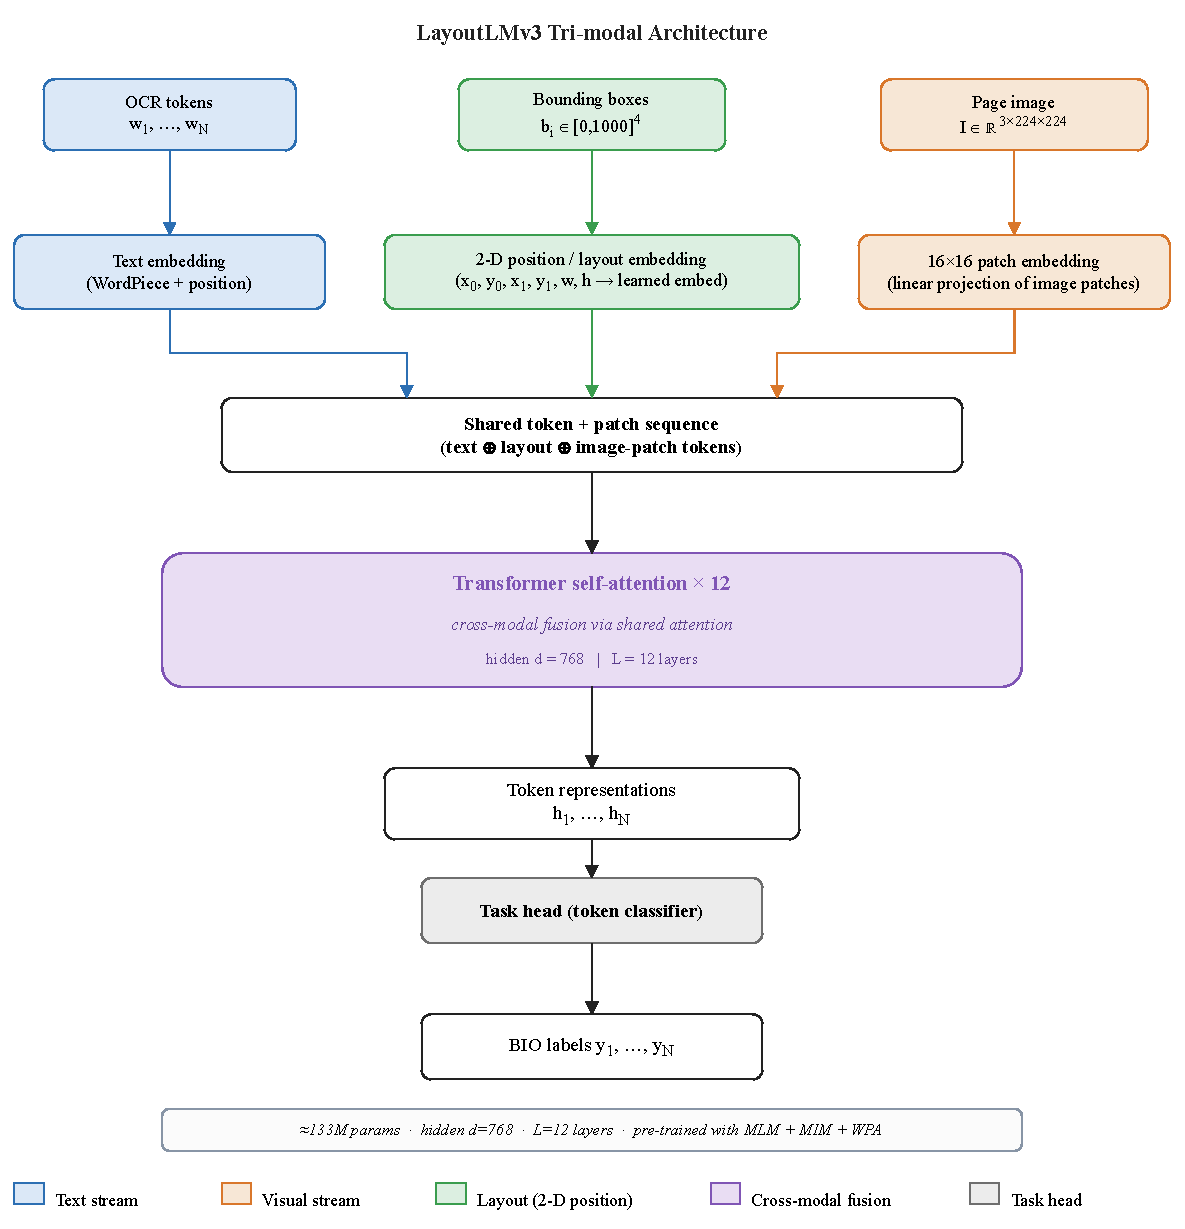
\includegraphics[width=0.72\linewidth]{layoutlmv3_components.pdf}
  \caption[The LayoutLMv3 encoder]{\textbf{The LayoutLMv3 encoder.} The \gls{ocr} tokens,
  their bounding boxes and the image patches are embedded into one sequence, which twelve
  transformer layers process jointly. A linear head maps the feature of every token to its
  \gls{bio} tag.}
  \label{fig:layoutlmv3-components}
\end{figure}

\paragraph{The fixed-label assumption.} All these models are trained once on all the data,
with a classifier sized to a fixed set of labels. However, real-world documents arrive in
sequence: a new vendor brings a new layout, a new language is added, and a new field must
be extracted that the earlier annotation did not cover. Retraining on all the data at each
change is costly, and it is not possible when the earlier documents may no longer be kept.
We use LayoutLMv3 as the main encoder of this thesis because it is the most widely adopted
encoder of this family, and LiLT, BROS and BERT to examine whether the findings depend on
the encoder (Chapter~\ref{ch:experimental-setup}).

% =============================================================================
\section{Catastrophic Forgetting and Continual Learning}
\label{sec:c2-s2}

\paragraph{Catastrophic forgetting.} Continual learning trains a model on a sequence of
sessions while it retains what it learned from the earlier ones. Its main obstacle is
catastrophic forgetting~\citep{mccloskey1989catastrophic}: when a network is trained on
new data only, the gradient steps overwrite the weights that encoded the old data, and the
old performance falls sharply. A model must therefore stay plastic enough to learn the new
session and stable enough to keep the old ones, which is known as the stability-plasticity
dilemma. Naive fine-tuning is fully plastic and forgets, whereas a frozen network is fully
stable and cannot learn. Every continual-learning method is a compromise between the two.

\paragraph{Scenarios.} The literature distinguishes three scenarios by what changes between
the sessions and what is known at test time~\citep{wang2024survey,masana2022class}. In
task-incremental learning, the identity of the session is given at test time, so a separate
classifier can be selected for it. In \gls{dil}, the label set is fixed and the input
distribution changes. In \gls{cil}, every session brings new classes, and the model must
separate all classes seen so far without knowing the session of a test sample. \Gls{cil}
is generally the hardest scenario, since the output space itself grows. In this thesis, we
study \gls{cil}, \gls{dil} and a mixed setting in which the classes and the domain change
together; their formal definition for \gls{kie} is given in
Section~\ref{sec:m-formulation}.

\paragraph{Method families.} Recent studies on catastrophic forgetting mainly consist of
regularisation, replay, optimisation-based methods, parameter isolation and methods built
on pre-trained models~\citep{wang2024survey}. Table~\ref{tab:cl-families} summarises them.

\emph{Regularisation} methods penalise the change of what the old sessions need. For
instance, \gls{ewc}~\citep{kirkpatrick2017ewc} adds to the loss of the new session a
quadratic penalty that is weighted by the Fisher information of the old ones,
\begin{equation}
  \mathcal{L}(\theta)=\mathcal{L}_{t}(\theta)+\frac{\lambda}{2}\sum_{i}F_{i}\,
  \big(\theta_{i}-\theta^{\ast}_{i}\big)^{2},
  \label{eq:ewc}
\end{equation}
where $\theta^{\ast}$ are the weights after the previous session and $F_i$ is the diagonal
of the Fisher information. SI~\citep{zenke2017si} and MAS~\citep{aljundi2018mas} estimate
the importance of a weight in other ways. As another example, \gls{lwf}~\citep{li2017lwf}
regularises the outputs instead of the weights: the model before the session serves as a
teacher, and the new model is distilled towards its predictions on the new data. These
methods store no sample, but they can only slow the change of the model down.

\emph{Replay} methods keep a small memory of past samples and train on them together with
the new data. \Gls{er}~\citep{rolnick2019er} stores raw samples with
their labels, and DER++~\citep{buzzega2020der} also stores the logits of the model at
storage time and distils towards them. iCaRL~\citep{rebuffi2017icarl} combines exemplars
with distillation and a nearest-mean classifier, and GEM~\citep{lopezpaz2017gem} and
A-GEM~\citep{chaudhry2019agem} use the memory as a constraint on the gradient. In a large
comparison of class-incremental methods, the best ones keep
exemplars~\citep{masana2022class}.

\emph{Optimisation-based} methods restrict the direction of the update. For instance,
OGD~\citep{farajtabar2020ogd} projects the gradient to be orthogonal to the gradients of
the old sessions, and GPM~\citep{saha2021gpm} projects it out of the subspace that the old
inputs span. \emph{Parameter-isolation} methods give every session its own parameters:
progressive networks~\citep{rusu2016pnn} add a column per session,
PackNet~\citep{mallya2018packnet} prunes and freezes a part of the weights after each
session, and DEN~\citep{yoon2018den} expands the network when needed. They do not forget by
construction; however, they need the identity of the session at test time, or a way to
infer it. Lastly, the methods built on a frozen pre-trained model are reviewed in
Section~\ref{sec:c2-s6}.

\begin{table}[!htbp]
  \centering
  \caption[Families of continual-learning methods]{\textbf{Families of continual-learning
  methods}: what each keeps across the sessions and its main limit for our setting.}
  \label{tab:cl-families}
  \small
  \begin{tabularx}{\textwidth}{@{}>{\raggedright\arraybackslash}p{2.4cm} >{\raggedright\arraybackslash}p{3.1cm} >{\raggedright\arraybackslash}p{3.0cm} >{\raggedright\arraybackslash}X@{}}
    \toprule
    Family & Examples & Kept across sessions & Limit for continual \gls{kie} \\
    \midrule
    Regularisation & \gls{ewc}, SI, MAS, \gls{lwf} & importance weights or the previous
      model & slows drift down, does not remove it \\
    Replay & \gls{er}, DER++, iCaRL, GEM & raw samples (and logits) & the stored labels
      become stale when the label set grows \\
    Optimisation & OGD, GPM & gradient or input subspaces & subspaces fill up over the
      sessions \\
    Parameter isolation & PNN, PackNet, DEN & parameters per session & needs the session
      identity at test time \\
    Pre-trained model & L2P, CODA-Prompt, LoRA variants, SLCA, RanPAC & prompts, adapters
      or class statistics & designed for image classification, with no background class \\
    \bottomrule
  \end{tabularx}
\end{table}

\paragraph{Measuring forgetting inside the network.} Besides the accuracy on old sessions,
forgetting can be measured inside the model. \citet{ramasesh2021anatomy} find that the
higher layers of a network change the most when it forgets, and that stabilising them
removes most of the forgetting. Two tools are commonly used for such an analysis. Linear
\gls{cka}~\citep{kornblith2019similarity} compares the
activations of one layer before and after a session on the same inputs; a value of one
means that the representation is unchanged up to a rotation and a scale. The Fisher
information~\citep{amari1998natural,kirkpatrick2017ewc} measures how much the loss of an
old session depends on each weight; weighting the displacement of a weight by it tells
whether the change matters. We use both tools in the analysis of drift
(Section~\ref{sec:m-drift}). For large multimodal models, forgetting after fine-tuning has
also been reported~\citep{zhai2023investigating}.

% =============================================================================
\section{The Background-Label Shift}
\label{sec:c2-s3}

When each session annotates only its own classes, one label changes its meaning from
session to session: the label that is given to everything else. In segmentation it is the
background class, in detection the unannotated regions, and in sequence labelling the tag
``O''. A region that is background in one session can be an object of a class that an
earlier or a later session annotates. This problem has been studied in three fields.

\paragraph{Semantic segmentation.} In class-incremental segmentation,
MiB~\citep{cermelli2020mib} first modelled the shift explicitly: in the cross-entropy, a
pixel labelled as background may be the background or any old class, so the probabilities
of the old classes are added to that of the background, and the distillation loss treats
the new classes in the mirrored way. PLOP~\citep{douillard2021plop} instead labels the
background pixels with the predictions of the old model and distils pooled features, and
SSUL~\citep{cha2021ssul} models an unknown class inside the background.
\citet{kalb2022causes} analyse the causes of forgetting in this setting and find that the
semantic shift of the background and the bias towards the new classes are the main ones;
\citet{kalb2023principles} extend the analysis to domain shift. For replay, a memory of
prototypes instead of images has been proposed to save storage~\citep{chen2023star}.

\paragraph{Object detection.} In incremental detection, the same problem appears on both
sides of a replay method. ABR~\citep{liu2023abr} observes that the stored images of old
sessions carry no boxes for the new classes, i.e., the stored side of the shift, and
replays stored boxes instead of whole images. BPF~\citep{mo2024bpf} addresses the past and
the future form together: an object of an old class and an object of a future class are
both unannotated in the current images.

\paragraph{Sequence labelling.} In continual \gls{ner}, it is known as the
unlabelled-entity problem~\citep{ma2023learning}: the entities of the other sessions appear
as ``O'' in the data of the current one. The methods mostly keep the model of the previous
session and use it on the tokens labelled ``O''. For instance,
ExtendNER~\citep{monaikul2021extendner} distils the predictions of the old model on these
tokens, and CFNER~\citep{zheng2022cfner} distils a causal effect that is computed from the
``O'' tokens. As another example, CPFD~\citep{zhang2023cpfd} combines a distillation of
pooled features with confidence-based pseudo-labels for the old entities, and
IS3~\citep{qiu2024is3} combines distillation with a debiased loss against the bias towards
the new classes. SpanKL~\citep{zhang2023spankl} avoids the token-level conflict by
classifying spans with one binary decision per class. Outside continual learning, the same
idea as in MiB appears for corpora with different tag sets: the likelihood is marginalised
over the tags that a corpus does not
annotate~\citep{greenberg2018marginal,beryozkin2019tagset}.

\paragraph{Limits for our setting.} These studies establish that the shift of the
background label exists and propose repairs on the side of the labels or of the loss.
However, three questions remain open for a replay method on documents. First, most repairs
assume no memory, and it is unclear how the shift interacts with a memory whose stored
labels were written under an older label set. Second, the repairs are compared by their
final accuracy; it has not been measured which part of the gap a correct label would close
and which part remains. Third, the methods for sequence labelling are validated on text,
where a sentence holds few entities, whereas a document page holds many entities of several
sessions. We do not claim the conflict itself; instead, we separate what a memory repairs
from what survives correct stored labels (Section~\ref{sec:m-hypotheses}).

% =============================================================================
\section{Separated Readouts and Session Identification}
\label{sec:c2-s4}

A second line of work changes the output layer instead of the labels.

\paragraph{Separating the softmax.} A softmax over old and new classes together biases the
scores towards the new classes, since the old ones are seen rarely.
SS-IL~\citep{ahn2021ssil} separates the softmax of the old classes from that of the new
ones and adds a task-wise distillation, which reduces the bias. As another example,
ER-ACE~\citep{caccia2022erace} restricts the softmax of the incoming samples to their own
classes, while the replayed samples use all classes. These methods are designed for image
classification, where every sample has exactly one class and no class plays the role of a
background.

\paragraph{Session identification.} \citet{kim2022theoretical} show that class-incremental
learning decomposes into two problems: predicting the class within a session, and
identifying the session, which is equivalent to detecting out-of-distribution samples for
each session. Based on this result, MORE~\citep{kim2022more} isolates the parameters of
each session on a pre-trained model and trains an out-of-distribution output per head from
saved samples. On text information extraction, ICE~\citep{liu2023ice} freezes the encoder
and trains one classifier per session; its variant ICE-O gives every session a softmax
over its classes and a constant logit for the class ``Other'', and predicts the class with
the largest logit over all sessions. A background output per session is thus a known
component.

\paragraph{Limits for our setting.} Unlike them, we study this readout on token-labelled
documents together with a memory. ICE keeps the encoder frozen and uses no memory; hence,
it cannot adapt the representation to a new session, and its background logit is a
constant. MORE needs saved raw samples and one set of isolated parameters per session. It
is unclear which of the components (a memory, a separated normalisation, a learned
background) is necessary, and whether a separated readout alone is sufficient when the
encoder keeps training. Our study answers these questions with one component removed at a
time (Section~\ref{sec:c6-s4}).

% =============================================================================
\section{Latent and Compressed Replay}
\label{sec:c2-s5}

Raw replay stores the samples themselves, which is costly and, for documents, means keeping
the page images and the text of past customers. Several lines of work reduce what is
stored.

\paragraph{Latent replay.} Instead of the input, latent replay stores the activations of an
intermediate layer and replays them into the layers above it. REMIND~\citep{hayes2020remind}
freezes the layers below, quantises the stored activations and can therefore keep many more
samples in the same memory. \citet{pellegrini2020latent} slow the lower layers down instead
of freezing them, for learning on devices. Generative variants replay internal
representations that a learned generator produces~\citep{vandeven2020brain}.

\paragraph{Replay without samples.} Other methods keep only statistics of the features. For
instance, PASS~\citep{zhu2021pass} keeps one prototype per class and augments it, as another
example FeTrIL~\citep{petit2023fetril} translates the features of new classes to the
prototypes of old ones, and FeCAM~\citep{goswami2023fecam} keeps the class covariances for
a distance-based classifier. On a pre-trained model, SLCA~\citep{zhang2023slca} and
RanPAC~\citep{mcdonnell2023ranpac} follow the same idea (Section~\ref{sec:c2-s6}). These
methods are designed for image classification, where one feature vector summarises one
sample.

\paragraph{Limits for our setting.} For token labelling, a sample is a whole document: the
label of a token depends on the other tokens of the page through self-attention. It is
unclear whether per-class statistics of token features can replace the document, and a
memory of activations must keep all positions of a page, which is large. Besides, whereas
most prior replay mechanisms focus on which samples to store or how to compress them, they
do not ask what the stored labels say. Under label growth, a stored document carries the
background label on every entity outside its session, whatever the format of the memory. We
therefore use a latent memory that keeps the whole document in compressed form
(Section~\ref{sec:m-colar}) and study the stored labels separately.

% =============================================================================
\section{Continual Learning with Pre-trained Models}
\label{sec:c2-s6}

More recently, methods built on a frozen pre-trained model have become the dominant
approach in class-incremental image classification. They consist of three groups.

\paragraph{Prompts.} L2P~\citep{wang2022l2p} keeps the model frozen and learns a pool of
prompts, from which a query selects the prompts of a test sample.
DualPrompt~\citep{wang2022dualprompt} splits the prompts into general and
session-specific ones, and CODA-Prompt~\citep{smith2023coda} replaces the selection with a
weighted combination that is trained end to end.

\paragraph{Low-rank adapters.} LoRA~\citep{hu2022lora} adapts a frozen weight matrix with
the product of two small matrices. For continual learning, O-LoRA~\citep{wang2023olora}
keeps the adapters of different sessions in orthogonal subspaces,
InfLoRA~\citep{liang2024inflora} designs the subspace so that a new adapter does not
interfere with the old sessions, CL-LoRA~\citep{he2025cllora} combines adapters shared by
all sessions with session-specific ones, and SD-LoRA~\citep{wu2025sdlora} separates the
magnitude and the direction of the updates.

\paragraph{Classifier alignment.} A third group observes that, on a strong pre-trained
model, most of the forgetting sits in the classifier. SLCA~\citep{zhang2023slca} trains the
encoder with a small learning rate and re-aligns the classifier with features sampled from
class-wise Gaussian statistics. RanPAC~\citep{mcdonnell2023ranpac} projects the frozen
features randomly to a higher dimension and builds the classifier from class prototypes,
and EASE~\citep{zhou2024ease} trains one adapter per session and completes the prototypes
of the old classes in each new subspace. Recently, LCA~\citep{lca2026} merges the models of
the sessions and aligns the classifier afterwards.

\paragraph{Limits for our setting.} These methods are mainly designed for image
classification and validated there. It is a non-trivial task to apply them to token
labelling, for two reasons. First, there is no class in image classification that plays the
role of the background; a classifier that is rebuilt from the statistics of each class has
no rule for a label whose meaning changes with the session. Second, the frozen model
suffices when the pre-trained features already separate the classes, whereas a new document
domain or a new schema needs the encoder to adapt. Besides, it has been shown that the
ranking of continual-learning methods depends strongly on how their hyper-parameters are
chosen~\citep{cha2025hyperparameters}, which calls for one protocol for all methods. We
include CODA-Prompt, CL-LoRA and LCA as baselines under one protocol
(Section~\ref{sec:e-baselines}).

% =============================================================================
\section{Continual Learning for Document Understanding}
\label{sec:c2-s7}

There have been few works on continual learning for documents.

\paragraph{Continual information extraction on text.} Most of the work on continual
information extraction is on sentences. Besides the continual \gls{ner} methods of
Section~\ref{sec:c2-s3}, continual relation extraction keeps a small memory of exemplars
and prototypes of the relations~\citep{han2020emar,cui2021rpcre,zhao2022crl}. These methods
use no layout and no image, and their benchmarks contain a few entities per sentence.

\paragraph{Documents.} For documents, continual table detection uses plain
\gls{er}~\citep{minouei2022table}, and ProtoNER~\citep{kumar2023protoner} adds new entity
classes to a layout-aware model with prototypes from a few examples. GDI-Bench~\citep{gdibench}
evaluates multimodal language models on document tasks of graded difficulty and studies
their fine-tuning. Recently, \citet{sassioui2026documents} benchmarked the forgetting of
layout-aware models under domain, layout and schema shifts, and a gradient-projection
method was proposed for the same setting~\citep{sassioui2026amdproj}. However, they
decompose forgetting by the kind of shift, whereas we decompose it by its cause.

\paragraph{Multimodal models.} Continual learning has also been studied for
vision-and-language tasks such as visual question
answering~\citep{srinivasan2022climb,zhang2025clcrossvqa,lei2023clove}. These benchmarks
contain no token-level extraction and no background label.

% =============================================================================
\section{Research Gaps and Positioning}
\label{sec:c2-s8}

From the review above, we identify three gaps.

\paragraph{Gap 1: the cause of forgetting in continual \gls{kie} is not separated.} Prior
work on documents reports how much a model forgets under each kind of shift. Prior work on
the background shift shows that the labels change their meaning. However, there exists no
study that separates, on the same model and the same streams, the forgetting that comes
from the drift of the representation from the failure that comes from the background
label. Without this separation, it is unclear what a remedy must repair.

\paragraph{Gap 2: replay under label growth is not understood.} Replay is the strongest
family in class-incremental image classification. For token labelling, a replay memory
carries background labels that were written under an older label set, and the current
documents carry background labels on the entities of the old sessions. Furthermore, it is
unclear which of the two sides matters, and whether correcting the labels would be enough.

\paragraph{Gap 3: no method combines a memory against drift with a readout against the
conflict.} The methods with a separated readout either freeze the encoder or isolate its
parameters, and the methods with a memory keep one softmax over all classes. To our
knowledge, on token-labelled documents, no prior work combines a memory against drift with
one learned background per session, and none measures what each one repairs.

\paragraph{Positioning.} Table~\ref{tab:positioning} compares our work with the closest
studies. We address Gap~1 with an analysis protocol that measures the drift by depth and
tests three hypotheses on the background conflict (Sections~\ref{sec:m-drift}
and~\ref{sec:m-hypotheses}). We address Gap~2 with interventions that repair the stored
side and the current side of the labels one at a time (Section~\ref{sec:c6-s2}). We address
Gap~3 with CoLaR-SBR, which takes a compressed latent memory against the drift and a
session-blocked readout against the conflict, and with SBR-Recall, its variant without
stored documents (Sections~\ref{sec:m-colar} to~\ref{sec:m-recall}).

\begin{table}[!htbp]
  \centering
  \caption[Positioning against the closest studies]{\textbf{Positioning against the closest
  studies.} Memory: what is kept from the old sessions. Background: how the shift of the
  background label is treated (``n/a'': the task has no background class). Per session:
  the output is normalised within each session. Encoder: whether the encoder is trained in
  every session.}
  \label{tab:positioning}
  \footnotesize\setlength{\tabcolsep}{4pt}
  \begin{tabularx}{\textwidth}{@{}>{\raggedright\arraybackslash}p{2.7cm} >{\raggedright\arraybackslash}p{1.8cm} >{\raggedright\arraybackslash}p{2.1cm} >{\raggedright\arraybackslash}X >{\raggedright\arraybackslash}p{1.7cm} >{\raggedright\arraybackslash}p{1.7cm}@{}}
    \toprule
    Study & Task & Memory & Background & Per session & Encoder \\
    \midrule
    \gls{er}, DER++ & images & raw samples & n/a & no & trained \\
    REMIND, latent replay & images & activations & n/a & no & upper layers \\
    SS-IL & images & raw samples & n/a & old against new & trained \\
    ER-ACE & images & raw samples & n/a & incoming samples & trained \\
    MORE & images & raw samples & n/a & yes & isolated \\
    MiB, PLOP & segmentation & previous model & marginal loss, pseudo-labels & no &
      trained \\
    CPFD, IS3 & text \gls{ner} & previous model & pseudo-labels, debiased distillation &
      no & trained \\
    ICE-O & text extraction & none & constant logit per session & yes & frozen \\
    \citet{sassioui2026documents} & documents & benchmark of baselines & not treated & no
      & trained \\
    \midrule
    CoLaR-SBR (ours) & documents & compressed activations & learned logit per session &
      yes & upper layers \\
    SBR-Recall (ours) & documents & low-rank updates & learned logit per session & yes &
      frozen after session 1 \\
    \bottomrule
  \end{tabularx}
\end{table}

% =============================================================================
\section{Chapter Summary}
\label{sec:c2-s9}

In this chapter, we reviewed layout-aware document models, the families of
continual-learning methods and the four lines of work closest to ours. The shift of the
background label is known in segmentation, detection and continual \gls{ner}, and a
background output per session is known from text information extraction. However, the
causes of forgetting in continual \gls{kie} have not been separated, replay under label
growth is not understood, and no method combines a memory against drift with a readout
against the conflict. The next chapter presents our analysis protocol and our method.

% Chapter 3 (two-cause rewrite, 2026-11). No result number in this chapter: results are in Ch. 6.
% Old text: chapters_old/chapter3.tex (git tag thesis-pre-two-causes).
\chapter{Methodology}
\label{ch:methodology}

This chapter presents how we study forgetting in continual \gls{kie} and how we address it.
In the following, we first formalise the problem and the metrics
(Section~\ref{sec:m-formulation}). Then, we describe how we analyse the two causes of
forgetting that this thesis separates: the drift of the representation
(Section~\ref{sec:m-drift}) and the conflict on the background label
(Section~\ref{sec:m-conflict}). After that, we detail the proposed method, CoLaR-SBR, and its
variant SBR-Recall (Sections~\ref{sec:m-overview} to~\ref{sec:m-recall}). Finally, we account
for its memory and compute cost (Section~\ref{sec:m-accounting}). All results are reported in
Chapter~\ref{ch:results}.

% =============================================================================
\section{Problem Formulation and Metrics}
\label{sec:m-formulation}

\paragraph{Continual key-information extraction.} A document is defined as
$x=(w_{1:L},\,b_{1:L},\,I)$, where $w_{1:L}$ are its \gls{ocr} tokens, $b_{1:L}$ their
normalised bounding boxes and $I$ the page image. A model $f_\theta$ labels every token with
a \gls{bio} tag, and the entities are scored by entity-level F1~\citep{tjong2003conll}. The
model consists of an encoder, which maps the document to one feature vector $h(x_i)\in
\mathbb{R}^{d}$ per token, and a linear head, which maps the feature to the tag logits
$z(x_i)$.

The documents arrive in $T$ sessions. Session $t$ brings a training set $\mathcal{D}_t$ that
is annotated with its own tag set $\mathcal{T}_t$ only. Specifically, a token whose true tag
is $y^{\ast}$ is labelled
\begin{equation}
  y=\begin{cases} y^{\ast} & y^{\ast}\in\mathcal{T}_t,\\ \mathrm{O} & \text{otherwise.}\end{cases}
  \label{eq:mask}
\end{equation}
In the \gls{bio} scheme, ``O'' is the tag of every token that belongs to no annotated entity.
From now on, we call it the \emph{background label}: we write ``O'' when we refer to the tag in
the data, and background label when we refer to its role in training. Under
Equation~\eqref{eq:mask}, the background label of session $t$ covers two kinds of tokens: the
tokens that are truly not entities, and the entities that session $t$ does not annotate. While
the model learns session $t$, it has no access to the training sets of the earlier sessions,
except for what a bounded memory keeps. After the last session, the model is tested on the
classes of all sessions, without knowing which session a document comes from.

\paragraph{Three settings.} We study three settings, which differ in what changes between
two sessions. In \gls{cil}, the tag set grows and the documents stay in one domain. This is
the setting where the background label changes its meaning from one session to the next;
hence, it is where our main claims are tested. In \gls{dil}, the tag set is fixed and the
documents change, e.g., from forms to receipts. Since every session annotates all classes,
Equation~\eqref{eq:mask} masks nothing; thus, forgetting can only come from the change of the
model itself, and \gls{dil} serves as the control without the conflict. In the \emph{Mixed}
setting, both change, which tests the two causes together. The six streams that instantiate
these settings on five public datasets are described in Chapter~\ref{ch:experimental-setup}.

\paragraph{Retention matrix.} To measure what the model keeps, we hold one test split per
session, masked like its training set. Let $R[i,j]$ be the F1 on the test split of session
$j$ after the model has been trained on session $i$. From this matrix, we report the
\gls{aa} and the \gls{af}:
\begin{equation}
  \mathrm{AA}=\frac{1}{T}\sum_{j=1}^{T}R[T,j],\qquad
  \mathrm{AF}=\frac{1}{T-1}\sum_{j=1}^{T-1}\big(R[j,j]-R[T,j]\big).
  \label{eq:aa-af}
\end{equation}
\gls{aa} is the mean F1 of the final model over the sessions. \gls{af} is the F1 of a session
right after it was learned minus its final F1, averaged over the sessions before the last
one. It is noted that the diagonal $R[j,j]$ matters on its own: it tells whether a session
was learned at all, which a single final number cannot show.

\paragraph{Session-restricted scoring.} The test labels of session $j$ show only its own
classes. Hence, raw scoring would charge a model for every correct entity of another
session: such an entity is labelled ``O'' in the split of session $j$, so predicting it
counts as a false positive. To avoid this, we score each split \emph{session-restricted}: a
predicted tag outside $\mathcal{T}_j$ is mapped to ``O'' before the spans are matched. As a
result, a predicted entity can be a false positive only in its own session, and a missed
entity is counted only in its own session.

\paragraph{Full-label F1.} Session-restricted scoring has two limits. The test split of a
session keeps only the documents that contain one of its entities, and \gls{aa} weights all
sessions equally, although they hold different numbers of entities. Hence, on the
class-incremental streams we also report the \emph{full-label F1}: the entity-level F1 of
the final model on the complete test set with all classes and no label masked, as in
continual named entity recognition~\citep{ma2023learning}. The full-label F1 is our headline
number on the class-incremental streams, and \gls{aa} and \gls{af} describe retention on
every stream. Table~\ref{tab:notation} summarises the notation of this chapter.

\begin{table}[!htbp]
  \centering
  \caption[Notation of the methodology]{\textbf{Notation.} Symbols used in this chapter.}
  \label{tab:notation}
  \begin{tabular}{@{}ll@{}}
    \toprule
    Symbol & Meaning \\
    \midrule
    $T$, $t$ & number of sessions; index of the current session \\
    $\mathcal{D}_t$, $\mathcal{T}_t$ & training set and tag set of session $t$ \\
    $h(x)\in\mathbb{R}^{d}$, $z(x)$ & feature and tag logits of a token $x$ \\
    $R[i,j]$ & F1 on the test split of session $j$ after training session $i$ \\
    $k$, $r$ & layer where the memory is injected; rank of its compression \\
    $H_j\in\mathbb{R}^{L\times d}$ & layer-$k$ activations of the stored document $j$ \\
    $b$, $\mathcal{T}_b$ & a readout block and the tags it holds \\
    $o_b(x)$, $p_b(\cdot\mid x)$ & background logit and distribution of block $b$ \\
    $m_{sb}$ & whether a document of session $s$ supervises block $b$ \\
    $e_b(x)$ & claim of block $b$ on a token, $1-p_b(\mathrm{O}_b\mid x)$ \\
    $\theta_0$, $\Delta_b$ & frozen encoder state and the low-rank update of block $b$ \\
    \bottomrule
  \end{tabular}
\end{table}

% =============================================================================
\section{Analysing Cause 1: Representation Drift}
\label{sec:m-drift}

The first cause of forgetting is the drift of the model. When the encoder is trained on a
new session, the features that it computes for the documents of the old sessions change, and
the head that was fitted on the old features no longer reads them correctly. This cause does
not depend on the labels; it is present even when the label space is fixed. In this section,
we describe how we measure the drift and how we test what removes it.

\paragraph{Representational drift.} To measure how much the representation of a layer
changes, we use linear \gls{cka}~\citep{kornblith2019similarity}. Given two centred
activation matrices $X\in\mathbb{R}^{n\times p}$ and $Y\in\mathbb{R}^{n\times q}$ of the same
$n$ inputs,
\begin{equation}
  \mathrm{CKA}(X,Y)=\frac{\lVert Y^{\top}X\rVert_F^{2}}
  {\lVert X^{\top}X\rVert_F\,\lVert Y^{\top}Y\rVert_F}.
  \label{eq:cka}
\end{equation}
We compute it between the activations of the model before and after a session on a fixed
probe set; a value of $1$ means that the layer did not drift. Two choices matter here.
First, token classification reads one feature per token; hence, we compute \gls{cka} over
individual tokens and not over the mean vector of a document, which could report no drift
while the features of the tokens have been reorganised. Second, the probe set holds more
tokens than the width of the layer, so that the estimate is stable.

\paragraph{Importance and displacement.} \gls{cka} tells where the features change. To tell
where the \emph{parameters} that mattered for an old session are overwritten, we use two
quantities per parameter group $g$. The empirical Fisher importance on the data
$\mathcal{D}$ of a session,
\begin{equation}
  F_g=\frac{1}{|\mathcal{D}|}\sum_{(x,y)\in\mathcal{D}}\;\sum_{\phi\in g}
  \Big(\frac{\partial\log p_\theta(y\mid x)}{\partial\phi}\Big)^{2},
  \label{eq:fisher}
\end{equation}
measures how sensitive the loss of that session is to the group. It is noted that importance
alone is not a sign of forgetting: the head carries the largest gradients of any token
classifier, whether or not its parameters are moved later. Hence, we weight the change of the
parameters between two checkpoints by the importance of the old session,
\begin{equation}
  D_g=\sum_{\phi\in g}F^{(t-1)}_{\phi}\,\big(\theta^{(t)}_{\phi}-\theta^{(t-1)}_{\phi}\big)^{2},
  \label{eq:displacement}
\end{equation}
which is large exactly where parameters that mattered before session $t$ have been changed
by session $t$. We report the three quantities by depth, in five groups: the input
embeddings, the early, middle and late layers, and the head.

\paragraph{Protocol.} We fine-tune the model naively on a stream, i.e., one session after the
other with no continual-learning method, and keep a checkpoint at every session boundary.
At each boundary, we compute \gls{cka}, the Fisher importance and the displacement between
the two checkpoints, together with one row of the retention matrix
(Algorithm~\ref{alg:drift}). To examine whether the picture depends on the encoder, we repeat
the analysis on four encoders: LayoutLMv3~\citep{huang2022layoutlmv3}, which reads text,
layout and the page image; LiLT~\citep{wang2022lilt} and BROS~\citep{hong2022bros}, which
read text and layout; and BERT~\citep{devlin2019bert}, which reads text only. On LayoutLMv3,
we additionally repeat it with some of the inputs masked (text only, text and layout, image
and layout), so that the architecture is fixed and only the inputs differ.

\begin{algorithm}[!htbp]
  \caption{Drift analysis at the session boundaries}
  \label{alg:drift}
  \begin{algorithmic}[1]
    \Require sessions $\mathcal{D}_{1:T}$, probe set $\mathcal{P}$, layers $\mathcal{G}$, parameter groups $\mathcal{G}_F$
    \State initialise $\theta^{(0)}$ from the pre-trained encoder
    \For{$t=1$ \textbf{to} $T$}
      \State grow the head by the tags $\mathcal{T}_t$
      \State $\theta^{(t)}\gets\textsc{FineTune}(\theta^{(t-1)},\mathcal{D}_t)$ \Comment{naive, no memory}
      \ForAll{$\ell\in\mathcal{G}$}
        \State $\mathrm{CKA}_{t,\ell}\gets\textsc{LinearCKA}\big(\textsc{Act}_\ell(\theta^{(t-1)},\mathcal{P}),\,\textsc{Act}_\ell(\theta^{(t)},\mathcal{P})\big)$
      \EndFor
      \ForAll{$g\in\mathcal{G}_F$}
        \State $F_{t,g}\gets\textsc{Fisher}(\theta^{(t)},g,\mathcal{D}_t)$;\quad
               $D_{t,g}\gets\sum_{\phi\in g}F^{(t-1)}_{\phi}(\theta^{(t)}_{\phi}-\theta^{(t-1)}_{\phi})^{2}$
      \EndFor
      \State $R[t,j]\gets\textsc{F1}(\theta^{(t)},\text{test split of session } j)$ for all $j\le t$
    \EndFor
    \State \Return $\mathrm{CKA}$, $F$, $D$, $R$
  \end{algorithmic}
\end{algorithm}

\paragraph{What removes the drift.} The measurement tells where the drift sits, not what
removes it. To examine the latter, we compare the main families of continual learning on the
domain-incremental stream, where drift is the only cause: regularisation of the
parameters~\citep{kirkpatrick2017ewc}, distillation from the previous
model~\citep{li2017lwf} and replay of old documents~\citep{rolnick2019er,buzzega2020der},
against naive fine-tuning and joint training. If drift is what a method must counter, then a
method that shows old documents to the model again should come close to joint training on
this stream, whereas a method that only constrains the parameters may not. This comparison is
repeated on the four encoders (Section~\ref{sec:c6-s1}), and its outcome decides the starting
point of our method.

% =============================================================================
\section{Analysing Cause 2: The Background-Label Conflict}
\label{sec:m-conflict}

The second cause appears only when the tag set grows. In this section, we first show where
the conflict comes from, and then state the series of hypotheses with which we test it.

\subsection{Where the Conflict Comes From}
\label{sec:m-conflict-origin}

Consider the usual readout, one softmax over the background label and all classes seen so
far,
\begin{equation}
  p(c\mid x)=\frac{\exp z_c(x)}{\exp z_{\mathrm{O}}(x)+\sum_{c'\in\mathcal{T}_{1:t}}\exp z_{c'}(x)},
  \qquad c\in\{\mathrm{O}\}\cup\mathcal{T}_{1:t},
  \label{eq:shared}
\end{equation}
where $\mathcal{T}_{1:t}=\bigcup_{s\le t}\mathcal{T}_s$. We refer to it as the \emph{shared
softmax}. For a token that is labelled ``O'', the gradient of the cross-entropy with respect
to the logits is
\begin{equation}
  \frac{\partial\mathcal{L}}{\partial z_{\mathrm{O}}}=p(\mathrm{O}\mid x)-1\le 0,\qquad
  \frac{\partial\mathcal{L}}{\partial z_c}=p(c\mid x)\ge 0\quad\text{for every } c\in\mathcal{T}_{1:t}.
  \label{eq:grad}
\end{equation}
Thus, one background token raises the background logit and lowers the logit of \emph{every}
class in the head, including the classes that its session did not annotate. Under
Equation~\eqref{eq:mask}, this happens on two sides (Figure~\ref{fig:conflict}).

\begin{itemize}
  \item \textbf{Current side.} A document of the current session $t$ labels every entity of
        an earlier session as ``O''. Hence, each training step lowers the logits of the old
        classes on tokens that truly belong to them.
  \item \textbf{Stored side.} A document that was stored at session $s<t$ labels every entity
        of a later session as ``O''. Hence, each replay step lowers the logits of the new
        classes on tokens that truly belong to them. The stored labels are \emph{stale}: they
        were complete when the document was stored and became wrong when the head grew.
\end{itemize}

\noindent As a result, the same token receives contradicting labels over time, and the
single background logit $z_{\mathrm{O}}$ is trained by documents that disagree on what the
background is. It is noted that a memory does not remove this conflict. On the contrary,
replay adds the stored side to it; this is why we treat the conflict as a cause of its own
and not as a harder form of drift. The shift of the background label is known from continual
semantic segmentation~\citep{cermelli2020mib} and continual named entity
recognition~\citep{zhang2023cpfd,ma2023learning}, and its two sides were named in continual
object detection~\citep{liu2023abr,mo2024bpf}. However, it is unclear which side matters in
document streams, and whether repairing the labels is enough.

\subsection{A Series of Hypotheses}
\label{sec:m-hypotheses}

We examine the failure of replay under label growth with three hypotheses. Each one makes a
prediction, and each is tested by changing one intervention against the run it is compared
with (Table~\ref{tab:hypotheses}). For each hypothesis, we report whether its prediction
holds, fails or holds in part.

\paragraph{H1: only harder forgetting.} We first hypothesize that label growth only makes
forgetting harder, i.e., that the failure is still caused by drift. If so, a memory that
works under domain shift should also work under label growth, and a larger memory should
close the remaining gap. To examine it, we take the same memory with the shared softmax from
the domain-incremental stream to the class-incremental one, we vary its size, and we replace
the stored activations by raw documents. We also read the diagonal of the retention matrix:
under drift alone, a session is learned well and lost later, whereas under the conflict the
session that is being trained may not be learned in the first place.

\paragraph{H2: the labels are the cause.} We next hypothesize that the labels are the cause,
on the two sides above. If so, repairing the labels should close the gap with the shared
softmax unchanged. On the stored side, we repair the labels with the ground-truth labels,
which a continual learner does not have, in two ways: every stored document receives the
true labels of all classes in the grown head before each session; or the stale tokens are
masked in the replay loss, which removes the false background label without adding a label.
On the current side, we use two repairs that need no additional annotation. The first one
follows the unbiased cross-entropy of MiB~\citep{cermelli2020mib}: a background token is
allowed to be the background \emph{or} any class that its document could not annotate,
\begin{equation}
  \mathcal{L}_{\mathrm{MiB}}(x,\mathrm{O},s)=-\log\Big(p(\mathrm{O}\mid x)
  +\sum_{c\,\in\,\mathcal{T}_{1:t}\setminus\mathcal{T}_s}p(c\mid x)\Big),
  \label{eq:mib}
\end{equation}
where $s$ is the session of the document, so that the sum runs over the earlier classes for
a current document and over the later classes for a stored one. The second one slices the
softmax: the loss of a stored document is normalised over the classes that were known when it
was stored, and, in a further control inspired by SS-IL~\citep{ahn2021ssil}, the loss of the
current background tokens is normalised without the old classes.

\paragraph{H3: the shared normalisation.} Finally, we hypothesize that the conflict lives in
the shared normalisation itself: one background logit that is trained by documents which
disagree on the background. If so, giving each session its own background logit, normalised
with the tags of that session only, should close most of the gap without any additional
annotation. This is the diagnosis of SS-IL for a shared softmax~\citep{ahn2021ssil} with a
background label added, and the readout of ICE-O~\citep{liu2023ice} without its frozen
encoder. We test it with and without the memory, in order to separate what the readout
contributes from what replay contributes.

\begin{table}[!htbp]
  \centering
  \caption[The series of hypotheses and their tests]{\textbf{The series of hypotheses.}
  Each hypothesis is tested by one change against the memory with a shared softmax.
  $^{r}$Uses the ground-truth labels of the stored documents.}
  \label{tab:hypotheses}
  \begin{tabularx}{\textwidth}{@{}l>{\raggedright\arraybackslash}p{4.3cm}L@{}}
    \toprule
    Hypothesis & Intervention & Prediction if the hypothesis holds \\
    \midrule
    H1 only harder forgetting & same memory as on \gls{dil}; larger memory; raw documents &
      the gap to joint training closes as on \gls{dil}; every session is learned when it is trained \\
    \addlinespace
    H2 the labels (stored side) & true labels before each session$^{r}$; stale tokens masked$^{r}$ &
      the shared softmax reaches joint training on every stream \\
    H2 the labels (current side) & MiB-style loss (Equation~\ref{eq:mib}); softmax slices &
      the gap closes without ground-truth labels \\
    \addlinespace
    H3 the shared normalisation & one background logit per session, with and without the memory &
      most of the gap closes on every stream, with no additional annotation \\
    \bottomrule
  \end{tabularx}
\end{table}

\noindent The three hypotheses are tested on the three class-incremental streams in
Section~\ref{sec:c6-s2}. The outcome of H3 motivates the readout of our method.

% =============================================================================
\section{Overview of the Proposed Method}
\label{sec:m-overview}

In this work, we aim to remove the two causes: the drift of the encoder and the conflict on
the background label. The workflow of the proposed method, CoLaR-SBR, is shown in
Figure~\ref{fig:method}. Given the documents of a session, the model is trained on them as
usual. After the session, we store a few of its documents as compressed activations of an
intermediate layer (step~1). Then, while the model learns a new session, we replay the
stored documents to remind the model of the past sessions (step~2); this addresses the
drift. Finally, every session reads its tokens with its own background logit (step~3), so
that the background label of one session is never counted against the classes of another;
this addresses the conflict. A variant, SBR-Recall, keeps one low-rank update of the encoder
per session in place of the memory.

\begin{figure}[!htbp]
  \centering
  \papertikz{0.95}{figures/paper/tikz_method}
  \caption[Overview of CoLaR-SBR]{\textbf{Overview of CoLaR-SBR.} Documents are (1) stored
  and (2) replayed as layer-$k$ activations; (3) each session reads its tokens with its own
  background logit (b), not with a shared one (a). SBR-Recall keeps one low-rank update per
  session and no memory.}
  \label{fig:method}
\end{figure}

\paragraph{The principle.} We argue that a token labelled as background in session $s$ means
``none of the classes annotated in session $s$''. It is evidence against those classes and
silent about every other class, as in training on partially annotated
data~\citep{greenberg2018marginal}. Hence, we \emph{supervise each class only with negatives
from documents that annotated it, and normalise together only the classes that were annotated
together}. The repairs of H2 follow the same principle on the side of the labels or of the
loss; our readout follows it in the normalisation, where no label needs to be repaired.

% =============================================================================
\section{CoLaR: Compressed Latent Replay}
\label{sec:m-colar}

The readout of Section~\ref{sec:m-sbr} needs stored documents that keep the label of each
token at its position, together with the session that wrote the labels. Hence, our memory
keeps \emph{whole documents}, not statistics of classes. Inspired by latent
replay~\citep{hayes2020remind,pellegrini2020latent}, CoLaR (Compressed Latent Replay) stores a
document as the activations of an intermediate layer and not as its raw page. It works in
three steps.

\paragraph{Freezing the lower layers.} First, after the first session, we freeze the input
embeddings and the layers $1..k$ of the encoder. A stored activation stays valid only while
the layers below it do not change; with these layers frozen, an activation that was stored at
any session is exactly what the current model would compute for the same document.

\paragraph{Storing.} Then, at the end of each session, we draw $N$ documents at random from
its training set. For each document $j$, we take its layer-$k$ activations
$H_j\in\mathbb{R}^{L\times d}$, where $L$ is the number of positions of the document, and
compress them with a truncated \gls{svd} of rank $r$,
\begin{equation}
  H_j\approx U_j\Sigma_jV_j^{\top},\qquad U_j\in\mathbb{R}^{L\times r},\;
  \Sigma_j\in\mathbb{R}^{r\times r},\;V_j\in\mathbb{R}^{d\times r}.
  \label{eq:svd}
\end{equation}
We store the factors $U_j\Sigma_j$ and $V_j$ in half precision, with the boxes, the attention
mask, the labels and the session of the document. It is noted that the compression is
applied to one document at a time. The features of all documents together are close to full
rank, whereas the activations of a single document are not, since its tokens share one
layout and one vocabulary; thus, a per-document factorisation keeps the document faithfully
at a rank far below $d$. No pixel and no token id is kept.

\paragraph{Replaying.} Finally, at every training step, we draw stored documents, rebuild
their activations $H_j$ from the factors and inject them at layer $k{+}1$, where the boxes
and the mask of the document drive the layout biases and the attention mask as for a current
document. The upper layers and the head are then trained on the current batch and on the
replayed documents together. We use $k{=}4$, $r{=}128$ and $N{=}50$ documents per session;
the impact of each setting is studied in Section~\ref{sec:c6-s5}.

\paragraph{Why activations and not raw documents.} A memory of raw documents would serve the
readout as well, and we compare both in Section~\ref{sec:c6-s4}. We choose the latent memory
for two reasons. First, it holds neither pixels nor token ids. Second, a replayed document
passes only through the layers above $k$; hence, replay trains fewer parameters than raw
replay does. We do not claim that it is smaller than a raw document in every encoding
(Section~\ref{sec:m-accounting}).

% =============================================================================
\section{SBR: Session-Blocked Readout}
\label{sec:m-sbr}

SBR (Session-Blocked Readout) is our instantiation of a readout with one background per
session~\citep{liu2023ice,kim2022more}. In the following, we describe its blocks, its
training rule and its inference rule.

\paragraph{Blocks.} Every session that brings new tags opens a \emph{block} $b$ that holds
those tags $\mathcal{T}_b$. Whereas the shared softmax of Equation~\eqref{eq:shared}
normalises over the background label and all classes, SBR gives every block its own
background logit, a linear map of the token feature,
\begin{equation}
  o_b(x)=w_b^{\top}h(x)+c_b,
  \label{eq:olog}
\end{equation}
and normalises each block separately:
\begin{equation}
  p_b(\cdot\mid x)=\operatorname{softmax}\big([\,o_b(x),\,z_{\mathcal{T}_b}(x)\,]\big),
  \label{eq:block}
\end{equation}
where $z_{\mathcal{T}_b}(x)$ are the entries of the tag logits for the tags in
$\mathcal{T}_b$. We write $\mathrm{O}_b$ for the background of block $b$. A session that only
re-annotates known tags opens no block; hence, SBR has a single block on a fixed label
space. The tag logits come from the usual linear head, so SBR adds only one vector $w_b$ and
one bias $c_b$ per session.

\paragraph{Training.} For a token $x$ with label $y$ in a document of session $s$, the loss
sums the cross-entropy of the blocks that the document can supervise:
\begin{equation}
  \mathcal{L}(x,y,s)=\sum_{b}m_{sb}\,\mathrm{CE}\big(p_b(\cdot\mid x),\,y_b\big),\qquad
  y_b=\begin{cases} y & y\in\mathcal{T}_b,\\ \mathrm{O}_b & \text{otherwise.}\end{cases}
  \label{eq:sbr}
\end{equation}
The mask $m_{sb}$ decides whether the labels of the document say anything about block $b$.
It follows three cases.
\begin{enumerate}
  \item \emph{Full.} $m_{sb}=1$ when session $s$ annotates every tag of $\mathcal{T}_b$. Its
        background labels are then true negatives for the classes of block $b$, and its
        entity labels are positives.
  \item \emph{All-background.} $m_{sb}=1$ with $y_b=\mathrm{O}_b$ on every token when block
        $b$ belongs to a different annotation schema than session $s$, e.g., a block of form
        fields and a receipt. No entity of block $b$ can occur in such a document; hence,
        every token is a negative for $b$.
  \item \emph{Skipped.} $m_{sb}=0$ otherwise, because the background labels of the document
        say nothing about block $b$: an ``O'' may hide one of its entities.
\end{enumerate}
A stored document follows the rule of the session that stored it, which is why the memory
keeps the session of each document. Table~\ref{tab:supervision} gives examples. On a
class-incremental stream within one schema, a document trains only the block of its own
session, so neither a current nor a stored background label can count against the classes of
another session; this removes both sides of the conflict of
Section~\ref{sec:m-conflict-origin}. Across schemas, the all-background case keeps a block
from claiming the tokens of another dataset. It is noted that the shared softmax is the
special case of a single block that every session supervises.

\begin{table}[!htbp]
  \centering
  \caption[The supervision rule of SBR on examples]{\textbf{The supervision rule of SBR.}
  Which blocks a document trains, and how. ``--'': the block does not exist yet or is
  skipped.}
  \label{tab:supervision}
  \begin{tabularx}{\textwidth}{@{}>{\raggedright\arraybackslash}p{4.4cm}>{\raggedright\arraybackslash}p{2.6cm}>{\raggedright\arraybackslash}p{2.9cm}L@{}}
    \toprule
    Document & Own block & Other blocks, same schema & Blocks of another schema \\
    \midrule
    \multicolumn{4}{@{}l}{\emph{Class-incremental stream (one schema)}} \\
    Current document of session 3 & block 3: full & blocks 1, 2: skipped & -- \\
    Stored document of session 1, replayed in session 3 & block 1: full & blocks 2, 3: skipped & -- \\
    \addlinespace
    \multicolumn{4}{@{}l}{\emph{Mixed stream (three schemas)}} \\
    Receipt of a new dataset & its block: full & -- & form blocks: all-background \\
    Form of the last session, all form labels & both form blocks: full & -- & receipt blocks: all-background \\
    \addlinespace
    \multicolumn{4}{@{}l}{\emph{Domain-incremental stream (fixed label space)}} \\
    Any document & the single block: full & -- & -- \\
    \bottomrule
  \end{tabularx}
\end{table}

\paragraph{Inference.} At test time, each block reports its \emph{claim} on a token, the
probability that the token is one of its entities,
\begin{equation}
  e_b(x)=1-p_b(\mathrm{O}_b\mid x).
  \label{eq:claim}
\end{equation}
The block with the largest claim labels the token with its best tag if the claim passes a
threshold $\tau$; otherwise, the token is ``O'':
\begin{equation}
  \hat y(x)=\begin{cases}\arg\max_{c\in\mathcal{T}_{b^{\star}}}p_{b^{\star}}(c\mid x) & e_{b^{\star}}(x)>\tau,\\[2pt]
  \mathrm{O} & \text{otherwise,}\end{cases}\qquad b^{\star}=\arg\max_b e_b(x).
  \label{eq:infer}
\end{equation}
Hence, no session identity is needed at test time: the blocks decide among themselves which
one owns a token. We set $\tau=0.5$ and do not tune it. Since each block is a softmax of its
tags against its own background, $e_b>0.5$ means that the block finds an entity more likely
than its background, which is the decision the block was trained to make.
Algorithm~\ref{alg:colarsbr} summarises one session of CoLaR-SBR.

\begin{algorithm}[!htbp]
  \caption{One session of CoLaR-SBR}
  \label{alg:colarsbr}
  \begin{algorithmic}[1]
    \Require session $t$ with training set $\mathcal{D}_t$ and tags $\mathcal{T}_t$; memory $\mathcal{M}$; layer $k$, rank $r$, $N$ documents
    \If{$\mathcal{T}_t$ holds new tags} open block $t$: grow the head by $\mathcal{T}_t$, add $(w_t,c_t)$ \EndIf
    \If{$t=2$} freeze the embeddings and the layers $1..k$ \EndIf
    \For{each training step}
      \State draw a batch $B\subset\mathcal{D}_t$ and stored documents $B_{\mathcal{M}}\subset\mathcal{M}$
      \State $\mathcal{L}_{\text{cur}}\gets$ mean of Equation~\eqref{eq:sbr} over the tokens of $B$, with $s=t$
      \State rebuild $H_j=U_j\Sigma_jV_j^{\top}$ for $j\in B_{\mathcal{M}}$ and run the layers $k{+}1..12$ on them
      \State $\mathcal{L}_{\text{rep}}\gets$ mean of Equation~\eqref{eq:sbr} over their tokens, with $s$ the session that stored $j$
      \State update the trainable parameters with $\mathcal{L}_{\text{cur}}+\mathcal{L}_{\text{rep}}$
    \EndFor
    \State draw $N$ documents of $\mathcal{D}_t$; store their rank-$r$ factors of layer $k$ with boxes, mask, labels and $t$ in $\mathcal{M}$
  \end{algorithmic}
\end{algorithm}

\paragraph{Relation to prior readouts.} Separated softmaxes were proposed for image
classification, where SS-IL~\citep{ahn2021ssil} normalises old and new classes apart and
ER-ACE~\citep{caccia2022erace} restricts the loss of the current batch to its classes. In
these settings there is no background label. ICE-O~\citep{liu2023ice} adds a constant
background logit to each step of a class-incremental tagger with a frozen encoder, and
MORE~\citep{kim2022more} trains one head per task with an out-of-distribution output.
Unlike them, SBR learns the background logit of each block from the token feature, trains
the encoder with a memory, and decides from the annotation of a document which blocks it may
supervise. The contribution of each of these choices is measured in
Section~\ref{sec:c6-s4}.

% =============================================================================
\section{SBR-Recall: Per-Session Deltas}
\label{sec:m-recall}

SBR-Recall is a variant of our method that keeps no memory. Without the conflict, the memory
is needed only against drift, and the task-identity view of class-incremental
learning~\citep{kim2022theoretical} states when it can be removed: if each block is read
under the encoder state that learned it, nothing drifts for that block, provided that the
model can tell which state a token needs. SBR-Recall realises this in three steps.

\paragraph{Per-session deltas.} First, the model is trained on the first session as usual,
and the encoder is then frozen; we denote this state by $\theta_0$. Then, for each later
session $b$, we train a low-rank update $\Delta_b$~\citep{hu2022lora} of the layers above
$k$, together with the head and the background logits, and store it ($\Delta_1=0$). Every
linear layer of the attention and of the feed-forward part carries one such update per
session, initialised so that a new update starts as the identity.

\paragraph{Reading each block under its own state.} Finally, every term of the loss and
every claim of block $b$ is computed under the state that learned the block:
\begin{equation}
  p_b(\cdot\mid x)=\operatorname{softmax}\big([\,o_b,\,z_{\mathcal{T}_b}\,]\big)
  \big(x;\,\theta_0+\Delta_b\big).
  \label{eq:recall}
\end{equation}
During training, the blocks that a document supervises are grouped by their update, and one
forward pass is run per update, so that each term is computed under the encoder state of its
own block. At test time, the claims $e_b$ of Equation~\eqref{eq:claim} are computed in the
same way and select the block, and with it the state, by Equation~\eqref{eq:infer}. Since the
state $\theta_0+\Delta_b$ never changes after session $b$, the predictions of block $b$ on a
given token do not change either; a later session can only change which block wins.

\paragraph{When the memory can be removed.} This selection relies on the background logit of
each block being trained on true negatives. Under label growth within one schema, this
holds: the documents of a session contain the entities of the other sessions labelled ``O'',
so each block learns to reject them. In contrast, across schemas or on a fixed label space, a
block never sees the tokens of the other sessions during its own session; hence, we expect
SBR-Recall to need the stored documents there, in which case the memory of
Section~\ref{sec:m-colar} is kept beside the updates. Both cases are examined in
Sections~\ref{sec:c6-s3} and~\ref{sec:c6-s4}.

% =============================================================================
\section{Memory and Compute Accounting}
\label{sec:m-accounting}

In this section, we state how the cost of the method is counted, so that the comparisons of
Section~\ref{sec:c6-s7} can be checked.

\paragraph{Memory of CoLaR.} A stored document holds the two factors in half precision and
its boxes, mask and labels. With $L$ positions and width $d$, the factors take $2r(L+d)$
bytes. For instance, LayoutLMv3 has $L=709$ positions ($512$ text tokens and $197$ image
patches) and $d=768$; with $r=128$, the factors take $2\cdot128\cdot(709+768)=378{,}112$
bytes, and the boxes, mask and labels add $24{,}576$ bytes, i.e., about $0.4$\,MB per
document. A stream of $T$ sessions with $N$ documents each therefore stores $TN$ documents,
plus one byte per document for its session under SBR. For comparison, the uncompressed
activations of a document take $2Ld$ bytes, and a raw document as our code holds it takes
$3\cdot224^{2}$ pixels at four bytes each plus its tokens; we also report the size of a raw
document with 8-bit pixels, an encoding that we did not run.

\paragraph{Memory of SBR-Recall.} A rank-$\rho$ update of a linear layer with $n_{\text{in}}$
inputs and $n_{\text{out}}$ outputs has $\rho\,(n_{\text{in}}+n_{\text{out}})$ parameters. One
encoder layer carries updates on its query, key, value and attention-output maps
($d\rightarrow d$) and on its two feed-forward maps ($d\rightarrow 4d$ and $4d\rightarrow
d$); hence, an update over the $12-k$ upper layers has
\begin{equation}
  (12-k)\,\big[\,4\cdot 2\rho d+2\cdot 5\rho d\,\big]=18\,\rho\,d\,(12-k)
  \label{eq:delta-params}
\end{equation}
parameters. The cost grows with the number of sessions and not with the number of their
documents; thus, the updates are cheaper than a memory only when the documents of a session
take more than its update.

\paragraph{Training cost.} After the first session, CoLaR-SBR trains the layers above $k$,
the head and the background logits; the lower layers are frozen. A method that replays raw
documents trains the whole network. SBR-Recall trains one update, the head and the
background logits at a time.

\paragraph{Inference cost.} CoLaR-SBR needs one forward pass; the blocks share the encoder
and differ only in the last linear map. SBR-Recall needs one pass per session, since each
block is read under its own state. As the lower $k$ layers are shared by all states, an
implementation that caches them repeats only the $12-k$ upper layers; with $T$ sessions, the
cost is $1+(T-1)(12-k)/12$ times that of one pass.

% =============================================================================
\section{Summary}
\label{sec:m-summary}

This chapter separated forgetting in continual \gls{kie} into two causes and assigned one
instrument and one component to each (Table~\ref{tab:mapping}). The drift of the
representation is measured by \gls{cka}, importance and displacement at the session
boundaries, and is addressed by replaying whole documents from a compressed latent memory
(CoLaR), or removed by reading each block under its own frozen state (SBR-Recall). The
conflict on the background label is tested by a series of three hypotheses, and is addressed
at the readout, where each session receives its own background logit (SBR). The next two
chapters describe the implementation and the experimental setup, and
Chapter~\ref{ch:results} reports the outcome of each analysis and the comparison with the
baselines.

\begin{table}[!htbp]
  \centering
  \caption[Causes, tests and components]{\textbf{From the causes to the method.} Each cause
  has its test and the component that answers it.}
  \label{tab:mapping}
  \begin{tabularx}{\textwidth}{@{}lLL@{}}
    \toprule
    Cause & How it is tested & Component that answers it \\
    \midrule
    Drift of the representation & \gls{cka}, importance and displacement by depth; replay
      against regularisation on \gls{dil} & CoLaR: whole documents replayed as compressed
      activations; SBR-Recall: one frozen state per session \\
    \addlinespace
    Conflict on the background label & H1 to H3 on three class-incremental streams &
      SBR: one background logit per session, supervised only by the documents that
      annotated its classes \\
    \bottomrule
  \end{tabularx}
\end{table}

% Chapter 4 (two-cause rewrite, 2026-11). Stub: headings and sources only.
% Old text: chapters_old/chapter4.tex (git tag thesis-pre-two-causes).
\chapter{Implementation and Integration}
\label{ch:implementation}

\section{Framework and Software Stack}
\label{sec:c4-s1}
% SOURCE: old ch4 15-125 trimmed
\todo{to be written}

\section{System Architecture}
\label{sec:c4-s2}
% SOURCE: old ch4 183-432
\todo{to be written}

\section{From Runs to Tables: A Single Source of Numbers}
\label{sec:c4-s3}
% SOURCE: NEW: generators, ingest, audit
\todo{to be written}

\section{Reproducibility}
\label{sec:c4-s4}
% SOURCE: old ch4 433-460
\todo{to be written}

\section{Summary}
\label{sec:c4-s5}
% SOURCE: 
\todo{to be written}


% Chapter 5 (two-cause rewrite, 2026-11). Setup only: no result number.
% Old text: chapters_old/chapter5.tex (git tag thesis-pre-two-causes).
\chapter{Experimental Setup}
\label{ch:experimental-setup}

This chapter describes the setting in which the analyses and the method of
Chapter~\ref{ch:methodology} are evaluated. In the following, we first present the five
datasets (Section~\ref{sec:e-datasets}) and the six continual streams built from them
(Section~\ref{sec:e-streams}). Then, we detail the models and the training protocol
(Section~\ref{sec:e-protocol}) and the baselines (Section~\ref{sec:e-baselines}). Finally, we
describe how the results are scored and reported (Section~\ref{sec:e-eval}).

% =============================================================================
\section{Datasets}
\label{sec:e-datasets}

We consider five public document datasets (Table~\ref{tab:datasets}). All of them provide
the \gls{ocr} words and their bounding boxes, which we use as they are; hence, no \gls{ocr}
engine enters the experiments, and the input pipeline is the same for every run.

\begin{itemize}
  \item \textbf{FUNSD}~\citep{jaume2019funsd} consists of noisy scanned forms. Each word
        belongs to a header, a question, an answer or to none of them. It is small, with
        $149$ training and $50$ test forms, but a form holds several hundred words.
  \item \textbf{CORD}~\citep{park2019cord} consists of receipts with $30$ fine-grained
        entity classes in five groups (menu, sub-total, total, void menu and sub-item). Its
        large label space makes it our main host for label growth. We also use its five
        groups as super-classes when CORD is combined with other datasets.
  \item \textbf{SROIE}~\citep{huang2019sroie} consists of scanned receipts with four fields:
        company, date, address and total. It has the largest test set.
  \item \textbf{WildReceipt}~\citep{sun2021sdmgr} is a larger receipt dataset with $24$
        entity classes, which are the keys and the values of twelve fields. It tests label
        growth on more documents and on a different schema than CORD.
  \item \textbf{XFUND}~\citep{xu2022xfund} is the multilingual counterpart of FUNSD with the
        same three entity types. We use five of its languages: German, Spanish, French,
        Italian and Chinese.
\end{itemize}

\begin{table}[!htbp]
  \centering
  \caption[The five document datasets]{\textbf{The five document datasets.} Tags count the
  \gls{bio} tags including ``O''. XFUND is counted per language.}
  \label{tab:datasets}
  \begin{tabular}{@{}llrrrr@{}}
    \toprule
    Dataset & Documents & Train & Test & Classes & Tags \\
    \midrule
    FUNSD & scanned forms & 149 & 50 & 3 & 7 \\
    CORD & receipts & 800 & 100 & 30 & 61 \\
    SROIE & scanned receipts & 626 & 347 & 4 & 9 \\
    WildReceipt & receipts & 1267 & 472 & 24 & 49 \\
    XFUND & forms, five languages & 149 & 50 & 3 & 7 \\
    \bottomrule
  \end{tabular}
\end{table}

% =============================================================================
\section{Continual Streams}
\label{sec:e-streams}

From the five datasets, we build six streams that instantiate the three settings of
Section~\ref{sec:m-formulation}: three class-incremental streams, two domain-incremental
streams and one Mixed stream (Table~\ref{tab:streams}). In the following, we describe each
of them.

\begin{table}[!htbp]
  \centering
  \caption[The six continual streams]{\textbf{The six continual streams.} Train/test:
  documents of the underlying datasets. AA: average accuracy; full-label F1: on the
  unmasked test set (Section~\ref{sec:m-formulation}).}
  \label{tab:streams}
  \resizebox{\textwidth}{!}{% AUTO-GENERATED by scripts/rca/make_clean_tables.py -- do not edit.
\begin{tabular}{@{}>{\raggedright\arraybackslash}p{1.75cm}>{\centering\arraybackslash}p{2.44cm}>{\centering\arraybackslash}p{2.44cm}>{\centering\arraybackslash}p{2.44cm}>{\centering\arraybackslash}p{2.44cm}>{\centering\arraybackslash}p{2.44cm}>{\centering\arraybackslash}p{2.44cm}@{}}
\toprule
 & CIL-CORD & DIL & Mixed & CIL-FUNSD & CIL-WildReceipt & DIL-XFUND \\
\midrule
Datasets & CORD & FUNSD, SROIE, CORD & FUNSD, SROIE, CORD & FUNSD & WildReceipt & XFUND (5 languages) \\
Sessions & 5 & 3 & 6 & 2 & 4 & 5 \\
Label space & grows, 6 per session & fixed, unified & grows, 3 schemas & grows & grows, 6 per session & fixed, unified \\
Classes (tags) & 30 (61) & 4 (9) & 12 (25) & 3 (7) & 24 (49) & 4 (9) \\
At a boundary & new classes & new domain & class, domain, schema & new classes & new classes & new language \\
Reported & full-label F1, AA & AA & AA & full-label F1, AA & full-label F1, AA & AA \\
Train/test & 800/100 & 149/50, 626/347, 800/100 & 149/50, 626/347, 800/100 & 149/50 & 1267/472 & 149/50 per language \\
\bottomrule
\end{tabular}
}
\end{table}

\subsection{Class-Incremental Streams}
\label{sec:e-cil}

\paragraph{CIL-CORD.} We take CORD as the running example of label growth. We do not change
the receipts; we change which of their labels a session can see. The $30$ classes are
divided into five groups of six, one per session (Table~\ref{tab:sessions}). The training
set of session $t$ keeps every receipt that holds at least one entity of its group and
applies Equation~\eqref{eq:mask}; every entity of another session is labelled ``O''. Hence,
the head grows by twelve \gls{bio} tags per session, and the same receipt returns in several
sessions under different label masks, as in the overlapped protocol of class-incremental
segmentation~\citep{cermelli2020mib}. As a result, the same token receives contradicting
labels over time: the total of a receipt is ``O'' in session~1 and
\texttt{total.total\_price} in session~5, whereas the price of a menu item is
\texttt{menu.price} in session~1 and ``O'' in session~5. The test split of a session is
built in the same way from the test receipts. Joint training sees every receipt once with
all of its labels.

\paragraph{CIL-FUNSD and CIL-WildReceipt.} The two other class-incremental streams are
built in the same way. In CIL-FUNSD, the headers and the questions arrive in the first
session and the answers in the second one; the forms of the second session also contain
questions, which are then labelled ``O''. It is a short stream on few documents with long
pages. In CIL-WildReceipt, the $24$ classes arrive six per session over four sessions, in
the order of the dataset. It tests whether the findings on CORD hold on a larger dataset
with another schema.

\begin{table}[!htbp]
  \centering
  \caption[Sessions of CIL-CORD and Mixed]{\textbf{Sessions.} Top: CIL-CORD (classes with
  the prefix of their group). Bottom: Mixed. Pool: training documents that contain one of
  the session's entities; schema: the annotation scheme that the supervision rule of SBR
  reads (Section~\ref{sec:m-sbr}).}
  \label{tab:sessions}
  \small
  \begin{tabularx}{\textwidth}{@{}cLlr@{}}
    \toprule
    \multicolumn{4}{@{}l}{\emph{CIL-CORD} (30 classes, 61 tags)} \\
    Session & Classes & & Pool \\
    \midrule
    1 & menu: cnt, discountprice, itemsubtotal, nm, num, price & & 800 \\
    2 & menu: unitprice, vatyn, sub.cnt, sub.nm, sub.price, sub.unitprice & & 382 \\
    3 & sub\_total: discount\_price, etc, othersvc\_price, service\_price, subtotal\_price, tax\_price & & 549 \\
    4 & total: cashprice, changeprice, creditcardprice, emoneyprice, menuqty\_cnt, menutype\_cnt & & 723 \\
    5 & total.total\_etc, total.total\_price, void\_menu.nm, void\_menu.price, sub.nm, sub.cnt & & 780 \\
    \midrule
    \multicolumn{4}{@{}l}{\emph{Mixed} (12 classes, 25 tags)} \\
    Session & Dataset: tags introduced & Schema & Pool \\
    \midrule
    1 & FUNSD: header, question & FUNSD & 149 \\
    2 & FUNSD: answer & FUNSD & 147--148 \\
    3 & SROIE: company, date, address, total & SROIE & 625--626 \\
    4 & CORD (super-classes): menu, sub\_total & CORD & 799--800 \\
    5 & CORD (super-classes): total, void\_menu, sub & CORD & 797--798 \\
    6 & FUNSD: none (all FUNSD labels) & FUNSD & 149 \\
    \bottomrule
  \end{tabularx}
\end{table}

\subsection{Domain-Incremental Streams}
\label{sec:e-dil}

\paragraph{DIL.} For the domain-incremental streams, every dataset is mapped to one schema
of four classes: header, key, value and other (Table~\ref{tab:dil-map}). For instance, a
question of a FUNSD form becomes a key and its answer a value. Every session is annotated
with all four classes, so Equation~\eqref{eq:mask} masks nothing and the head never grows.
The model learns FUNSD forms, then SROIE receipts, then CORD receipts. It is noted that the
mapping is a choice: SROIE has no keys of its own, so its company field is treated as a
key, and CORD contributes no key at all; hence, the schema is dominated by values. Since
every method is trained and scored under the same mapping, this does not favour any of
them.

\paragraph{DIL-XFUND.} The second domain-incremental stream changes the language and keeps
everything else fixed. The XFUND forms are mapped to the same schema as FUNSD and presented
in German, Spanish, French, Italian and Chinese in turn. Thus, the stream goes through four
languages in Latin script and ends on a change of script.

\begin{table}[!htbp]
  \centering
  \caption[The unified schema of the domain-incremental streams]{\textbf{The unified
  schema} of the domain-incremental streams: how the classes of each dataset are mapped.}
  \label{tab:dil-map}
  \begin{tabularx}{\textwidth}{@{}lL@{}}
    \toprule
    Dataset & Class of the dataset $\rightarrow$ class of the unified schema \\
    \midrule
    FUNSD, XFUND & header $\rightarrow$ header; question $\rightarrow$ key; answer $\rightarrow$ value \\
    SROIE & company $\rightarrow$ key; address, date, total $\rightarrow$ value \\
    CORD & menu, sub\_total, total $\rightarrow$ value; void\_menu, sub $\rightarrow$ other \\
    \bottomrule
  \end{tabularx}
\end{table}

\subsection{Mixed Stream}
\label{sec:e-mixed}

The Mixed stream has six sessions over three datasets and their annotation schemas
(Table~\ref{tab:sessions}, bottom): FUNSD in two sessions, SROIE in one, CORD with its
super-classes in two, and FUNSD again with all of its labels and no new class. Hence, a
session boundary brings new classes within a dataset, a new dataset with a new schema, or a
return to an old dataset. This stream tests the two causes together: the classes grow, as
in the class-incremental streams, and the documents change, as in the domain-incremental
ones. The last session measures whether the model can return to a dataset that it has not
seen for three sessions.

% =============================================================================
\section{Model and Training Protocol}
\label{sec:e-protocol}

\paragraph{Model architecture.} Our main encoder is
LayoutLMv3-base~\citep{huang2022layoutlmv3}, which reads the \gls{ocr} words, their boxes
and the page image. We use page images at $224\times224$ and at most $512$ text tokens.
Every model has one linear head on the token features. When the head grows, the rows of the
old tags are kept and the rows of the new tags are initialised at random. To examine
whether the findings depend on the encoder, we also use LiLT~\citep{wang2022lilt} and
BROS~\citep{hong2022bros}, which read text and layout, and BERT~\citep{devlin2019bert},
which reads text only.

\paragraph{References.} We report two references. \emph{Naive fine-tuning} trains on the
sessions in turn with no continual-learning mechanism; it shows what is lost when nothing
is done. \emph{Joint training} trains once on all documents with all of their labels; it is
the upper-bound baseline that a continual learner aims at.

\paragraph{Memory.} A memory is filled at the end of each session with documents of that
session, drawn at random, together with the masked labels they had. CoLaR and CoLaR-SBR
keep $50$ documents per session as rank-$128$ factors of their layer-$4$ activations, and
$10$ per session on CIL-FUNSD, which has only $149$ training forms. SBR-Recall keeps no
document. The replay baselines keep raw documents. On CIL-CORD and CIL-FUNSD they receive
the same number of documents as our memory, i.e., $\nErCilBuf$ and $20$ in total; on the
other streams they keep $200$ to $250$ raw documents. Our memory replays four stored documents with each batch, and the replay baselines
replay eight raw documents, the default of their implementation.

\paragraph{Training protocol.} We trained our models mainly on 6 NVIDIA RTX 4070 Ti GPUs
using the AdamW optimizer with a learning rate of $5\times10^{-5}$, a weight decay of
$0.01$ and gradient clipping at $1.0$, in full precision with a batch size of $2$. Every
session is trained for at most $10$ epochs with early stopping: $10\%$ of the training set
of the session is held out, the model is scored on it after every epoch with the same
session restriction as at test time, and training stops when the F1 has not improved by
$0.1$ points for two epochs. The weights of the best epoch are then restored. Hence, the
test split never selects a model. Joint training follows the same rule with at most $100$
epochs, and with a patience of ten epochs on CIL-CORD and CIL-FUNSD, since with a patience
of two epochs it can stop before it has started to learn.

\paragraph{Hyperparameter tuning.} Tuning on the evaluated stream overstates continual
learning methods~\citep{cha2025hyperparameters}. Hence, we tune as little as possible. The
settings of the memory (layer, rank and number of documents) were chosen on the
domain-incremental stream and then kept for all streams. The threshold of SBR was not
tuned (Section~\ref{sec:m-sbr}). The only setting that we chose on a class-incremental
stream is the rank of the updates of SBR-Recall. The baselines use the default
hyperparameters of their methods. The impact of each setting of our method is studied in
Section~\ref{sec:c6-s5}.

% =============================================================================
\section{Baselines}
\label{sec:e-baselines}

We benchmark against eight continual learning methods from five families.

\begin{itemize}
  \item \textbf{ER}~\citep{rolnick2019er}: This baseline keeps raw documents of the past
        sessions and trains on them together with the current batch. It is the basic
        starting point for replay.
  \item \textbf{DER++}~\citep{buzzega2020der}: This baseline also keeps the logits of the
        stored documents and adds a distillation term on them to replay.
  \item \textbf{LwF}~\citep{li2017lwf}: This baseline keeps no document. It distils the
        outputs of the previous model on the current documents.
  \item \textbf{CODA-Prompt}~\citep{smith2023coda}: This baseline freezes the encoder and
        learns a pool of prompts that are combined by attention.
  \item \textbf{CL-LoRA}~\citep{he2025cllora}: This baseline freezes the encoder and learns
        low-rank adapters with distillation from the previous model.
  \item \textbf{CPFD}~\citep{zhang2023cpfd}: This baseline is designed for continual named
        entity recognition. It distils the attention features of the previous model and
        uses its predictions as pseudo-labels for the background tokens.
  \item \textbf{IS3}~\citep{qiu2024is3}: This baseline is also designed for continual named
        entity recognition. It distils the previous model with a debiased loss and keeps
        class prototypes.
  \item \textbf{LCA}~\citep{lca2026}: This baseline trains one model per session, merges
        them, and realigns the head with features sampled from class Gaussians.
\end{itemize}

\noindent The first three are the classical families of replay and regularisation; the
next two adapt a frozen pre-trained encoder; CPFD and IS3 address the shift of the
background label, which makes them the closest prior work to our problem; and LCA
represents model merging.

\paragraph{Re-implementations.} All baselines are our re-implementations on the one
growing token head that every row of our tables uses, and all of them keep the shared
softmax. Table~\ref{tab:baselines} lists what each re-implementation changes against the
published method and what it keeps across the sessions. It is noted that the published
numbers of these methods are on other benchmarks and other heads; hence, our numbers for
them are not comparable with the published ones.

\begin{table}[!htbp]
  \centering
  \caption[The baselines]{\textbf{The baselines}: family, what our re-implementation
  changes against the published method, and what it keeps across the sessions (memory on
  CIL-CORD).}
  \label{tab:baselines}
  \resizebox{\textwidth}{!}{% AUTO-GENERATED by scripts/rca/make_clean_tables.py -- do not edit.
\begin{tabular}{@{}l>{\raggedright\arraybackslash}p{1.9cm}>{\raggedright\arraybackslash}p{8.6cm}>{\raggedright\arraybackslash}p{3.6cm}@{}}
\toprule
Method & Family & What our re-implementation changes & Memory \\
\midrule
ER & Replay & -- & 250 raw documents \\
DER++ & Replay & -- & 250 raw documents + logits \\
LwF & Regularisation & -- & previous model \\
CODA-Prompt & Prompt, LoRA & prompts prepended to the input sequence (an input-prepend variant) & none (prompt pool) \\
CL-LoRA & Prompt, LoRA & one shared rank-8 adapter retrained each session (published: random-orthogonal shared and block-wise task-specific adapters, early-exit distillation); gradient reassignment at scale 1, i.e.\ off & previous model, past adapter matrices \\
CPFD & Continual NER & one growing token head (published: per-task classifiers); sample weights set to 1 & previous model \\
IS3 & Continual NER & one growing token head (published: per-task classifiers) & previous model, class prototypes \\
LCA & Merging & one growing token head (published: per-task heads); Gaussians per token class, ``O'' excluded & base and per-session backbones, class Gaussians \\
\bottomrule
\end{tabular}
}
\end{table}

\paragraph{Choice of the baselines.} We fixed the set of baselines after a first comparison
on CIL-CORD, Mixed and DIL. EWC~\citep{kirkpatrick2017ewc}, L2P~\citep{wang2022l2p} and
DualPrompt~\citep{wang2022dualprompt} did not learn the last sessions of CIL-CORD in any
run; hence, we dropped them. EWC is still used in
the analysis of drift on the four encoders (Section~\ref{sec:c6-s1}), where the label space
is fixed.

% =============================================================================
\section{Evaluation and Statistics}
\label{sec:e-eval}

\paragraph{Metrics.} We use the metrics of Section~\ref{sec:m-formulation}. On the three
class-incremental streams, we report the full-label F1 of the final model as the headline
number, together with \gls{aa} and \gls{af} from the session-restricted retention matrix.
On the two domain-incremental streams and on Mixed, there is no single unmasked test set
over all sessions; hence, we report \gls{aa} and \gls{af}.

\paragraph{Repeated runs.} Every configuration is run three times with different random
seeds, which change the initialisation of the head, the order of the training documents and
the documents that are stored. Every cell of our tables is the mean and the standard
deviation over these three runs. Where a result comes from a single run, the table or the
text says so.

\paragraph{Comparing two methods.} With three runs, a significance test has little power.
Hence, we support a comparison in two other ways. First, for the main comparisons we also
report the smallest difference between the two methods over the runs; a claim such as ``at
least'' always refers to every run. Second, for the final models we compute a paired
bootstrap over the test documents: the documents are resampled with replacement, the same
resample is scored for both models, and we report the $95\%$ interval of the difference. It
is noted that this interval describes the uncertainty from the test documents for two given
models and not the variation between training runs; the two views are complementary.

\paragraph{A single source of numbers.} No result number in this thesis is typed by hand.
Every table, and every number quoted in the text, is produced by a script that reads the
result files of the runs (Section~\ref{sec:c4-s3}); the same files produce the tables of the
accompanying paper.

% =============================================================================
\section{Summary}
\label{sec:e-summary}

We evaluate on six streams over five public datasets: three class-incremental streams,
where the background label changes its meaning; two domain-incremental streams, where only
drift is present; and one Mixed stream with both. All methods share one encoder, one
growing head and one training protocol, in which the test set never selects a model. Our
method is compared against eight baselines from five families and against naive
fine-tuning and joint training, with three runs per configuration.

% Chapter 6 (two-cause rewrite, 2026-11). Every result number is a generated macro or table cell.
% Old text: chapters_old/chapter6.tex (git tag thesis-pre-two-causes).
\chapter{Results and Discussion}
\label{ch:results}

This chapter reports the outcome of the analyses and the evaluation of the proposed method.
In the following, we first examine the two causes of forgetting: the drift of the
representation (Section~\ref{sec:c6-s1}) and the conflict on the background label
(Section~\ref{sec:c6-s2}). Then, we compare our method with the baselines on the six streams
(Section~\ref{sec:c6-s3}), assess the contribution of each component
(Section~\ref{sec:c6-s4}) and study the impact of its settings (Section~\ref{sec:c6-s5}).
After that, we examine its robustness (Section~\ref{sec:c6-s6}), its cost
(Section~\ref{sec:c6-s7}) and its behaviour beyond documents (Section~\ref{sec:c6-s8}).
Finally, we analyse its errors (Section~\ref{sec:c6-s9}) and discuss the findings
(Section~\ref{sec:c6-s10}). Unless stated, every number is the mean over three runs on
LayoutLMv3 under the protocol of Section~\ref{sec:e-protocol}.

\section{Cause 1: Representation Drift}
\label{sec:c6-s1}
% SOURCE: old ch6 38-507 condensed; paper App. E; E1 four-encoder grid; E3 drift under the methods
\todo{to be written}

% =============================================================================
\section{Cause 2: The Background-Label Conflict}
\label{sec:c6-s2}

In this section, we test the three hypotheses of Section~\ref{sec:m-hypotheses} on
CIL-CORD, and then on the two other class-incremental streams. Every run changes one
intervention against the run it is compared with. Unless stated, a memory is CoLaR with
$50$ documents per session. Table~\ref{tab:ladder} lists the hypotheses with the result of
each intervention; for each one, we report whether its prediction holds (\emph{supports}),
fails (\emph{refutes}) or holds in part (\emph{partly}).

\begin{table}[!htbp]
  \centering
  \caption[The series of hypotheses on CIL-CORD]{\textbf{The series of hypotheses} on
  CIL-CORD (mean $\pm$ s.d.; AF: mean, negative when old sessions improve later; bold: our
  method). $^{r}$Uses the ground-truth labels of the stored documents. $^{e}$ER trains
  every layer and keeps $\nErCilBuf$ raw documents.}
  \label{tab:ladder}
  % the generated table is set to \textwidth of the paper's full-width float: give it that width, then scale
  \resizebox{\textwidth}{!}{\begin{minipage}{21.6cm}\setlength{\textwidth}{21.6cm}\footnotesize\setlength{\tabcolsep}{3pt}% AUTO-GENERATED by scripts/rca/make_clean_tables.py -- do not edit.
\begin{tabular*}{\textwidth}{@{\extracolsep{\fill}}l c c c l@{}}
\toprule
Hypothesis (\emph{prediction if true}) and intervention & Full-label F1$\uparrow$ & AA$\uparrow$ & AF$\downarrow$ & Outcome \\
\midrule
Naive fine-tuning (reference) & $13.0{\pm}0.2$ & $18.3{\pm}0.5$ & $91.3$ &  \\
\midrule
\multicolumn{5}{@{}l@{}}{\textbf{H1.} Only drift: forgetting is just harder. \emph{If true: a memory that retains under domain shift retains here.}} \\
\quad whole-document memory (CoLaR), shared softmax & $30.7{\pm}1.5$ & $33.5{\pm}1.0$ & $10.2$ & refutes \\
\quad raw-document memory (ER), shared softmax$^{e}$ & $21.2{\pm}7.3$ & $24.0{\pm}3.4$ & $67.4$ & refutes \\
\midrule
\multicolumn{5}{@{}l@{}}{\textbf{H2.} The labels are the cause: stale in the memory, wrong on the current documents. \emph{If true: repairing the labels closes the gap within a shared softmax.}} \\
\quad older stored documents relabelled at each boundary$^{r}$ & $76.5{\pm}2.3$ & $63.6{\pm}1.9$ & $-29.9$ & partly \\
\quad every stored document relabelled before each session$^{r}$ & $92.1{\pm}1.3$ & $91.3{\pm}1.3$ & $1.1$ & supports \\
\quad the same tokens masked instead, no label added$^{r}$ & $89.7{\pm}1.2$ & $88.5{\pm}1.5$ & $-4.9$ & partly \\
\quad MiB-style loss: ``O'' may mean ``O or another session's class'' & $60.0{\pm}1.2$ & $72.1{\pm}1.9$ & $25.4$ & partly \\
\quad replay softmax sliced, stale ``O'' kept & $45.9{\pm}1.6$ & $48.8{\pm}8.2$ & $15.8$ & partly \\
\midrule
\multicolumn{5}{@{}l@{}}{\textbf{H3.} The shared background normalisation. \emph{If true: one background per session closes the gap without true labels, given a memory.}} \\
\quad \textbf{CoLaR memory, session-blocked readout (CoLaR-SBR)} & $89.1{\pm}2.0$ & $88.4{\pm}2.6$ & $4.2$ & supports \\
\quad session-blocked readout, no memory & $11.4{\pm}2.3$ & $21.6{\pm}2.2$ & $87.5$ & supports \\
\quad CoLaR memory, blocked readout with a constant background logit & $82.4{\pm}6.9$ & $80.2{\pm}8.1$ & $0.2$ & partly \\
\quad ICE-O (our re-implementation): frozen encoder, constant Other logit, no memory & $57.0{\pm}0.7$ & $35.2{\pm}0.7$ & $0.0$ & partly \\
\midrule
Joint training (reference) & $93.1{\pm}1.0$ & $92.6{\pm}0.9$ & -- &  \\
\bottomrule
\end{tabular*}
\end{minipage}}
\end{table}

\subsection{H1: Only Harder Forgetting}
\label{sec:r-h1}

We first hypothesized that label growth only makes forgetting harder, i.e., that the
failure is still caused by drift. If so, a memory that works under domain shift should also
work here. However, the results refute it.

\paragraph{The same memory on the two settings.} On DIL, the CoLaR memory comes within
$\nColarDilGapMax$ AA points of joint training (Section~\ref{sec:c6-s3}). On CIL-CORD, the
same memory with a shared softmax reaches only $\vColarFull$ full-label F1 against
$\vJointFull$ for joint training. Raw documents do no better: ER with $\nErCilBuf$
documents reaches $\vErFull$. A larger memory does not close the gap either
(Section~\ref{sec:c6-s5}). Hence, what removes the drift on a fixed label space does not
remove the failure under label growth.

\paragraph{The diagonal of the retention matrix.} Besides, the failure does not look like
ordinary forgetting (Figure~\ref{fig:heatmaps}). Naive fine-tuning forgets the old sessions
but learns each new session well, to at least $\nNaiveDiagMin$ F1 right after it is
trained. In contrast, with the memory the model fails to learn the session that it is
training on: from session~3 on, the diagonal of CoLaR is low, and its newest session ends
at only $\mColarLastMin$ to $\mColarLastMax$ F1. It is noted that this is not due to the
frozen layers, since our readout learns every session to at least $\nSbrDiagMin$ F1 with
the same frozen layers and the same memory. The memory does keep a part of the past: the
model retains $\mColarRMin$ to $\mColarRMax\%$ of the entities of the old sessions, where
naive fine-tuning keeps none. Therefore, the replayed documents help the old classes and
work against the new ones, which is the stored side of the conflict of
Section~\ref{sec:m-conflict-origin}.

\paragraph{Outcome.} Drift alone does not explain the failure, and H1 is refuted.

\begin{figure}[!htbp]
  \centering
  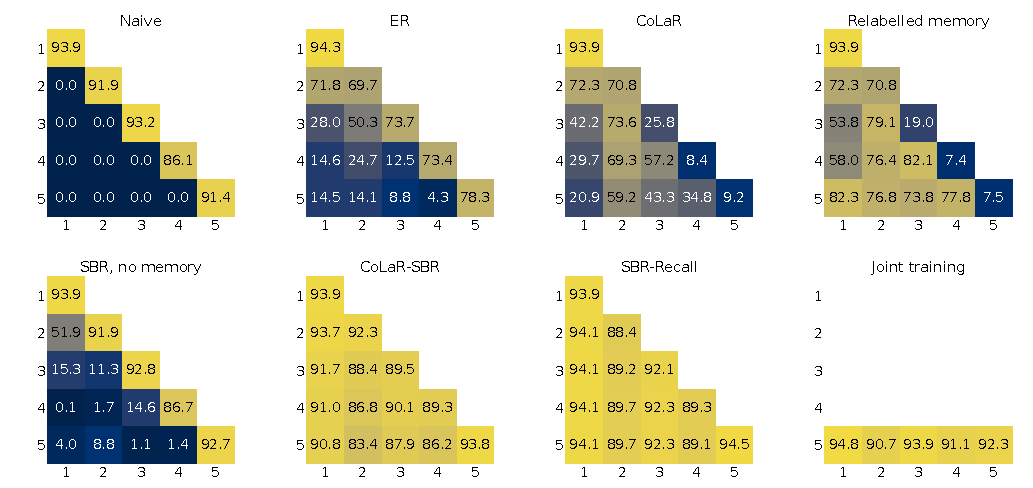
\includegraphics[width=\textwidth]{paper/heatmaps.pdf}
  \caption[Retention matrices on CIL-CORD]{\textbf{Retention matrices} on CIL-CORD
  (session-restricted F1). Row $i$: after training session $i$; column $j$: session $j$.
  Joint training is one pooled run, so only its final row exists.}
  \label{fig:heatmaps}
\end{figure}

\subsection{H2: The Labels Are the Cause}
\label{sec:r-h2}

We next hypothesized that the labels are the cause, on the stored side and on the current
side. If so, repairing the labels should close the gap with the shared softmax unchanged.

\paragraph{Stored side.} We repair the stored labels with the ground-truth labels, which a
continual learner does not have. When every stored document is relabelled \emph{before
each session} with the true labels of all classes in the grown head, the same memory and
the same softmax reach $\vOraclePreFull$ full-label F1, within $\nOraclePreJointGap$ points
of joint training. Masking the stale tokens in the replay loss, which removes the false
background label without adding a label, reaches $\vOracleMaskFull$. Hence, removing the
stale negatives alone recovers most of the gap on this stream. The timing of the repair
matters. When the older stored documents are relabelled only at the session boundaries,
the documents of the session that is being trained are not yet covered, and the repair
helps one session too late: \gls{aa} rises from $\nColarSeed$ to $\nOracle$, but
sessions~3 to~5 are learned only to $\nOracleLateMin$ to $\nOracleLateMax$ F1 on their own
diagonal, sessions~3 and~4 rise to $\nOracleNextMin$ to $\nOracleNextMax$ one session
later, and the last session ends at $\nOracleLast$.

\paragraph{Current side.} We then repair the loss, which needs no additional annotation.
The MiB-style loss of Equation~\eqref{eq:mib} lifts the full-label F1 to $\vMibFull$, i.e.,
$\nMibShareFull\%$ of the gap to joint training. It learns every session to at least
$\nMibDiagMin$ F1; however, the first session ends at no more than $\nMibFirstMax$ F1 in
any run. Slicing the softmax of the replay loss reaches only $\vSlicedFull$, and slicing
both losses, the control inspired by SS-IL, reaches $\vSlicedBothFull$. It is noted that
the sliced variant trains unstably: within a session, its validation F1 can collapse after
its peak. Thus, a repair of the loss helps only partly on CIL-CORD. Besides, the
ground-truth labels above close the gap although every current document still labels old
entities as background; hence, the current side does not prevent this rescue on CIL-CORD.

\paragraph{The other streams.} The picture changes with the stream
(Figure~\ref{fig:repairs}, Table~\ref{tab:repairs}). On CIL-FUNSD, the ground-truth stored
labels leave the shared softmax where it was, whereas the MiB-style loss is level with our
readout. On CIL-WildReceipt, the ground-truth labels help only partly, and the MiB-style
loss stays below our readout. This can be due to the share of the two sides in each stream:
in CIL-FUNSD, the forms of the second session contain the questions of the first one, so
the current side dominates, whereas in CIL-CORD the stored documents carry many stale
labels.

\paragraph{Outcome.} H2 is only partly supported: repairing the labels helps, but no label
repair closes the gap on every stream.

\begin{figure}[!htbp]
  \centering
  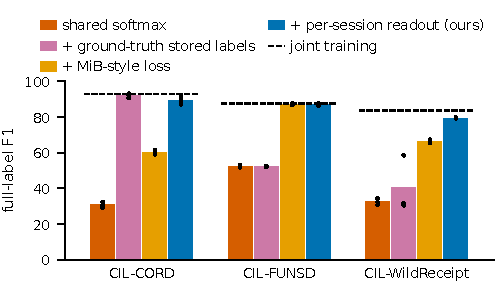
\includegraphics[width=0.62\textwidth]{paper/repairs.pdf}
  \caption[Three repairs on three class-incremental streams]{\textbf{Three repairs on three
  class-incremental streams} (full-label F1; dashed: joint training). Only the per-session
  readout closes most of the gap on all three streams.}
  \label{fig:repairs}
\end{figure}

\begin{table}[!htbp]
  \centering
  \caption[Three repairs on three class-incremental streams: values]{\textbf{Three repairs
  on three class-incremental streams} (full-label F1, mean $\pm$ s.d.). Every row but the
  last uses the same CoLaR memory, and the first three keep the shared softmax. The
  ground-truth stored labels are not available to a continual learner.}
  \label{tab:repairs}
  % AUTO-GENERATED by scripts/rca/make_clean_tables.py -- do not edit.
\begin{tabular}{lccc}
\toprule
Repair & CIL-CORD & CIL-FUNSD & CIL-WildReceipt \\
\midrule
Shared softmax (CoLaR) & $30.7{\pm}1.5$ & $52.2{\pm}0.6$ & $32.5{\pm}1.8$ \\
+ ground-truth stored labels & $92.1{\pm}1.3$ & $52.2{\pm}0.2$ & $40.3{\pm}15.9$ \\
+ MiB-style loss & $60.0{\pm}1.2$ & $87.3{\pm}0.4$ & $66.5{\pm}0.8$ \\
+ per-session readout (CoLaR-SBR) & $89.1{\pm}2.0$ & $87.2{\pm}0.6$ & $79.5{\pm}0.3$ \\
\midrule
Joint training (reference) & $93.1{\pm}1.0$ & $87.5{\pm}0.8$ & $83.7{\pm}1.0$ \\
\bottomrule
\end{tabular}

\end{table}

\subsection{H3: The Shared Normalisation}
\label{sec:r-h3}

Finally, we hypothesized that the conflict lives in the shared normalisation: one
background logit trained by documents that disagree on the background. If so, one
background logit per session, normalised with the tags of that session only, should close
most of the gap without additional annotations.

\paragraph{With the memory.} The hypothesis is supported. With the memory, the blocked
readout (CoLaR-SBR) reaches $\vSbrFull$ full-label F1, $\nSbrGapFullMin$ to
$\nSbrGapFullMax$ points below joint training, and no ground-truth label is used. Every
session is learned when it is trained, and the columns of its retention matrix hold
(Figure~\ref{fig:heatmaps}). Regarding the remaining gap, a session loses $\sbrLossMin$ to
$\sbrLossMax$ points from its diagonal to the final row, session~$\sbrLossMaxSession$ the
most. Hence, what CoLaR-SBR still loses to joint training is the retention of the early
sessions.

\paragraph{Without the memory.} Without the memory, the same readout scores only
$\vNoBankFull$. The reason is not the conflict: no old entity token is predicted as ``O''.
Instead, $\mNoBankOtherMin$ to $\mNoBankOtherMax\%$ of the wrong tokens receive a class of
another session, and each old block claims $\mNoBankFalseMin$ to $\mNoBankFalseMax\%$ of
the tokens of its own test split that are not its entities, against $\mSbrFalseMin$ to
$\mSbrFalseMax\%$ with the memory. This is consistent with an encoder that has drifted
under a readout that no longer fits it. Thus, the readout removes the conflict and the
memory removes the drift; neither replaces the other (Section~\ref{sec:c6-s4}).

\paragraph{Where the entities of old sessions go.} Figure~\ref{fig:findings} summarises
the three hypotheses and shows, for the final model, where the entities of the old sessions
end. Under CoLaR-SBR, the owning block claims $\mSbrOwnerMin$ to $\mSbrOwnerMax\%$ of the
old entity tokens, and most of the remaining errors ($\mSbrSameMin$ to $\mSbrSameMax\%$ of
the wrong tokens) give the token another tag of its own session. Therefore, the blocks
rarely confuse the sessions; what is left is the usual confusion between the classes of
one session. With a shared softmax and a memory, the newest session is suppressed, whereas
naive fine-tuning learns it and keeps nothing older (Figure~\ref{fig:findings}c).

\paragraph{Outcome.} H3 is supported on all three class-incremental streams
(Figure~\ref{fig:repairs}): the label-side repairs each succeed on one stream, whereas the
blocked readout closes most of the gap on all three. This motivates the readout of our
method.

\begin{figure}[!htbp]
  \centering
  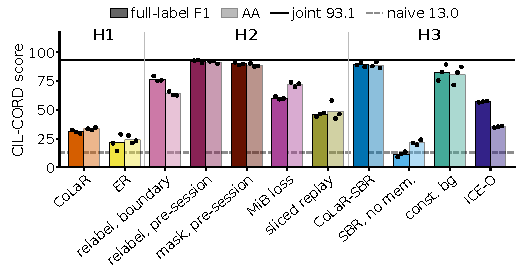
\includegraphics[width=0.56\textwidth]{paper/findings_a.pdf}\hfill
  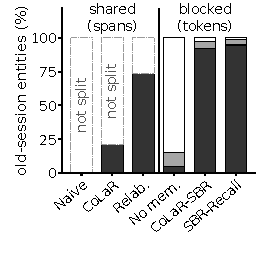
\includegraphics[width=0.21\textwidth]{paper/findings_b.pdf}\hfill
  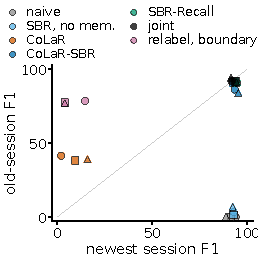
\includegraphics[width=0.21\textwidth]{paper/findings_c.pdf}\\
  \makebox[0.56\textwidth]{\small(a)}\hfill\makebox[0.21\textwidth]{\small(b)}\hfill\makebox[0.21\textwidth]{\small(c)}\\[2pt]
  
\includegraphics[width=0.6\textwidth]{paper/findings_b_key.pdf}
  \caption[The findings on CIL-CORD in one figure]{\textbf{The findings in one figure}
  (CIL-CORD). (a) The series of hypotheses: full-label F1 (dark) and AA (light). (b) Where
  the final model puts the entities of the old sessions. (c) F1 of the newest session
  against the mean F1 of the old sessions, one marker per run.}
  \label{fig:findings}
\end{figure}

\subsection{One Principle behind the Repairs}
\label{sec:r-principle}

The repairs of this section differ in what they change, but they follow one principle: a
stored background label must not count against a class that its document could not
annotate (Table~\ref{tab:scope}). The shared softmax violates it, the slices and the
MiB-style loss weaken the violation, the ground-truth labels remove it with information
that a continual learner does not have, and the per-session readout removes it in the
normalisation. As the results demonstrate, the three repairs that follow the principle fully
(the last three rows) come close to joint training, and the per-session readout is the
only one of them that needs no ground-truth label.

\begin{table}[!htbp]
  \centering
  \caption[One principle, six repairs]{\textbf{One principle, six repairs} (CIL-CORD, same
  CoLaR memory, full-label F1): how each repair treats a stored background label.
  $^{r}$Uses the ground-truth labels.}
  \label{tab:scope}
  \begin{tabular}{@{}llc@{}}
    \toprule
    Repair & Treatment of a stored background label & F1 \\
    \midrule
    Shared softmax & background against all entities & $\vColarFull$ \\
    Softmax slice & background against the entities known at storage & $\vSlicedFull$ \\
    MiB-style loss & marginal target: ``O or a later class'' & $\vMibFull$ \\
    Stale tokens masked$^{r}$ & no loss where the label is stale & $\vOracleMaskFull$ \\
    True stored labels$^{r}$ & corrected to the true label & $\vOraclePreFull$ \\
    Per-session readout (SBR) & background within its own session & $\vSbrFull$ \\
    \bottomrule
  \end{tabular}
\end{table}

% =============================================================================
\section{Main Comparison on Six Streams}
\label{sec:c6-s3}

The results on the six streams are shown in Table~\ref{tab:main}. Overall, naive
fine-tuning forgets heavily on every stream but DIL-XFUND, and no baseline with a shared
softmax comes close to joint training on the class-incremental streams. In contrast,
CoLaR-SBR or its memory-free variant achieves the best result on the three
class-incremental streams and on Mixed.

\begin{landscape}
\begin{table}[p]
  \centering
  \caption[Comparison with the baselines on six streams]{\textbf{Comparison with
  continual-learning baselines} on six streams. F1: full-label F1; AA and AF: average
  accuracy and forgetting. AA and F1: mean $\pm$ s.d.; AF: mean; ``--'': not applicable.
  Bold: best AA and F1 of each column, joint training aside; underlined: our best when a
  baseline is best. $^{b}$With the $50$-document memory.}
  \label{tab:main}
  \resizebox{\linewidth}{!}{% AUTO-GENERATED by scripts/rca/make_clean_tables.py -- do not edit.
\begin{tabular}{@{}llccccccccccccc@{}}
\toprule
 & & \multicolumn{3}{c}{CIL-CORD} & \multicolumn{2}{c}{Mixed} & \multicolumn{2}{c}{DIL} & \multicolumn{2}{c}{CIL-FUNSD} & \multicolumn{2}{c}{CIL-WildReceipt} & \multicolumn{2}{c}{DIL-XFUND} \\
\cmidrule(lr){3-5}\cmidrule(lr){6-7}\cmidrule(lr){8-9}\cmidrule(lr){10-11}\cmidrule(lr){12-13}\cmidrule(l){14-15}
Family & Method & F1$\uparrow$ & AA$\uparrow$ & AF$\downarrow$ & AA$\uparrow$ & AF$\downarrow$ & AA$\uparrow$ & AF$\downarrow$ & AA$\uparrow$ & AF$\downarrow$ & AA$\uparrow$ & AF$\downarrow$ & AA$\uparrow$ & AF$\downarrow$ \\
\midrule
Reference & Naive fine-tuning & $13.0{\pm}0.2$ & $18.3{\pm}0.5$ & $91.3$ & $42.1{\pm}0.7$ & $54.6$ & $39.2{\pm}0.3$ & $71.7$ & $43.9{\pm}0.5$ & $86.1$ & $19.6{\pm}0.1$ & $82.7$ & $71.2{\pm}0.7$ & $7.5$ \\
 & Joint training & $93.1{\pm}1.0$ & $92.6{\pm}0.9$ & -- & $87.6{\pm}0.7$ & -- & $86.7{\pm}0.2$ & -- & $87.9{\pm}0.7$ & -- & $83.5{\pm}0.8$ & -- & $79.5{\pm}0.4$ & -- \\
\midrule
Regularisation & LwF (2016) & $13.0{\pm}0.4$ & $18.5{\pm}0.6$ & $90.5$ & $44.2{\pm}1.4$ & $52.8$ & $37.6{\pm}1.1$ & $73.7$ & $44.0{\pm}0.3$ & $84.4$ & $19.8{\pm}0.3$ & $82.5$ & $72.0{\pm}0.2$ & $4.8$ \\
\midrule
Replay & ER (2019) & $21.2{\pm}7.3$ & $24.0{\pm}3.4$ & $67.4$ & $76.4{\pm}3.3$ & $6.9$ & $87.0{\pm}0.2$ & $0.1$ & $47.4{\pm}3.9$ & $72.0$ & $20.3{\pm}0.4$ & $77.7$ & $79.3{\pm}1.0$ & $-2.4$ \\
 & DER++ (2020) & $18.6{\pm}6.4$ & $21.2{\pm}1.6$ & $82.5$ & $73.7{\pm}4.6$ & $18.1$ & $\mathbf{88.2{\pm}1.8}$ & $2.5$ & $46.6{\pm}6.2$ & $75.2$ & $19.7{\pm}0.7$ & $81.3$ & $\mathbf{80.2{\pm}0.3}$ & $-1.0$ \\
\midrule
Prompt, LoRA & CODA-Prompt (2023) & $5.6{\pm}3.8$ & $7.3{\pm}4.7$ & $28.6$ & $8.5{\pm}0.8$ & $33.7$ & $31.0{\pm}0.2$ & $35.4$ & $10.0{\pm}6.5$ & $17.3$ & $14.0{\pm}0.1$ & $68.3$ & $30.9{\pm}0.3$ & $-3.7$ \\
 & CL-LoRA (2025) & $12.8{\pm}0.6$ & $18.4{\pm}0.6$ & $73.8$ & $41.3{\pm}0.4$ & $51.1$ & $42.5{\pm}0.8$ & $60.6$ & $41.2{\pm}1.2$ & $79.0$ & $18.2{\pm}0.4$ & $78.0$ & $53.6{\pm}5.2$ & $9.3$ \\
\midrule
Continual NER & CPFD (2023) & $4.5{\pm}6.7$ & $6.3{\pm}10.6$ & $30.2$ & $2.0{\pm}3.5$ & $38.7$ & $0.0{\pm}0.0$ & $56.2$ & $23.3{\pm}21.1$ & $79.6$ & $7.8{\pm}9.9$ & $26.7$ & $1.8{\pm}3.2$ & $39.9$ \\
 & IS3 (2024) & $8.7{\pm}1.2$ & $5.2{\pm}1.5$ & $43.8$ & $14.0{\pm}24.3$ & $39.6$ & $38.4{\pm}0.3$ & $37.4$ & $27.0{\pm}0.2$ & $83.9$ & $4.1{\pm}0.1$ & $39.0$ & $64.7{\pm}1.4$ & $8.0$ \\
\midrule
Merging & LCA (2026) & $10.9{\pm}0.7$ & $8.8{\pm}1.2$ & $56.4$ & $33.9{\pm}7.1$ & $26.9$ & $41.1{\pm}2.6$ & $30.2$ & $56.6{\pm}4.3$ & $35.4$ & $32.1{\pm}7.5$ & $40.3$ & $65.1{\pm}1.3$ & $-0.3$ \\
\midrule
\rowcolor{black!7}Ours & CoLaR (memory only) & $30.7{\pm}1.5$ & $33.5{\pm}1.0$ & $10.2$ & $74.7{\pm}6.8$ & $11.3$ & $\underline{86.5{\pm}0.7}$ & $0.7$ & $45.0{\pm}0.2$ & $85.8$ & $22.8{\pm}4.8$ & $57.5$ & $\underline{76.9{\pm}1.6}$ & $-1.9$ \\
\rowcolor{black!7} & CoLaR-SBR & $89.1{\pm}2.0$ & $88.4{\pm}2.6$ & $4.2$ & $\mathbf{89.1{\pm}0.6}$ & $-0.1$ & $85.4{\pm}0.4$ & $3.7$ & $87.4{\pm}0.6$ & $-1.4$ & $79.4{\pm}0.3$ & $1.6$ & $76.4{\pm}0.5$ & $-2.4$ \\
\rowcolor{black!7} & SBR-Recall & $\mathbf{92.6{\pm}1.0}$ & $\mathbf{91.9{\pm}0.6}$ & $-0.4$ & $84.8{\pm}1.0^{b}$ & $3.5$ & $31.8{\pm}1.7$ & $37.4$ & $\mathbf{87.6{\pm}1.7}$ & $0.1$ & $\mathbf{81.1{\pm}0.4}$ & $-0.2$ & $52.1{\pm}3.5$ & $8.6$ \\
\bottomrule
\end{tabular}
}
\end{table}
\end{landscape}

\paragraph{Results on the class-incremental streams.} On CIL-CORD, CoLaR-SBR achieves
$\vSbrFull$ full-label F1 ($\vSbr$ AA), which significantly improves over the same memory
with a shared softmax ($\vColarFull$) and comes close to the upper-bound baseline, joint
training ($\vJointFull$). Our method also surpasses the other baselines by a large margin:
the best of them, ER with $\nErCilBuf$ raw documents, reaches only $\vErFull$.
Interestingly, the continual NER methods CPFD and IS3, which are designed for the shift of
the background label, do not benefit either; this can be due to the shared softmax that
they keep. On top of that, SBR-Recall gains the highest
score ($\vRecallFull$) with no stored document. We observe the same pattern on the two
other class-incremental streams. On CIL-FUNSD, CoLaR-SBR reaches $\vFunsdSbr$ AA, level
with joint training ($\vFunsdJoint$), whereas CoLaR with a shared softmax stays close to
naive fine-tuning ($\vFunsdColar$ against $\vFunsdNaive$). On CIL-WildReceipt, CoLaR-SBR
reaches $\vWildSbr$ AA against $\vWildColar$ for the shared softmax; nevertheless, our
method still has a gap to joint training there ($\vWildJoint$).

\paragraph{Results on the domain-incremental streams.} On a fixed label space there is one
block and nothing to separate; hence, these streams test the memory alone. On DIL, naive
fine-tuning reaches only $\vNaiveDil$ AA against $\vJointDil$ for joint training, whereas
every replay method comes close to joint training (ER: $\vErDil$, CoLaR: $\vColarDil$,
CoLaR-SBR: $\vSbrDil$). Thus, it is reasonable that the blocked readout brings no gain
here. On DIL-XFUND, where only the language changes, forgetting is milder ($\vXfundNaive$
for naive fine-tuning against $\vXfundJoint$ for joint training). CoLaR and CoLaR-SBR
improve over naive fine-tuning ($\vXfundColar$ and $\vXfundSbr$), but they stay below ER
and DER++ ($\vXfundEr$ and $\vXfundDerPp$), which keep raw documents and train every
layer. This hints that the frozen lower layers limit the adaptation to a new language, in
particular to a new script. As predicted in Section~\ref{sec:m-recall}, SBR-Recall, which
has no memory and nothing to select its states by on a fixed label space, falls below
naive fine-tuning on both streams ($\vRecallDil$ on DIL).

\paragraph{Results on the Mixed stream.} On Mixed, the sessions change the classes, the
domain and the annotation schema. Naive fine-tuning reaches $\vNaiveMix$ AA. A memory
under a shared softmax helps (ER: $\vErMix$, CoLaR: $\vColarMix$), but it leaves a gap to
joint training ($\vJointMix$). In contrast, CoLaR-SBR gains the highest \gls{aa} among all
methods ($\vSbrMix$), on par with joint training and with almost no forgetting. SBR-Recall
needs the memory on this stream: it reaches $\nRecallMixMem$ AA with the $50$-document
memory and only $\nRecallMixNoMem$ without it.

\paragraph{Forgetting analysis.} Figure~\ref{fig:forgetting} follows the F1 over the
sessions of CIL-CORD. After the five sessions, naive fine-tuning keeps $\nFirstNaive$ F1
on session~1 and CoLaR with a shared softmax $\nFirstColar$, whereas CoLaR-SBR keeps
$\nFirstSbr$ and SBR-Recall $\nFirstRecall$. CoLaR-SBR and SBR-Recall stay close to joint
training after every session, whereas the methods with a shared softmax lose session~1
step by step. It is noted that CoLaR with a shared softmax has a low \gls{af} only because
it suppresses each new session while learning it; hence, \gls{af} must be read together
with \gls{aa} and with the diagonal of the retention matrix.

\begin{figure}[!htbp]
  \centering
  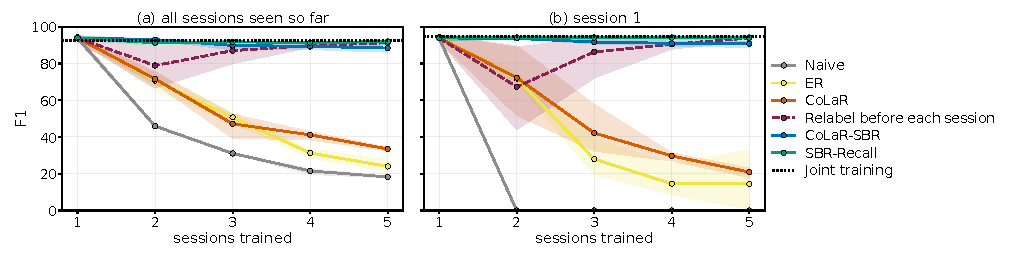
\includegraphics[width=\textwidth]{paper/forgetting.pdf}
  \caption[Forgetting on CIL-CORD]{\textbf{Forgetting on CIL-CORD}, session by session
  (line: mean of three runs, band: their range). (a) F1 averaged over the sessions seen so
  far. (b) F1 of session~1.}
  \label{fig:forgetting}
\end{figure}

% =============================================================================
\section{Component Ablation}
\label{sec:c6-s4}

To assess the contribution of each component of CoLaR-SBR, we conduct an ablation study on
CIL-CORD (Table~\ref{tab:components}). Starting from naive fine-tuning (Index~I), we add
the CoLaR memory, the session-blocked readout and the learned background logit.

\begin{table}[!htbp]
  \centering
  \caption[Ablation study of CoLaR-SBR]{\textbf{Ablation study of CoLaR-SBR} on CIL-CORD
  (F1: full-label F1; mean $\pm$ s.d.). Rows I to V add the components; rows VI and VII
  replace the latent memory with raw documents and with per-session updates (SBR-Recall).
  Bold: the full CoLaR-SBR.}
  \label{tab:components}
  % AUTO-GENERATED by scripts/rca/make_clean_tables.py -- do not edit.
\begin{tabular}{@{}lccc ccc@{}}
\toprule
Index & Memory & Blocked readout & Learned bg. & F1$\uparrow$ & AA$\uparrow$ & AF$\downarrow$ \\
\midrule
I & -- & -- & -- & $13.0{\pm}0.2$ & $18.3{\pm}0.5$ & $91.3$ \\
II & \checkmark & -- & -- & $30.7{\pm}1.5$ & $33.5{\pm}1.0$ & $10.2$ \\
III & -- & \checkmark & \checkmark & $11.4{\pm}2.3$ & $21.6{\pm}2.2$ & $87.5$ \\
IV & \checkmark & \checkmark & -- & $82.4{\pm}6.9$ & $80.2{\pm}8.1$ & $0.2$ \\
V & \checkmark & \checkmark & \checkmark & $\mathbf{89.1{\pm}2.0}$ & $\mathbf{88.4{\pm}2.6}$ & $4.2$ \\
\midrule
VI & raw & \checkmark & \checkmark & $88.4{\pm}1.0$ & $88.4{\pm}1.1$ & $5.2$ \\
VII & deltas & \checkmark & \checkmark & $92.6{\pm}1.0$ & $91.9{\pm}0.6$ & $-0.4$ \\
\midrule
\multicolumn{4}{@{}l}{Joint training (reference)} & $93.1{\pm}1.0$ & $92.6{\pm}0.9$ & -- \\
\bottomrule
\end{tabular}

\end{table}

The baseline (I) forgets almost everything. The memory alone (II) lifts the full-label F1
by only $\nAblMemGain$ points, since the shared softmax still counts every background
label against all classes. The readout alone (III) does not help either
($\nAblReadAlone$), because the old blocks drift without a memory. Notably, adding the
blocked readout to the memory (IV) yields the most substantial boost ($\nAblReadoutGain$
points over II). Finally, the learned background logit (V) further improves the result by
$\nAblBgGain$ points. Overall, the complete CoLaR-SBR surpasses naive fine-tuning by
$\nAblFullGain$ points, far more than the memory and the readout add up to on their own,
which confirms that they address two different causes.

\paragraph{Memory format.} Our readout is not limited to the latent memory: with raw
documents (VI), it reaches $\vErSbrFull$ against $\vSbrFull$. Hence, the readout carries
the gain, and the format of the memory is a matter of cost. We keep the latent memory
because it stores no pixels or token ids and trains only $\nMemTrainSbrPct\%$ of the
parameters that raw replay trains (Section~\ref{sec:c6-s7}).

\paragraph{Memory-free variant.} SBR-Recall (VII) replaces the memory with per-session
low-rank updates and reaches $\vRecallFull$ full-label F1, within $\nRecallJointGap$
points of joint training. Under SBR-Recall, the owning block claims $\mRecallOwnerMin$ to
$\mRecallOwnerMax\%$ of the old entity tokens, and every session ends within
$\recallDevMax$ points of its diagonal, since its state is never changed. However, on
Mixed and on the domain-incremental streams it needs the memory
(Section~\ref{sec:c6-s3}). Hence, the updates replace the memory only when the classes grow
within one schema.

% =============================================================================
\section{Analysis of the Settings}
\label{sec:c6-s5}

In this section, we study the impact of each setting of CoLaR-SBR on CIL-CORD. We change
one setting at a time around the default, i.e., $50$ documents per session, rank $128$,
injection at layer~$4$ and four replayed documents per batch.

\paragraph{Impact of the memory size.} We vary the number of stored documents per session
from $5$ to $200$ (Figure~\ref{fig:budget}, Table~\ref{tab:budget}). CoLaR-SBR needs a
memory of sufficient size. With $5$ documents it reaches only $\nBudSbrFive$ full-label
F1, and with $10$ documents it is unstable (from $\nBudSbrTenLo$ to $\nBudSbrTenHi$
between runs). The performance then improves quickly ($\nBudSbrTwenty$ with $20$,
$\nBudSbrThirty$ with $30$, $\nBudSbrForty$ with $40$ and $\nBudSbrFifty$ with $50$).
Beyond that, the improvement is small ($\nBudSbrHundred$ with $100$, $\nBudSbrTwoHundred$
with $200$). In contrast, the shared softmax stays far below at every size: it reaches
$\nBudColarHundred$ with $100$ documents and $\nBudColarTwoHundred$ with $200$, against
$\nBudColarFifty$ with $50$, and its runs spread more as the memory grows. Hence, a larger
memory alone does not close the gap under label growth, which is the last piece of evidence
against H1, and we use $50$ documents per session.

\begin{figure}[!htbp]
  \centering
  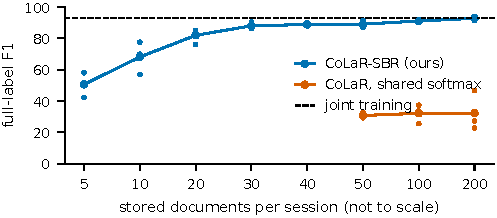
\includegraphics[width=0.6\textwidth]{paper/budget.pdf}
  \caption[Impact of the memory size]{\textbf{Impact of the memory size} on CIL-CORD:
  full-label F1 against stored documents per session (dots: runs; line: their mean; dashed:
  joint training).}
  \label{fig:budget}
\end{figure}

\begin{table}[!htbp]
  \centering
  \caption[Memory size on CIL-CORD: values]{\textbf{Memory size} on CIL-CORD (mean $\pm$
  s.d.; bold: the default size).}
  \label{tab:budget}
  % AUTO-GENERATED by scripts/rca/make_clean_tables.py -- do not edit.
\begin{tabular}{@{}lrcc@{}}
\toprule
Readout & Documents per session & Full-label F1 & AA \\
\midrule
Per-session (CoLaR-SBR) & 5 & $50.6{\pm}7.9$ & $59.9{\pm}3.6$ \\
 & 10 & $68.1{\pm}10.4$ & $73.8{\pm}3.4$ \\
 & 20 & $81.9{\pm}5.1$ & $84.0{\pm}2.3$ \\
 & 30 & $88.0{\pm}2.1$ & $86.0{\pm}2.8$ \\
 & 40 & $88.9{\pm}1.1$ & $87.6{\pm}1.8$ \\
 & \textbf{50} & $89.1{\pm}2.0$ & $88.4{\pm}2.6$ \\
 & 100 & $91.1{\pm}0.9$ & $90.1{\pm}1.0$ \\
 & 200 & $92.8{\pm}1.3$ & $92.7{\pm}1.0$ \\
\midrule
Shared softmax (CoLaR) & \textbf{50} & $30.7{\pm}1.5$ & $33.5{\pm}1.0$ \\
 & 100 & $32.1{\pm}6.0$ & $27.7{\pm}7.4$ \\
 & 200 & $32.2{\pm}12.7$ & $31.0{\pm}6.0$ \\
\bottomrule
\end{tabular}

\end{table}

\paragraph{Impact of the SVD rank.} The rank decides how faithfully a stored document is
kept (Table~\ref{tab:analysis}). As the results demonstrate, a smaller rank hurts our
method: at rank $64$, CoLaR-SBR falls to $\vSbrRankSixtyFourFull$ full-label F1 and becomes
unstable, and at rank $32$ it falls to $\vSbrRankThirtyTwoFull$, i.e.,
$\nSbrRankThirtyTwoDropMin$ to $\nSbrRankThirtyTwoDropMax$ points below rank $128$. This
indicates the importance of keeping the whole document faithfully. Thus, it is suggested
that a rank of $128$ ensures decent performance.

\paragraph{Impact of the injection layer.} The layer $k$ decides how many layers are
frozen and how many are trained on the stored documents. With $k=2$, $6$ or $8$, CoLaR-SBR
stays between $\nAnaLayerLo$ and $\nAnaLayerHi$ full-label F1, against $\vSbrFull$ with
$k=4$. Hence, our method is not sensitive to this setting, and we keep $k=4$.

\paragraph{Impact of the replayed documents per batch.} We replay two, four or eight
stored documents with each batch of two current documents. The results stay between
$\nAnaReplayLo$ and $\nAnaReplayHi$ full-label F1. Hence, our method is not sensitive to
this setting either, and we keep four replayed documents.

\begin{table}[!htbp]
  \centering
  \caption[Settings of CoLaR-SBR]{\textbf{Settings of CoLaR-SBR} on CIL-CORD: one setting
  changes at a time (bold: the default; mean $\pm$ s.d.).}
  \label{tab:analysis}
  % AUTO-GENERATED by scripts/rca/make_clean_tables.py -- do not edit.
\begin{tabular}{@{}lccc@{}}
\toprule
Setting & Value & Full-label F1 & AA \\
\midrule
SVD rank & 32 & $27.4{\pm}2.5$ & $33.1{\pm}2.5$ \\
 & 64 & $79.4{\pm}16.5$ & $81.4{\pm}12.9$ \\
 & \textbf{128} & $89.1{\pm}2.0$ & $88.4{\pm}2.6$ \\
\midrule
Injection layer $k$ & 2 & $88.7{\pm}1.1$ & $87.6{\pm}2.4$ \\
 & \textbf{4} & $89.1{\pm}2.0$ & $88.4{\pm}2.6$ \\
 & 6 & $90.6{\pm}1.8$ & $89.0{\pm}1.8$ \\
 & 8 & $88.1{\pm}2.0$ & $84.7{\pm}2.7$ \\
\midrule
Replayed documents per batch & 2 & $90.0{\pm}1.1$ & $89.3{\pm}1.9$ \\
 & \textbf{4} & $89.1{\pm}2.0$ & $88.4{\pm}2.6$ \\
 & 8 & $90.2{\pm}2.2$ & $89.0{\pm}2.8$ \\
\bottomrule
\end{tabular}

\end{table}

\section{Robustness}
\label{sec:c6-s6}
% SOURCE: session order, BROS + E2 encoders, patience
\todo{to be written}

\section{Memory and Computational Cost}
\label{sec:c6-s7}
% SOURCE: paper App. B memory analysis; E6 cost table
\todo{to be written}

\section{Beyond Documents: Image Classification}
\label{sec:c6-s8}
% SOURCE: paper App. F; E4
\todo{to be written}

\section{Qualitative and Error Analysis}
\label{sec:c6-s9}
% SOURCE: receipt figure, per-class results, where the owner block errs
\todo{to be written}

\section{Discussion}
\label{sec:c6-s10}
% SOURCE: answers to RQ1-RQ4; relation to prior work
\todo{to be written}


% Chapter 7 (two-cause rewrite, 2026-11). Result numbers are generated macros.
% Old text: chapters_old/chapter7.tex (git tag thesis-pre-two-causes).
\chapter{Conclusions and Future Work}
\label{ch:conclusion}

\section{Conclusions}
\label{sec:c7-s1}

In this thesis, we investigated why key-information extraction models forget when
documents and labels arrive in sequence, and we proposed a novel method called CoLaR-SBR.
We answer the four research questions of Section~\ref{sec:c1-s3} as follows.

\paragraph{RQ1: What causes forgetting in continual \gls{kie}?} Two causes. The first is
the drift of the representation: under naive fine-tuning, the features of all four
encoders change, more so with depth, and the head that was fitted on the old features is
displaced the most. Replay removes this cause on a fixed label space, whereas
regularisation does not. The second is the conflict on the background label: when the
label set grows, the stored documents and the current documents each label the entities
of the other sessions as background, and a shared softmax counts every such label against
the class that it hides. A memory does not remove this cause: on CIL-CORD, the memory
alone reaches only $\vColarFull$ full-label F1 against $\vJointFull$ for joint training,
and a larger memory does not close the gap.

\paragraph{RQ2: What must a memory keep?} Whole documents, kept faithfully, but not their
pixels or their token ids. A memory of compressed layer-$4$ activations of $50$ documents
per session is close to raw replay on the domain-incremental stream and, under our
readout, within $\nErSbrAbsFullMax$ full-label F1 points of raw replay on CIL-CORD, while
it trains only $\nMemTrainSbrPct\%$ of the parameters. The fidelity matters more than the
size: a lower rank makes the method unstable, whereas the number of documents saturates
early.

\paragraph{RQ3: How can the background conflict be resolved without additional
annotations?} By normalising each session separately. A repair of the labels closes the
gap on one stream each, and the best of them needs the ground-truth labels. In contrast,
the session-blocked readout, with one learned background per session and a supervision
rule that lets a background label train only the blocks that its document could annotate,
closes most of the gap on all three class-incremental streams with the labels that each
session provides. On CIL-CORD, CoLaR-SBR reaches $\vSbrFull$ full-label F1, and its
memory-free variant SBR-Recall reaches $\vRecallFull$, within $\nRecallJointGap$ points of
joint training.

\paragraph{RQ4: How far does the result hold?} The gap between the shared softmax and the
per-session readout holds on three class-incremental streams, under three session orders
and on a second encoder, and it is not explained by the patience of the baselines or by
the choice of the test documents. On the Mixed stream, CoLaR-SBR is on par with joint
training. The result has limits as well: on the domain-incremental streams the readout
brings nothing, as expected, SBR-Recall needs the memory when the schema changes and
depends on its first session, and on images the choice of the session becomes the main
source of error.

Overall, the experiments show that the memory and the readout address two different causes
and are both needed, and that our method achieves significant improvement over eight
continual-learning baselines on the class-incremental streams of five public document
datasets.

\section{Limitations}
\label{sec:c7-s2}

Our study has several limitations. We state each one with a way forward.

\paragraph{Session information at training time.} The readout opens one block per session
and needs to know, for every training and stored document, which session annotated it. No
such information is needed at test time. In a real stream, the boundaries can be taken
from the change of the label set; detecting them when the schema changes silently is left
open.

\paragraph{Growth with the number of sessions.} The memory grows by a fixed number of
documents per session, and SBR-Recall adds one update and one forward pass per session.
Our streams hold at most a handful of sessions. For longer streams, a memory of fixed
total size and a merging of old updates are natural next steps.

\paragraph{Remaining gaps.} On CIL-WildReceipt, CoLaR-SBR stays below joint training
($\vWildSbr$ against $\vWildJoint$ \gls{aa}), and on DIL-XFUND it stays below raw replay
($\vXfundSbr$ against $\vXfundEr$), which hints that the frozen lower layers limit the
adaptation to a new language. Training the lower layers slowly instead of freezing them,
as in latent replay for devices~\citep{pellegrini2020latent}, is the first thing to try.

\paragraph{The memory-free variant.} SBR-Recall replaces the memory only when the classes
grow within one schema. Besides, it depends on its first session: in one of three runs
under the reversed session order, the first session was not learned, and no later session
recovered. A longer patience for the first session, or a first session trained with
several restarts, may remove this failure.

\paragraph{Encoders and tasks.} Most results are on LayoutLMv3, with one stream on BROS.
We study \gls{kie} as token labelling only; generative document models and multimodal
language models, which produce the fields as text, have no background label in this form,
and whether a related conflict exists for them is unknown.

\paragraph{Privacy.} The latent memory stores no pixels and no token ids. However, we make
no privacy claim, since activations can still leak content; a study of what can be
reconstructed from the stored factors is needed before the memory is used on sensitive
documents.

\section{Future Work}
\label{sec:c7-s3}

Our work is a first step toward continual \gls{kie} that addresses each cause of forgetting
on its own. In the future, we wish to extend it in four directions. First, we will examine
longer streams with dozens of sessions and with recurring schemas, where the number of
blocks and the size of the memory must be bounded. Second, we will study a calibrated
choice of the session for inputs without a background label, which is what limits the
readout on images. Third, we will extend the analysis to generative document models and
multimodal language models, where forgetting after fine-tuning has been
reported~\citep{zhai2023investigating}, and to other extraction tasks such as relation
extraction. Lastly, we will study the privacy of the latent memory, i.e., how much of a
document can be recovered from its compressed activations, and whether the compression can
be designed to prevent it.


% ---- Bibliography ----
\clearpage
\bibliography{refs}
\addcontentsline{toc}{chapter}{References}
\bibliographystyle{plainnat}

% ---- Appendices ----
\begin{appendices}
% Appendix A (two-cause rewrite, 2026-11): settings and baselines. Settings are not results;
% the baseline tables are generated.
\chapter{Settings and Baselines}
\label{app:supplementary}

\section{Training Settings}
\label{app:hyperparameters}

Table~\ref{tab:hyperparameters} lists the settings shared by all runs and the settings of
our method. The protocol is described in Section~\ref{sec:e-protocol}.

\begin{table}[!htbp]
  \centering
  \caption[Training settings]{\textbf{Training settings.} Top: shared by all methods.
  Bottom: the proposed method.}
  \label{tab:hyperparameters}
  \small
  \begin{tabular}{@{}l >{\raggedright\arraybackslash}p{9.6cm}@{}}
    \toprule
    Setting & Value \\
    \midrule
    \multicolumn{2}{@{}l}{\emph{Shared}} \\
    Main encoder & LayoutLMv3-base ($12$ layers, width $768$) \\
    Optimiser & AdamW, learning rate $5\times10^{-5}$, weight decay $0.01$ \\
    Gradient clipping & norm $1.0$ \\
    Batch size & $2$ documents, gradient checkpointing \\
    Precision & full precision \\
    Epochs per session & at most $10$ ($100$ for joint training) \\
    Early stopping & $10\%$ of the session held out; patience $2$ epochs; minimum gain $0.1$ F1 \\
    Input & $512$ tokens, $224\times224$ image, boxes in $[0,1000]$ \\
    Runs per cell & $3$ \\
    \midrule
    \multicolumn{2}{@{}l}{\emph{CoLaR-SBR}} \\
    Injection layer $k$ & $4$ (layers $1$ to $4$ frozen after the first session) \\
    Rank $r$ of the stored factors & $128$, half precision \\
    Stored documents & $50$ per session ($10$ on CIL-FUNSD) \\
    Replayed documents per batch & $4$ \\
    Claim threshold & $0.5$ \\
    \midrule
    \multicolumn{2}{@{}l}{\emph{SBR-Recall}} \\
    Rank of an update & $64$, scale $\alpha=128$ \\
    Updated maps & query, key, value, attention output and both feed-forward maps of layers $5$ to $12$ \\
    Stored documents & none on one schema; $50$ per session across schemas \\
    \bottomrule
  \end{tabular}
\end{table}

\section{Baselines}
\label{app:baselines}

Table~\ref{tab:baselinecard-full} gives the full card of the eight baselines: what our
re-implementation keeps from the published method, what it changes, and what it keeps
across the sessions. Table~\ref{tab:baseline-hp} lists their hyper-parameters as recorded
by the runs; they are the defaults of each method. LCA keeps its published optimiser
instead of AdamW, i.e., SGD with momentum.

\begin{landscape}
\begin{table}[p]
  \centering
  \caption[Baseline card]{\textbf{Baseline card}: the published method, what our
  re-implementation keeps and changes, and its memory on CIL-CORD.}
  \label{tab:baselinecard-full}
  \resizebox{\linewidth}{!}{% AUTO-GENERATED by scripts/rca/make_clean_tables.py -- do not edit.
\begin{tabular}{@{}lll>{\raggedright\arraybackslash}p{4.0cm}>{\raggedright\arraybackslash}p{4.6cm}>{\raggedright\arraybackslash}p{2.6cm}@{}}
\toprule
Method & Venue & Family & Kept from the method & Changed in our version & Memory \\
\midrule
ER & NeurIPS 2019 & Replay & reservoir buffer replayed in every step & -- & 250 raw documents \\
DER++ & NeurIPS 2020 & Replay & replay of documents with labels and stored logits & -- & 250 raw documents + logits \\
LwF & ECCV 2016 & Regularisation & distillation of the old logits towards the previous model & -- & previous model \\
CODA-Prompt & CVPR 2023 & Prompt, LoRA & attention-weighted prompt components with an orthogonality penalty, frozen encoder & prompts prepended to the input sequence (an input-prepend variant) & none (prompt pool) \\
CL-LoRA & CVPR 2025 & Prompt, LoRA & orthogonality penalty, distillation towards the previous model & one shared rank-8 adapter retrained each session (published: random-orthogonal shared and block-wise task-specific adapters, early-exit distillation); gradient reassignment at scale 1, i.e.\ off & previous model, past adapter matrices \\
CPFD & EMNLP 2023 & Continual NER & confidence pseudo-labels, logit and attention-map distillation, adaptive CE factor & one growing token head (published: per-task classifiers); sample weights set to 1 & previous model \\
IS3 & Findings ACL 2024 & Continual NER & distillation on ``O'' tokens, head-row gradient surgery, prototype replay & one growing token head (published: per-task classifiers) & previous model, class prototypes \\
LCA & ICLR 2026 & Merging & per-session fine-tuning (SGD), TIES backbone merge, Gaussian classifier realignment & one growing token head (published: per-task heads); Gaussians per token class, ``O'' excluded & base and per-session backbones, class Gaussians \\
\bottomrule
\end{tabular}
}
\end{table}
\end{landscape}

\begin{table}[!htbp]
  \centering
  \caption[Hyper-parameters of the baselines]{\textbf{Hyper-parameters of the baselines}
  as recorded by the runs on CIL-CORD. The last three columns give the protocol and the
  number of runs per stream (clean: the protocol of Section~\ref{sec:e-protocol}).}
  \label{tab:baseline-hp}
  \resizebox{\textwidth}{!}{% AUTO-GENERATED by scripts/rca/make_clean_tables.py -- do not edit.
\begin{tabular}{@{}l>{\raggedright\arraybackslash}p{9.6cm}ccc@{}}
\toprule
 & & \multicolumn{3}{c}{Protocol, seeds} \\
\cmidrule(l){3-5}
Method & Hyper-parameters (recorded, CIL-CORD) & CIL-CORD & Mixed & DIL \\
\midrule
ER & buffer\_size 250, replay\_batch\_size 8, epochs 10 & clean, 3 & clean, 3 & clean, 3 \\
DER++ & buffer\_size 250, alpha 0.5, beta 0.5, epochs 10 & clean, 3 & clean, 3 & clean, 3 \\
LwF & alpha 1.0, temperature 2.0, epochs 10 & clean, 3 & clean, 3 & clean, 3 \\
CODA-Prompt & n\_components 10, prompt\_length 5, lambda\_ortho 0.1, epochs 10 & clean, 3 & clean, 3 & clean, 3 \\
CL-LoRA & lora\_rank 8, lora\_alpha 16, lambda\_ortho 0.5, kd\_alpha 1.0, temperature 2.0, shared\_grad\_scale 1.0, epochs 10 & clean, 3 & clean, 3 & clean, 3 \\
CPFD & distill\_weight 2.0, threshold 0.001, epochs 10 & clean, 3 & clean, 3 & clean, 3 \\
IS3 & kd\_weight 2.0, proto\_weight 0.1, grad\_weight 0.6, epochs 10 & clean, 3 & clean, 3 & clean, 3 \\
LCA & lr 0.01, merge\_method ties, merge\_topk 100, ca\_epochs 10, ca\_samples\_per\_cls 256, epochs 10 & clean, 3 & clean, 3 & clean, 3 \\
\bottomrule
\end{tabular}
}
\end{table}

\paragraph{Choice of the baselines.} We fixed the set of baselines after a first comparison
on CIL-CORD, Mixed and DIL. EWC~\citep{kirkpatrick2017ewc}, L2P~\citep{wang2022l2p} and
DualPrompt~\citep{wang2022dualprompt} did not learn sessions~4 and~5 of CIL-CORD in any
run (Table~\ref{tab:dropped}); hence, we dropped them. CPFD and IS3 also fail on this
stream; however, we kept them because they are designed for the shift of the background
label. It is noted that the baselines differ in what they learn as well as in what they
forget: CPFD reaches $\nCpfdLateMax$ F1 on its best later session right after it is
learned, whereas IS3, CODA-Prompt and LCA each have a later session that is learned to at
most $\nBaseWorstLateMax$ F1 in every run. In contrast, naive fine-tuning learns every
session to at least $\nNaiveDiagMin$.

\begin{table}[!htbp]
  \centering
  \caption[Baselines that were dropped]{\textbf{Baselines that were dropped} (CIL-CORD,
  first comparison, earlier protocol; AA per run). Unlearned sessions: the sessions whose
  F1 right after training stays near zero.}
  \label{tab:dropped}
  \small% AUTO-GENERATED by scripts/rca/make_clean_tables.py -- do not edit.
\begin{tabular}{lcccc}
\toprule
 & \multicolumn{3}{c}{AA, seed} & Unlearned sessions \\
\cmidrule(lr){2-4}
Method & 42 & 7 & 123 & (seeds 42 / 7 / 123) \\
\midrule
Naive (reference) & 18.8 & 19.1 & 19.1 & none / none / none \\
ER (kept) & 16.9 & 14.4 & 16.6 & none / none / none \\
\midrule
EWC & 1.1 & 0.0 & 0.3 & 3--5 / 4--5 / 4--5 \\
L2P & 0.0 & 2.1 & 1.3 & 3--5 / 2--5 / 2--5 \\
DualPrompt & 0.0 & 2.0 & 3.3 & 3--5 / 2--5 / 2--5 \\
ER with SAM & 14.2 & 16.6 & 17.0 & none / none / none \\
\bottomrule
\end{tabular}

\end{table}

% Appendix B (two-cause rewrite, 2026-11): earlier attempts. Outcomes are stated in words; numbers only
% from generated files. The runs here follow the earlier protocol unless stated.
\chapter{Earlier Attempts}
\label{app:earlier}

Before the analysis of the two causes, we tried several other remedies. They did not become
part of the proposed method; however, they shaped it, and we summarize them here for
completeness. It is noted that most runs of this appendix follow an earlier protocol,
which stopped early on the test split; hence, their numbers are not comparable with those
of Chapter~\ref{ch:results}, and we state the outcomes in words unless a generated table
exists.

\section{Protecting the Layers That Drift}
\label{app:earlier-protect}

The drift analysis shows that the head and the late layers change the most
(Section~\ref{sec:c6-s1}). Our first idea was therefore to protect these parameters. We
tried a Fisher-weighted penalty that is concentrated on the head and the late layers, and
we tried freezing them after the first session. The penalty helped only together with a
replay buffer. Freezing did not help at all: with the head and the late layers frozen, the
early and middle layers, which hardly change under naive fine-tuning, drifted instead, and
the forgetting stayed at the level of naive fine-tuning. Freezing the whole model forgot
nothing and learned nothing. Hence, protecting where the drift is measured only moves the
drift to the parameters that remain trainable. This is the reason why the proposed method
does not protect parameters but shows old documents to the model again.

\section{Slot Memories Selected by the Vocabulary (DocCL and LexSlot)}
\label{app:earlier-lexslot}

Our second idea was to give every session its own small set of parameters at the head and
the late layers, and to select them by the words of the document. DocCL combined a
component-wise penalty with distillation and a small raw buffer. LexSlot replaced the
penalty with additive low-rank slots that are written once per session and selected at
test time by the overlap between the vocabulary of the document and the vocabulary of
each session. On the domain-incremental stream, where the sessions are different datasets
with different vocabularies, LexSlot came close to raw replay; however, it did so only
together with a raw replay buffer. On the class-incremental stream, where all sessions
come from one dataset and share one vocabulary, the selection has nothing to separate, and
the method stayed at the level of naive fine-tuning. We also combined the slots with
CoLaR-SBR (Table~\ref{tab:slot}); the difference to CoLaR-SBR alone changes its sign
between the runs. Hence, we dropped the slots.

\begin{table}[!htbp]
  \centering
  \caption[CoLaR-SBR with and without lexical slots]{\textbf{CoLaR-SBR with and without
  lexical slots} (AA per run: without / with, and the difference; earlier
  protocol$^{\dagger}$; ``--'': not run).}
  \label{tab:slot}
  \small% AUTO-GENERATED by scripts/rca/make_clean_tables.py -- do not edit.
\begin{tabular}{llccc}
\toprule
Scenario & Protocol & 42 & 7 & 123 \\
\midrule
CIL-CORD & gate$^{\dagger}$ & 87.6 / 90.2 ($+2.5$) & 86.3 / 89.7 ($+3.5$) & 90.1 / 89.2 ($-0.9$) \\
Mixed & gate$^{\dagger}$ & 89.7 / 88.5 ($-1.2$) & -- / 90.0 & -- / 90.3 \\
DIL & gate$^{\dagger}$ & 86.8 / 87.2 ($+0.5$) & 84.8 / 87.2 ($+2.5$) & 87.1 / 86.6 ($-0.5$) \\
\bottomrule
\end{tabular}

\end{table}

\section{Routing with Prompts}
\label{app:earlier-routing}

Prompt-based methods keep the encoder frozen and select prompts for a test sample. We
examined whether a better selection would make them work on documents: a sparse selection
by the words of the document identifies the session far more reliably than the dense
query of the published methods. However, the accuracy did not follow. Even with the right
prompts, the shared head is retrained by every session and drifts; hence, the selection
was not the bottleneck. This agrees with the results of CODA-Prompt in
Table~\ref{tab:main}.

\section{Memories That Summarize}
\label{app:earlier-summary}

Before CoLaR, we tried to replace the stored documents with summaries of their features:
a low-rank subspace of all features, one Gaussian per class, and centroids of real
features. On the domain-incremental stream, all of them fell to the level of naive
fine-tuning, whereas replaying the real activations of whole documents came close to raw
replay (Figure~\ref{fig:falsification-ladder}). A control explains why: when the same real
features are replayed without the positions and the neighbours of their document, they
also fail. We also replayed public documents with pseudo-labels instead of stored ones;
this recovered a session only when the public documents resembled its documents. Besides,
the features of all documents together are close to full rank, so a small subspace cannot
keep them, whereas the features of one document are low-rank. These findings led to the
design of CoLaR: keep whole documents, and compress each document on its own
(Section~\ref{sec:m-colar}).

\begin{figure}[!htbp]
  \centering
  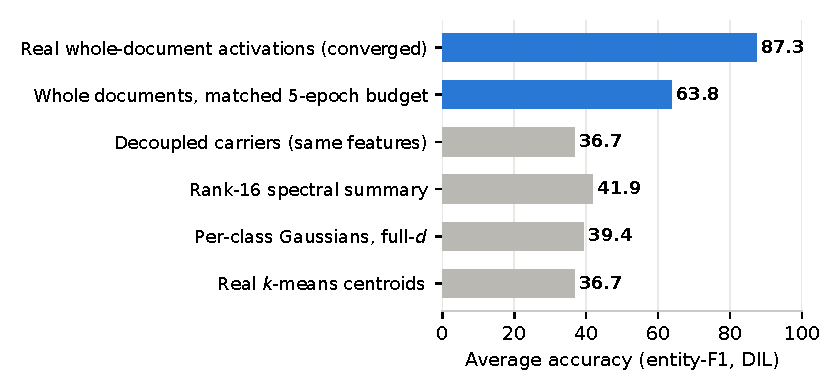
\includegraphics[width=0.8\textwidth]{paper/falsification_ladder.pdf}
  \caption[Memories that summarize against whole documents]{\textbf{Memories that
  summarize against whole documents} (DIL, one run each, earlier protocol). Only the
  replay of whole documents keeps the accuracy.}
  \label{fig:falsification-ladder}
\end{figure}

\end{appendices}

\end{document}
